% --------------------------------------------------------------------
% Modelo de Trabalho Acadêmico utilizando classe repUERJ para elaboração
% de teses, dissertação e trabalhos monográficos em geral.
%
% Este arquivo está editado na codificação de caracteres UTF-8.
%
% As referencia estão baseadas no modelo bibtex e citação em autor-data
%
% Este modelo foi adaptado pelo Prof. Irving Badolato
% Professor Assistente do Departamento de Engenharia Cartográfica
% Faculdade de Engenharia - FEN / Centro de Tecnologia e Ciências - CTC
% Universidade do Estado do Rio de Janeiro - UERJ
%
% A classe repUERJ.cls foi criada pelo Prof. Luís Fernando de Oliveira 
% do Instituto de Física, a partir do código original disponibilizado 
% pelo grupo CódigoLivre (coordenado por Gerald Weber).
% Foram feitas adequações para uso pelos alunos do curso de graduação 
% em Engenharia Cartográfica em acordo com as normas de elaboração de 
% teses e dissertações da UERJ.
%
% Os estilos repUERJformat.sty codificam os elementos pré-textuais e
% pós-textuais.
% O estilo repUERJpseudocode.sty codifica a elaboração de algoritmos
% utilizando um glossário desenvolvido pelo prof. Luís Fernando usado 
% em seu curso de Física Computacional.
%
% Este material está disponível também em:
% http://www.eng.uerj.br/~irvingbadolato/latex
%
% As normas da UERJ para elaboração de teses e dissertações pode ser
% obtidas no documento disponível no site:
% http://www.bdtd.uerj.br/roteiro_uerj_web.pdf
% --------------------------------------------------------------------
\documentclass[a4paper,12pt,oneside,onecolumn,final,fleqn]{formato/repUERJ}

% ********************************************************************
% Definição dos pacotes em uso neste documento
% Pacotes fundamentais 
\usepackage[utf8]{inputenc} % Determina a codificação utilizada
                            % (conversão automática dos acentos)
\usepackage[brazil]{babel}  % adequação para o português Brasil
\usepackage{makeidx}        % Cria o índice
\usepackage{hyperref}       % Controla a formação do índice
\usepackage{indentfirst}    % Endenta o primeiro paragrafo de
                            % cada seção.
\usepackage{graphicx}       % Inclusão de gráficos
\usepackage{subfig}
\usepackage{amsmath}        % pacote matemático
\usepackage{listings}       % Include the listings-package
\usepackage{microtype}
\usepackage{gensymb}
\usepackage{xcite}
\usepackage{float}
\usepackage{times}
\usepackage{tikz}
\usepackage{pdflscape}      % Recurso para páginas em paisagem. Útil nos anexos de grandes imagens.
\usetikzlibrary{fadings}

% Pacote auxiliar para as normas da UERJ
\usepackage[frame=no,algline=yes,font=default]{formato/repUERJformat}
\usepackage{formato/repUERJpseudocode}

% Pacotes de citações
\usepackage[alf]{abntex2cite}

% ********************************************************************


% ********************************************************************
% Informações de autoria e institucionais
%---------------------------------------------------------------------
% Imagens pretextuais (precisam estar no mesmo diretório deste arquivo .tex)
%---------------------------------------------------------------------
\logo{formato/logo_uerj_cinza.png}
\marcadagua{formato/marcadagua_uerj_cinza.png}{1}{160}{255}

%---------------------------------------------------------------------
% Informações da instituição
%---------------------------------------------------------------------
\instituicao{Universidade do Estado do Rio de Janeiro}
            {Centro de Tecnologia e Ciências} 
            {Faculdade de Engenharia} 
            {Departamento de Engenharia Cartográfica} 
             

%---------------------------------------------------------------------
% Informações da autoria do documento
%---------------------------------------------------------------------
\autor{Tatyana Vargas Queiroz} % Nome e sobrenomes do meio 
      {Vieira} % Último nome
      {T. V. Q.}      % Abreviação dos nomes iniciais

\titulo{Desenvolvimento de um Banco de Dados para o Laboratório de Fotogrametria e Sensoriamento Remoto}
\palavraschaves{Cartografia}
               {Banco de Dados Geoespaciais}
               {Fotogrametria}
               {Sensoriamento Remoto}
               {} % se não for usar a quarta palavra chave, deixar o campo vazio: {}

\title{Development of a Database for the Photogrammetry and Remote Sensing Laboratory}
\keywords{Cartography}
         {Geospatial Database}
         {Photogrametry}
         {Remote Sensing}

\orientador{Prof. Ph.D.} 
           {Jorge Luís}{Nunes e Silva Brito} 
           {Faculdade de Engenharia -- UERJ} 

%coorientador é opcional
\coorientador{Prof. Me.} 
             {Irving}{da Silva Badolato}
             {Faculdade de Engenharia -- UERJ} 

%---------------------------------------------------------------------
% Grau pretendido (Doutor, Mestre, Graduado, Bacharel, Licenciado, Engenheiro), % Curso (Engenharia Cartográfica, Engenharia Ambiental, Engenharia Elétrica) e 
% Gênero (Masculino, Feminino)
%---------------------------------------------------------------------
\grau{Engenheiro}  
\curso{Engenharia Cartográfica}
\genero{Feminino}

%---------------------------------------------------------------------
% Informações adicionais (local, data e paginas)
%---------------------------------------------------------------------
\local{Rio de Janeiro} 
\data{10}{12}{2019} % <= Atualize com a data da defesa

% ********************************************************************

% ********************************************************************
% Início do documento
\begin{document}
% ********************************************************************
% Configuração para iluminação de códigos
% ********************************************************************
% Configuração para destaque da linguagem de programação usada no trabalho
\lstset{language=SQL,
  basicstyle=\footnotesize\ttfamily,
  breaklines=true,
  frame=single,
  morekeywords={bigint, returns, double, precision, replace, function, is, language},
  deletekeywords={value,name},
  literate=
  {á}{{\'a}}1 {é}{{\'e}}1 {í}{{\'i}}1 {ó}{{\'o}}1 {ú}{{\'u}}1
  {Á}{{\'A}}1 {É}{{\'E}}1 {Í}{{\'I}}1 {Ó}{{\'O}}1 {Ú}{{\'U}}1
  {à}{{\`a}}1 {è}{{\`e}}1 {ì}{{\`i}}1 {ò}{{\`o}}1 {ù}{{\`u}}1
  {À}{{\`A}}1 {È}{{\'E}}1 {Ì}{{\`I}}1 {Ò}{{\`O}}1 {Ù}{{\`U}}1
  {ä}{{\"a}}1 {ë}{{\"e}}1 {ï}{{\"i}}1 {ö}{{\"o}}1 {ü}{{\"u}}1
  {Ä}{{\"A}}1 {Ë}{{\"E}}1 {Ï}{{\"I}}1 {Ö}{{\"O}}1 {Ü}{{\"U}}1
  {â}{{\^a}}1 {ê}{{\^e}}1 {î}{{\^i}}1 {ô}{{\^o}}1 {û}{{\^u}}1
  {Â}{{\^A}}1 {Ê}{{\^E}}1 {Î}{{\^I}}1 {Ô}{{\^O}}1 {Û}{{\^U}}1
  {Ã}{{\~A}}1 {ã}{{\~a}}1 {Õ}{{\~O}}1 {õ}{{\~o}}1
  {œ}{{\oe}}1 {Œ}{{\OE}}1 {æ}{{\ae}}1 {Æ}{{\AE}}1 {ß}{{\ss}}1
  {ű}{{\H{u}}}1 {Ű}{{\H{U}}}1 {ő}{{\H{o}}}1 {Ő}{{\H{O}}}1
  {ç}{{\c c}}1 {Ç}{{\c C}}1 {ø}{{\o}}1 {å}{{\r a}}1 {Å}{{\r A}}1
  {€}{{\euro}}1 {£}{{\pounds}}1 {«}{{\guillemotleft}}1
  {»}{{\guillemotright}}1 {ñ}{{\~n}}1 {Ñ}{{\~N}}1 {¿}{{?`}}1
}
% ********************************************************************

% ----------------------------------------------------------
% ELEMENTOS PRE-TEXTUAIS
\frontmatter
\capa
\folhaderosto

% ----------------------------------------------------------
% Inserir a ficha catalográfica
% ----------------------------------------------------------
% A biblioteca deverá providenciar a ficha catalográfica. Salve a ficha no formato PDF.
% Use o nome do arquivo PDF como argumento do comando. Exemplo: 
% Ficha catalográfica no arquivo 'ficha.pdf'
%\fichacatalografica{ficha.pdf}
% Enquanto não possuir a ficha catalográfica, use o comando sem argumentos...
\fichacatalografica{pretexto/ficha.pdf}


% ----------------------------------------------------------
% Folha de aprovação
% ----------------------------------------------------------
% membros da banca: máximo 6
%\begin{folhadeaprovacao}
  \assinatura{Prof. D.Sc. João Araújo Ribeiro}{Faculdade de Engenharia - UERJ}
  \assinatura{Prof.$^a$ Dra. Sonia Maria Lima Silva}{Faculdade de Engenharia - UERJ}
%  \assinatura{terceiro membro titular da banca}{instituição}
% suplente só é incluído se efetivamente substitui um titular
%  \assinatura{primeiro membro suplente da banca}{instituição}
%  \assinatura{segundo membro suplente da banca}{instituição}
%  \assinatura{terceiro membro suplente da banca}{instituição instituição instituição instituição }
\end{folhadeaprovacao}
\fichacatalografica{pretexto/aprov_tatyana.pdf}
% ----------------------------------------------------------
% Dedicatória
% ----------------------------------------------------------
\pretextualchapter{Dedicatória}

\vfill
À minha mãe, Senhora Maria Eny.

À minha família.

Aos meus amigos.

Por todo o suporte, paciência e ensinamento que me fizeram chegar até esse momento de realização deste trabalho.


% ----------------------------------------------------------
% Agradecimentos
% ----------------------------------------------------------
\pretextualchapter{Agradecimentos}

Agradeço à minha mãe, Senhora Maria Eny, por me ensinar que coragem é enfrentar seus medos para ir atrás de seus sonhos, à entender que nada na vida se conquista sem esforço, por me acompanhar em todos os passos de minha vida até este momento e acima de tudo por acreditar que eu seria capaz de chegar onde cheguei.

Agradeço aos meus orientadores, que acreditaram no meu potencial ao me confiar um projeto de tamanha complexidade, que sempre estiveram presentes nas inúmeras vezes em que precisei consultar-los me dando suporte mesmo em momentos em que não realizei que precisava de suporte.

Agradeço à minha família, que até mesmo com atos pequenos me ajudaram de forma gigantesca ao longo de todo este trabalho.

Agradeço aos meus amigos, que me emprestavam seus ouvidos em madrugadas à fora e nunca deixaram de me motivar, mesmo nos momentos onde a `Dona Murphy' mais me incomodou.

Agradeço aos Professores da Carto, por me emprestar seus conhecimentos em até mesmo horas aleatórias no meio do corredor da faculdade.



% ----------------------------------------------------------
% Epigrafe (opcional)
% ----------------------------------------------------------
\pretextualchapter{}

  \vfill\
  \begin{flushright}
    A felicidade não se resume na ausência de problemas, mas na sua capacidade de lidar com eles.

\textit{Albert Einstein}
  \end{flushright}

% ----------------------------------------------------------
% RESUMO
% ----------------------------------------------------------
\pretextualchapter{Resumo}

\fazreferencia

% Indicativo do trabalho:
% Entendimento do trabalho sem precisar ler o trabalho todo
% somente um parágrafo de 150 a 500 palavras segundo abnt,
% frases afirmativas curtas em voz ativa, 3 pessoa singular

% O que é (contexto)
Este trabalho tem como objetivo desenvolver um banco de dados que atenda ao acervo do Laboratório de Fotogrametria e Sensoriamento Remoto (LFSR) da Universidade do Estado do Rio de Janeiro (UERJ).
%relevância
Sua justificativa se dá pela carência na organização, armazenamento persistente em meio digital e acessibilidade aos dados brutos do acervo e também aos resultantes de projetos de mapeamento fotogramétrico realizados no LFSR da UERJ.
% Como? (Método utilizado)
A metodologia utilizada é composta por um levantamento de requisitos; uma modelagem UML segundo o paradigma de Orientação a Objetos (OO); a implementação de código-fonte; a realização da carga e testes de usabilidade. No caso particular de carga e visualização das imagens, foram utilizados scripts em python e o software QGIS.
% Resultados:
Os resultados incluem uma instância de banco de dados objeto-relacional implementada num servidor postgresql, com sua extensão espacial (postgis), para quatro conjuntos de projetos fotogramétricos do LFSR. Os testes realizados incluíram a elaboração de buscas para verificar a implementação e a validação quanto ao atendimento dos requisitos. Tais testes mostraram que o modelo pode ser adotado para diversos projetos simultâneos, permitindo sua comparação e o reaproveitamento de informações.
% Por quê? (Descreva o objetivo do trabalho):
Uma das conclusões do trabalho foi a de que o banco de dados proposto servirá para armazenar, em meio digital, os dados disponíveis que, atualmente, encontram-se em estado físico ou `\textit{hardcopy}', bem como para organizar dados digitais de projetos pré-existentes LFSR. Espera-se que este banco também possa vir a ser usado como ferramenta de aprendizagem para os alunos do curso de Engenharia Cartográfica, tanto nas matérias de Fotogrametria e Sensoriamento Remoto, quanto nas disciplinas relacionadas à Computação Aplicada à Cartografia.
% Conclui-se que:
Espera-se também que o modelo possa servir de base para novos projetos e, quando ampliado, para contemplar áreas não desenvolvidas até o momento por este laboratório, tal como uso de imagens orbitais ou a sua integração com a Infraestrutura Nacional de Dados Espaciais (INDE) ou com a restituição estereofotogramétrica realizada diretamente no padrão da Estrutura de Dados Geoespaciais Vetoriais (EDGV).
% Onde os resultados foram disponibilizados:
Os resultados deste trabalho estão disponíveis em \url{https://github.com/T4tyana/TCC}.
 
\imprimirchaves

% ----------------------------------------------------------
% Abstract
% ----------------------------------------------------------
\pretextualchapter{Abstract}

\doreference

%%%
This work aims to the development of a database for organizing the airborne imagery collection of the Photogrammetry and Remote Sensing Laboratory (LFSR) of the Rio de Janeiro State University (UERJ).
%%%
The proposed database will be used to the permanent storing in digital media of photogrammetric data, currently available only in physical or `hardcopy ' format. 
%%%
The modeling was developed using the UML, following the OO modeling paradigm; the implementation of the source code; the database uploading, and the usability tests. Python scripts and QGIS software were used for the visualization of in the particular case of photogrammetric imagery.
%%%
As a result of this work a relational-object database was generated and implemented with a postgresql/postgis software tool. Its initial loading was composed by four basic projects obtained through the LFSR. The tests for checking and validation of this database have shown that the model is effective and efficient. The tests also showed that the developed model could be used for many projects simultaneously, thus permitting comparisons between data sets, as well as reusing of stored information. 
%%%
One of the conclusions is that the proposed database will serve for its intended goals.
%%%
One expects that this database could be used as a learning tool for the subjects of photogrammetry and remote sensing, as well as for the computer aided cartography.
One expects that this model will serve as a base for new projects and when extended, for encompassing of new photogrammetric data, such as spaceborne imagery, and also for the integration with both the National Spatial Data Infrastructure (INDE) and the Vector Geospatial Data Structure (EDGV) brazilian data structures.
%%%
The results of this work are available at \url{https://github.com/T4tyana/TCC}.












\printkeys

% ----------------------------------------------------------
% Listas de ilustrações e tabelas
% ----------------------------------------------------------
\listadefiguras
\listadetabelas

% ----------------------------------------------------------
% Outras listas
% ----------------------------------------------------------
%\listadealgoritmos

% ----------------------------------------------------------
% Lista de abreviaturas e siglas
% ----------------------------------------------------------
\pretextualchapter{Lista de abreviaturas e siglas}

\abreviatura{API:        }   {\textit{Application Programming Interface}}
\abreviatura{DER:	     }   {Diagrama Entidade Relacionamento}
\abreviatura{EPSG:	     }   {\textit{European Petroleum Survey Group}}
\abreviatura{GML:	     }   {\textit{Geography Markup Language}}
\abreviatura{LFRS:}{Laboratório de Fotogrametria e Sensoriamento Remoto}
\abreviatura{CARTO:}{Departamento de Engenharia Cartográfica}
\abreviatura{UNESCO:}{Organização das Nações Unidas para a Educação, a Ciência e a Cultura}
\abreviatura{REA:}{Recurso Educacional Aberto}
\abreviatura{DSM:}{\textit{Digital Surface Model}}
\abreviatura{cp:}{centro de perspectiva}
\abreviatura{REM:}{Radiação Eletromagnética}
\abreviatura{NASA:}{\textit{National Aeronautics and Space Administration}}
\abreviatura{GIS:}{\textit{Geographic Information Systems}}
\abreviatura{SIG:}{Sistemas de Informações Geográficas}
\abreviatura{SGBD:}{Sistema Gerenciador de Banco de Dados}
\abreviatura{DBA:}{\textit{Database Administrator}}
\abreviatura{SQL:}{\textit{Structured Query Language}}
\abreviatura{SGBDOR:}{Sistema Gerenciador de Banco de Dados Objeto-Relacional}
\abreviatura{ISO:}{\textit{International Organization for Standardization}}
\abreviatura{ANSI:}{\textit{American National Standards Institute}}
\abreviatura{TDD:}{\textit{Test Driven Development}}
\abreviatura{RUP:}{\textit{Rational Unified Process}}
\abreviatura{UML:}{\textit{Unified Modeling Language}}
\abreviatura{CEMG:}{Comitê de Estruturação de Metadados Geoespaciais}
\abreviatura{CONCAR:}{Comissão Nacional de Cartografia}
\abreviatura{PK:}{\textit{Primary key}}
\abreviatura{FK:}{\textit{Foreign Key}}
\abreviatura{EPSG:}{\textit{European Petroleum Survey Group}}
\abreviatura{Gsd:}{\textit{Ground sample distance}}
\abreviatura{IPP:}{Instituto Municipal de Urbanismo Pereira Passos}
\abreviatura{SRS:}{\textit{Spacial Reference System}}
\abreviatura{WKT:}{\textit{Well-Known Text}}
\abreviatura{GDAL:}{\textit{Geospatial Data Abstraction Library }}
\abreviatura{OGC:}{\textit{Open Geospatial Consortium}}
\abreviatura{PNGB:}{Perfil de Metadados do Brasil}

% Adicionar outras abreviaturas aqui...
%% ----------------------------------------------------------
% Lista de simbolos
% ----------------------------------------------------------
\pretextualchapter{Lista de símbolos}
\simbolo{simbolo1}{significado e/ou valor}
\simbolo{simbolo2}{significado e/ou valor}
\simbolo{simbolo3}{significado e/ou valor}


% ----------------------------------------------------------
% Sumario
% ----------------------------------------------------------
\sumario


% ----------------------------------------------------------
% ELEMENTOS TEXTUAIS
% ----------------------------------------------------------
\mainmatter
%\include{capitulos/modelo}
\chapter*{introdução}

%NOTA: O texto que segue, com comentários (em latex) é importante exemplo baseado em trabalho de aluno anterior do Carto. Observe o modelo de texto em ch0.tex e edite-o para seu projeto final de curso adicionando sempre que possível perguntas relacionadas ao seu tema, como comentários, para orientar sua escrita e documentar o processo de elaboração de cada parágrafo. Tais comentários ajudam o aluno, a escrever, e podem ser complementadas no futuro com demais questões impostas pelo orientador ou pela banca. 

%O que são dados?
Todo trabalho, estudo ou desenvolvimento tecnológico possui objetivos, resultados e utiliza um método. Uma das partes mais importantes de um esforço de desenvolvimento científico-tecnológico são os dados. Na realidade os dados estão presentes: no início, sobre os quais a hipótese científica será testada; no momento em que esses dados são analisados e trabalhados; e no fim, onde os dados finais obtidos são chamados de resultados. Assim, pode-se dizer que `dado' é todo e qualquer insumo utilizado na realização de um trabalho. 
%Qual a importância da organização de dados?
Por outro lado, dado por si só é um fato isolado que pode ou não ser relevante para um projeto. Sua organização permite que o pesquisador entenda qual é sua viabilidade e a forma que melhor se adéqua ao desenvolvimento do trabalho. 

A sociedade atual vive o que se chama de `Era Digital', onde programas de computador são capazes de processar inimagináveis volumes de dados, de forma rápida e eficiente e, preservando esses dados em caráter permanente. O meio digital pode ser reconhecido como uma excelente forma de armazenamento de dados.

% Qual é o objeto de estudo deste trabalho?
Este trabalho tem por objetivo geral o desenvolvimento de um banco de dados para a organização do acervo técnico do Laboratório de Fotogrametria e Sensoriamento Remoto (LFSR) do Departamento de Engenharia Cartográfica da Universidade Estadual do Rio de Janeiro - UERJ. 

Como objetivos específicos, listam-se os seguintes:
\begin{itemize}
\item Revisão da literatura técnica sobre bancos de dados, com ênfase em bancos de dados geoespaciais;
\item Seleção do modelo conceitual a ser utilizado;
\item Levantamento dos requisitos para o banco a ser desenvolvido;
\item Modelagem do banco de dados, segundo a abordagem orientada a objetos;
\item Implementação do banco segundo a metodologia ágil;
\item Armazenamento do banco de dados;
\item Testes do banco de dados, por intermédio do desenvolvimento de consultas típicas, baseado no levantamento de requisitos.
\end{itemize}

% Qual a importância do laboratório no departamento de cartografia?
O LFSR é essencial para o processo ensino-aprendizagem dos alunos do curso de graduação de Engenharia Cartográfica. Além disso é importante para a disseminação do conhecimento relevante à disciplina de Fotogrametria Digital, para alunos externos e pesquisadores da área. O acervo do LFSR possui inúmeros dados, como fotogramas que se apresentam em formato analógico (em papel fotográfico), o que vem dificultando a organização e utilização dos mesmos. Grande parte do acervo do laboratório pode ser aproveitado para futuros projetos dos alunos do curso, porém o acervo fotográfico do Laboratório, em formato de papel, tem implicado na perda desses dados por efeito do tempo e das condições de armazenamento do material.

% Como isso se encaixa no curso de Cartografia?
A Engenharia Cartográfica, por sua vez, tem como objetivo geral o mapeamento de uma área geográfica de interesse. Uma das formas de realização dessa tarefa é através da utilização de técnicas de mapeamento Fotogramétrico. Com o atual estágio do desenvolvimento científico-tecnológico, no contexto da Engenharia Cartográfica, os produtos do mapeamento, de uma maneira geral, são realizados por intermédio de computadores digitais, dando origem ao conceito de dados e informações geoespaciais. Essas informações necessitam ser organizadas e armazenadas, em estruturas de dados vetoriais e matriciais, requerendo, na maior parte das vezes, a análise, o projeto e a implementação de um banco de dados geoespaciais. Este fato demonstra, com clareza, a importância do conceito e a aplicabilidade de um banco de dados na área de Engenharia Cartográfica.

%Organização do dados - qual é a necessidade de um banco?
A solução idealizada neste trabalho, para organização dos dados em meio digital, requer a análise de requisitos, projeto e implementação de um banco de dados modelado a partir das necessidades do laboratório. Além disso fez-se necessário entender o potencial do uso deste banco como uma nova ferramenta, não só de armazenamento, mas também de aprendizado para as disciplinas que fazem uso desse laboratório. 
O projeto piloto do banco engloba grande parte do processo aerofotogramétrico, e deixa, em aberto, possibilidades para futuras expansões que venham a incluir processos de dados de sensoriamento remoto além dos obtidos pela fotogrametria aérea tradicional.

%Dados fotogramétricos:
O banco de dados proposto, como dito previamente, foca na fotogrametria, cujo objetivo principal corresponde a reconstrução de um espaço 3D, a partir de imagens 2D, de forma a representar, georreferenciar e medir o objeto imageado da forma mais fiel possível. Um banco de dados fotogramétrico, por sua vez, armazena todas as informações pertinentes à aquisição das imagens e seu subsequente processamento, de forma que o projeto fotogramétrico seja preservado e reutilizado. Essa linha de pensamento será desenvolvida ao longo do trabalho. 

% Qual é a organização deste trabalho? 
Este trabalho é estruturado em três capítulos, além da Introdução, Conclusão, Referências, Apêndices e Anexos. O primeiro consiste na fundamentação teórica que dê ao leitor o embasamento necessário para que o mesmo seja capaz de entender como este trabalho foi realizado. O segundo capítulo trata da metodologia, e apresenta como o modelo proposto foi desenvolvido, desde um primeiro momento, onde ocorre o levantamento de requisitos, até a geração do código base, usado para a implementação do banco de dados piloto. O terceiro capítulo, por sua vez, apresenta os resultados gerados e testes do projeto piloto, bem como a discussão proveniente dos mesmos. Por fim, uma breve conclusão e referências bibliográficas são apresentadas.
%=====================================================================
\chapter{Fundamentação teórica}\label{chp}
%========================================================

Como este trabalho propõem a elaboração de um modelo de banco de dados para o LFSR da UERJ, o Capítulo \ref{chp} apresenta conceitos julgados relevantes à metodologia desenvolvida na criação desse projeto piloto. %exemplificar? 



\section{Laboratório de Fotogrametria e Sensoriamento Remoto - LFSR}

O laboratório de Fotogrametria e Sensoriamento Remoto - LFSR faz parte do Departamento de Engenharia Cartográfica - CARTO da Universidade do Estado do Rio de Janeiro - UERJ. Suas instalações são utilizadas para aulas e trabalhos práticos nas disciplinas de Fotogrametria Básica, Fotogrametria Analógica e Analítica, e Aerotriangulação. Uma equipe técnica composta por Professores da UERJ e alunos voluntários e estagiários é responsável pela organização e manutenção de seu espaço físico e seu acervo. O LFSR conta também com o Projeto E-Foto desde Agosto de 2004 em suas instalações, usado como ferramenta auxiliar no aprendizado dos alunos da área.  

\subsection{Instalações do Laboratório de Fotogrametria e Sensoriamento Remoto}

O LFSR se encontra no quarto andar, sala 4044-F, da UERJ. Possui em suas instalações os seguintes equipamentos de fotogrametria, em sua maior parte analógicos: 

\begin{itemize}
    \item Um Aviógrafo Kern PG2 para estéreo compilação fotogramétrica;
    \item Um Aerotriagulador Analógico do tipo Estereoplanígrafo C3;
    \item Quinze Estereoscópios de espelhos;
    \item Centenas de fotogramas em papel e alguns exemplares em diapositivos;
    \item Um Digitalizador Matricial (Scanner) A3Microtek ScanMaker 9800XL;
\end{itemize}

O laboratório também possui computadores (6 desktops e 3 laptops) e algumas poucas licenças de software comercial, priorizando o desenvolvimento e/ou instalação de software livre para a Fotogrametria em seus equipamentos. Seu acervo de dados é composto em sua grande maioria de fotogramas impressos em papel que caracterizam-se de aerolevantamentos passados doados ao Departamento de Cartografia. A figura \ref{lab} representa um demonstrativo dos materiais disponíveis nas instalações do laboratório.

\begin{figure}[!ht]{10cm}
  \caption{Apresentação das instalações e equipamentos do LFSR} \label{lab}
  \centering
  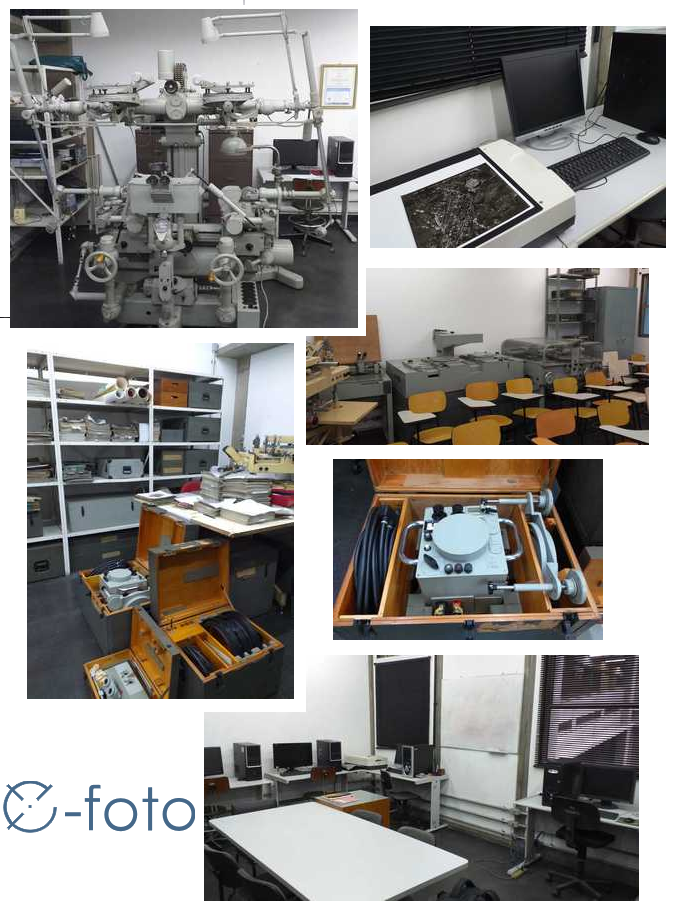
\includegraphics[width=1\textwidth]{figuras/lab.png}
  %\legend{}
  \source{A autora, 2019}
\end{figure}

A ideia da preservação deste acervo, por intermédio da digitalização matricial foi um das motivações para o desenvolvimento deste trabalho. Outro fator motivador foi a necessidade de organizar o acervo, visando não somente ao armazenamento do mesmo mas, principalmente, à sua divulgação e potencial de uso pelos estudantes e professores do Departamento de Engenharia Cartográfica e demais instituições de ensino.

\subsection{Projetos Existentes no Laboratório de Fotogrametria e Sensoriamento Remoto}\label{efoto}

Todo laboratório com fim educacional em geral fornece a infraestrutura necessária para o desenvolvimento de um ou mais projetos que o habilita a exercer sua função acadêmica. O LFSR por sua vez trabalha com o projeto de desenvolvimento do software livre e-foto\footnote{Adota-se a grafia \textit{e-foto} para referir-se ao software e \textit{E-Foto} para referir-se ao seu projeto de desenvolvimento}.

``O projeto E-Foto prevê a implementação de uma solução de uma estação fotogramétrica digital para fins educacionais, de forma livre, habilitando o acesso a tal informação a quaisquer pessoas que o queiram.'' \cite[p. 9]{coelho2007fotogrametria}.

Corroborando com \citeonline{devauxteste}, um `software livre' deve permitir que o usuário: consiga utilizar do programa para quaisquer fins, tenha permissão de redistribuir do programa com a intenção auxiliar outros usuários, a liberdade de aperfeiçoar o software e difundir esses aperfeiçoamentos, e por fim que a plataforma seja de código aberto. Como o projeto E-Foto se enquadra nessas características, além de ser um software com fim educacional, o mesmo atende ``a proposta definida pela Organização das Nações Unidas para a Educação, a Ciência e a Cultura (UNESCO), como um Recurso Educacional Aberto (REA)'' \cite[p.1032]{tramontina69analise}.

De acordo com \citeonline{aguiar2010:desc} o projeto E-Foto conta com vários documentos e dados como tutoriais, trabalhos acadêmicos relacionados ao projeto, o próprio software e etc, em um site próprio com visitas de todo o mundo o que, segundo os autores caracteriza a importância do projeto E-foto como iniciativa no meio acadêmico para a área de Fotogrametria. 

Assim sendo, alunos e pesquisadores da área que usufruem das instalações do LFSR são contemplados com uma plataforma capaz de auxiliar na implementação e ensinamento do processo fotogramétrico. Os resultados de tal uso persistem atualmente sob a forma de arquivos digitais (em formato próprio do software) dos projetos fotogramétricos realizados neste software. Então, a modelagem do banco de dados discutida no capítulo \ref{met} deverá considerar como parte dos requisitos o suporte às informações dos dados dos trabalhos realizados dentro do LFSR. 

Destaca-se também a relevância dos dados de exemplo adotados nos tutoriais publicados no contexto do projeto E-Foto. Por sua importância os mesmos foram selecionados como parte dos dados e documentos que foram usados para a carga inicial e testes do banco de dados desenvolvido nesse trabalho, como será apresentado na seção \ref{carga}.

O processo fotogramétrico possui diversas atividades que podem variar de acordo com o software, porém existem algumas atividades comuns que devem ser destacadas, sendo a maioria identificada facilmente no fluxograma de trabalho da plataforma E-foto, como visto na figura \ref{flux}.

\begin{figure}[!ht]{10cm}
  \caption{Fluxograma de trabalho da plataforma E-foto} \label{flux}
  \centering
  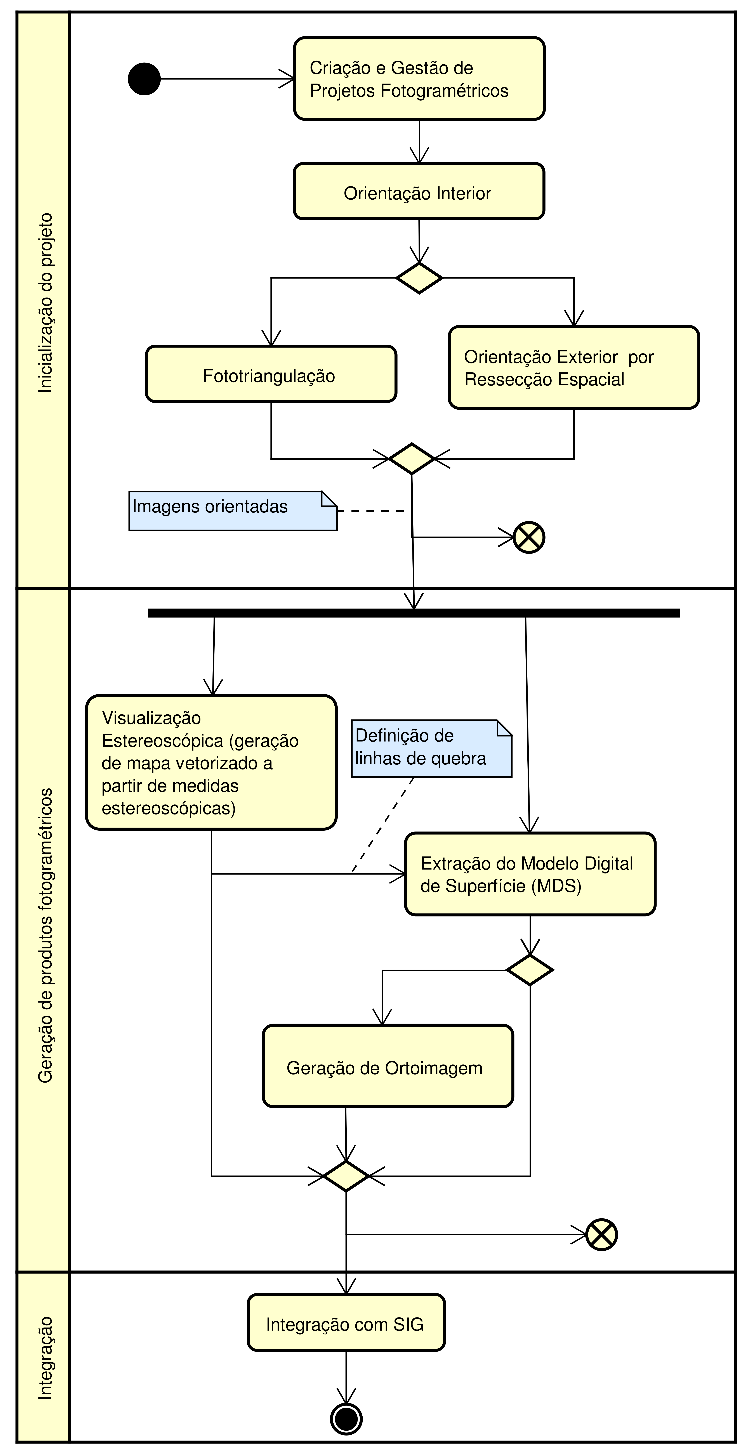
\includegraphics[width=1.2\textwidth, height=1.75\hsize]{figuras/efoto_flux.png}
  %\legend{Texto da legenda quando necessário.}
  \source{\cite{efotoWorkflow}}
\end{figure}

Essas atividades estão distribuídas em 3 fases do projeto. As fases transmitem a compreensão do grau de desenvolvimento do projeto fotogramétrico. Tais fases e atividades são descritas a seguir:

\begin{enumerate}
    \item \textbf{Inicialização do Projeto:} Antes que qualquer produto da fotogrametria possa ser gerado e divulgado para demais processos de produção cartográfica é necessária a realização da aquisição, do cadastro e da orientação (ajustamento) dos dados. Tais atividades são tratadas como fase inicial, pois não produzem produtos finais para processos externos à fotogrametria. As atividades nesta fase são:
    \begin{itemize}
        \item \textbf{Criação e Gerenciamento do Projeto Fotogramétrico:} Nesta atividade do processo o responsável técnico pelo projeto registra os metadados como os obtidos a partir do certificado de calibração e planejamento de voo, que são indispensáveis para os cálculos. No momento inicial de um projeto fotogramétrico ocorrem os levantamentos aéreo e topográfico da região de interesse, resultando na aquisição de dados como as imagens e os pontos de apoio de campo que serão usados no processamento. Esta atividade incluí também o cadastro dos dados adquiridos como resultado dos levantamentos realizados.
        \item \textbf{Orientação Interior:} Nesta atividade do processo as imagens estão sem a referência métrica, tendo suas coordenadas relativas aos \textit{pixels}, isto é, em `linhas' e `colunas'. Logo deve ser feita a reconstrução do feixe perspectivo, um processo que precisa de informações como as coordenada do centro de perspectiva (CP) da câmara e a distância focal. Como resultado são ajustados coeficientes para um modelo paramétrico que relacionam o sistema matricial da imagem com o sistema métrico do sensor por intermédio, por exemplo, da transformação afim\footnote{Apontamentos de aula da disciplina Fotogrametria Analógica e Analítica ministrada pelo Professor Jorge Luís N. e S. Brito}.
        \item \textbf{Orientação Exterior:} A orientação exterior consiste na determinação da posição tridimensional do centro de perspectiva da câmara, em relação ao referencial de coordenadas do terreno, e dos seus respectivos ângulos de atitude, no momento da tomada da fotografia. O cálculo consiste na determinação de seis parâmetros: as coordenadas no espaço-objeto do centro de perspectiva (X0,Y0,Z0) e os ângulos de atitude do sensor ($\phi$,$\omega$,$\kappa$). É importante mencionar que o cálculo dos parâmetros da orientação exterior pode ser realizado para cada imagem isoladamente (atividade de ressecção espacial) ou para o conjunto de imagens que compõem um bloco fotogramétrico, situação na qual o processo adota a atividade de fototriangulação (também conhecida como aerotriangulação).
    \end{itemize}
    \item \textbf{Geração de Produtos:}  Nesta fase são gerados o produtos fotogramétricos propriamente, dentre os quais o projeto E-Foto inclui:
    \begin{itemize}
        \item \textbf{Visualização Estereoscópica:} Permite a observação de modelos estereoscópicos e a restituição fotogramétrica, isto é, a vetorização de superfícies pela obtenção de seus vértices em três dimensões. São produzidas nesta atividade feições vetoriais como pontos, linhas e polígonos.
        \item \textbf{Extração de Modelo Digital de Superfície:} Permite a modelagem da superfície observadas nas imagens do projeto fotogramétrico pela extração automatizada de pontos tridimensionais sobre a superfície. Métodos de interpolação para publicação de modelos regulares são inclusos nesta atividade.
        \item \textbf{Geração de Ortoimagem:} Uma ortoimagem é, por definição, uma imagem que passou pelo processo de ortoretificação e teve os deslocamentos devido ao relevo, removidos nesse processo. Esta atividade se concentra na ortoretificação para imagens isoladas ou blocos. No último caso o produto é chamado de ortomosaico.
    \end{itemize}
    \item \textbf{Integração:} A fase de integração admite que os produtos fotogramétricos sejam disponibilizados nos formatos próprios para uso em demais processos de produção cartográfica. Embora as atividades desta fase possam ser diferenciadas de acordo com o produto fotogramétrico e processo de produção cartográfica, o diagrama simplifica esta fase em uma atividade.
\end{enumerate}

Devido a extensão do fluxo de trabalho, conforme será discutido no capítulo \ref{met}, o escopo da modelagem deverá ser delimitado nas atividades da fase de inicialização do processo fotogramétrico.



\section{Sensoriamento Remoto e Fotogrametria} \label{sensofot}
Sensoriamento Remoto é mais comumente conhecido como uma ciência e técnica que tem por objetivo a captação de informações sobre um objeto, onde não existe contato físico entre o sensor e o objeto de interesse.  Enquanto essa definição não é errada, esta por si só é demasiadamente ampla, o que leva à uma definição mais científica: 

``Sensoriamento Remoto é uma ciência que visa o desenvolvimento da obtenção de imagens da superfície terrestre por meio da detecção e
medição quantitativa das respostas das interações da radiação eletromagnética com os
materiais terrestres.'' \cite[p.3]{meneses2012introduccao}

\subsection{Espectro Eletromagnético}
Os dados obtidos por um processo de sensoriamento remoto dependem da energia com que trabalha o sensor, essa energia é a radiação eletromagnética - REM (ou simplesmente energia eletromagnética), que se propaga no vácuo em forma de senoides, com variações de frequência e comprimento de onda. A figura \ref{wave} ilustra a propagação de uma onda eletromagnética.

\begin{figure}[!ht]{12cm}
  \caption{Representação da propagação de uma onda eletromagnética.} \label{wave}
  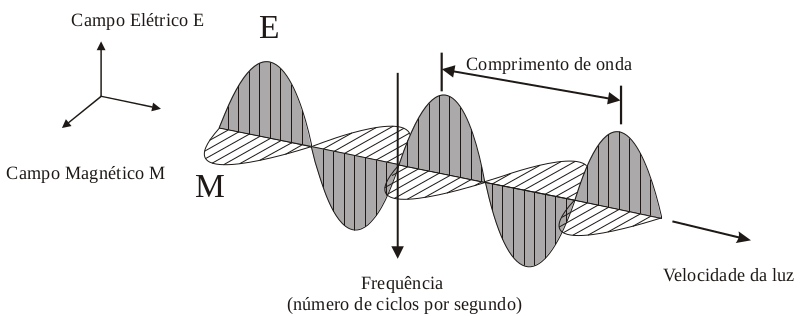
\includegraphics[width=1.1\hsize]{figuras/wave.png}
  %\legend{Texto da legenda quando necessário.}
  \source{\cite{florenzano2007iniciaccao}}
\end{figure}

``Denomina-se espectro eletromagnético as regiões espectrais da REM conhecidas pelo
homem.'' \cite[p.18]{meneses2012introduccao}
De acordo com \citeonline[p.21-24]{moreira2007fundamentos} o espectro eletromagnético possui uma grande variação em seus comprimentos de onda, onde seu comprimento é inversamente proporcional à sua frequência. Isso implica em que nas regiões do espectro onde as ondas são mais curtas, e associadas aos raios cósmicos, a frequência é muito maior do que nas regiões de ondas mais longas, região onde se encontram as ondas longas de rádio frequência.
Essas regiões são apresentadas na figura \ref{espectro}.

\begin{figure}[!ht]{12cm}
  \caption{Ilustração do Espectro Eletromagnético.} \label{espectro}
  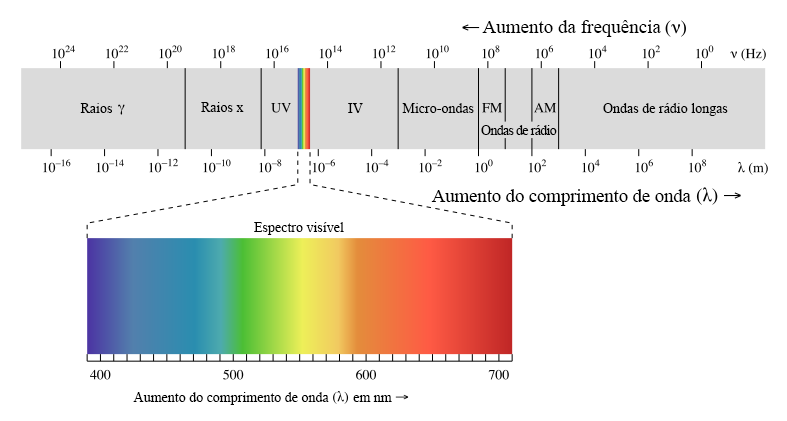
\includegraphics[width=1.1\hsize]{figuras/espectro.png}
  %\legend{Texto da legenda quando necessário.}
  \source{\cite{admirdoresdafisica}}
\end{figure}

Enquanto o olho humano só é capaz de enxergar um intervalo do espectro magnético conhecido como 'luz visível', um sensor remoto é capaz de captar informações espectrais de outros comprimentos de onda de fora desse intervalo. 
\begin{citacao}
    
As imagens [...] devem ser vistas como uma forma de documentos que representam, em escala e sobre um plano 2D, os acidentes e as feições naturais e artificiais da superfície terrestre, a partir da medição de um processo físico da radiação eletromagnética.\cite[p.77]{meneses2012introduccao}
\end{citacao}
Durante anos a fotogrametria foi restrita a imagens fotográficas, somente possíveis pela captação e registro da parte visível do espectro eletromagnético, explicitado na figura \ref{espectro}, porém com os avanços tecnológicos os sensores atuais são capazes registrar informações além desse intervalo, abrindo inúmeras possibilidades para a fotogrametria.  

\subsection{Sensores e Captação de Imagens}\label{sensor_img}
``Os sensores remotos são equipamentos que captam e registram a energia refletida ou emitida pelos elementos da superfície terrestre'' \cite{florenzano2007iniciaccao}.
De acordo com \citeonline[p.9]{lillesand2015remote} a energia de radiação eletromagnética captada por esses sensores deve passar pela atmosfera terrestre.
Contudo, ``a atmosfera interfere na intensidade do fluxo radiante, na distribuição espectral e na direção dos raios incidentes, tanto na sua trajetória
descendente entre o Sol e a Terra como na trajetória ascendente da radiação refletida e
emitida da superfície terrestre para o sensor'' \cite[p.24]{meneses2012introduccao}.

Conforme \citeonline[p.9]{lillesand2015remote}, a energia utilizada pelo sensor remoto ao passar pela atmosfera sofre em seu caminho dois efeitos de distorção: \textit{espalhamento} e \textit{absorção}.

Espalhamento pode ser definido como a dispersão (ou difusão) da radiação eletromagnética por moléculas, ou partículas maiores, presentes na atmosfera. Quando o espalhamento é resultante da presença de moléculas muito menores do que a radiação tem-se o espalhamento \textit{Rayleigh}. Este, resulta normalmente no efeito `nebuloso' na imagem. Quando a partícula possui um tamanho de diâmetro similar ao comprimento da onda o espalhamento resultante é chamado de \textit{Mie}. Esse tipo de espalhamento é geralmente causado por poeira e vapor d'água. Por fim, quando essas partículas são muito maiores do que o comprimento de onda eletromagnético, denomina-se o espalhamento resultante de \textit{Não-Seletivo}. Este é considerado como o pior espalhamento para sensoriamento remoto, pois afeta tamanhos aleatórios de comprimentos de onda de radiação. Um exemplo simples de efeito na imagem é a presença de nuvens na mesma. O índice da presença de nuvens em uma imagem afeta a usabilidade desta em um projeto fotogramétrico e deve ser levada em consideração em momentos como na montagem do bloco de imagens a ser usado num projeto.

Absorção, ao contrário do espalhamento, resulta na perda da radiação. Devido à presença de gases na atmosfera que interagem diretamente com o espectro eletromagnético, a energia é `bloqueada' no caminho entre a fonte de energia e o alvo, ou no retorno, entre o alvo e o sensor remoto. Esta ocorrência gera as chamadas `janelas atmosféricas', que nada mais são do que os intervalos de comprimento de onda não-absorvidos na atmosfera e, portanto, captados pelo sensor.
%VERIFICAR COM NUNES SE ESTE PARÁGRAFO PRECISA SER MODIFICADO OU NÃO!!!!
Corroborando com \citeonline[p.12]{lillesand2015remote},  um sensor não deve ser escolhido arbitrariamente; ao escolhê-lo deve-se levar em consideração os seguintes aspectos:
\begin{itemize}
\item a sensibilidade do sensor;
\item as janelas atmosféricas existentes dentro do comprimento de onda em que se planeja trabalhar;
\item fonte, magnitude e composição espectral da energia de radiação a ser utilizada.
\end{itemize}

Existe um amplo leque de variedade de modelos e fabricantes de sensores remotos. Tendo em vista os efeitos discutidos nos parágrafos anteriores, trata-se agora a da classificação dos sensores.

Segundo \citeonline[p.98]{fitz2008cartografia}, sensores podem ser classificados de acordo com a origem da fonte de energia em  \textit{ativos} e \textit{passivos}.

Sensores ativos são aqueles que possuem fonte de energia interna (ou acoplada ao sensor). Isso significa que a energia necessária para captar a radiação refletida pelo alvo deve ser emitida pelo próprio sensor. O Radar é um bom exemplo desse tipo de sensor, fazendo a captação de dados por meio de ondas de rádio. A figura \ref{sr_ativo} ilustra de forma simplificada um sensor ativo.

\begin{figure}[!ht]{10cm}
  \caption{Ilustração de um sensor ativo} \label{sr_ativo}
  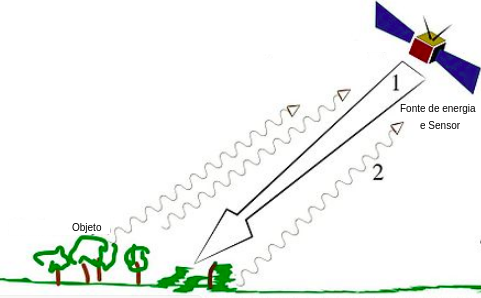
\includegraphics[width=1\hsize]{figuras/sensor_ativo.png}
  \legend{1. A energia é emitida de uma fonte artificial em direção à superfície; 2. A energia é refletida retorna para registro pelo sensor.}
  \source{Adaptação de \cite{sensorfig}}
\end{figure}

Sensores passivos, no entanto, dependem de uma fonte de energia externa e independente do sensor. O Sol é a fonte de energia externa com que trabalha a maioria dos sensores passivos. Neste caso a imagem, gerada precisa ser obtida necessariamente durante o dia. A figura \ref{sr_passivo} ilustra de forma simplificada um sensor passivo.

\begin{figure}[!ht]{10cm}
  \caption{Ilustração de um sensor passivo} \label{sr_passivo}
  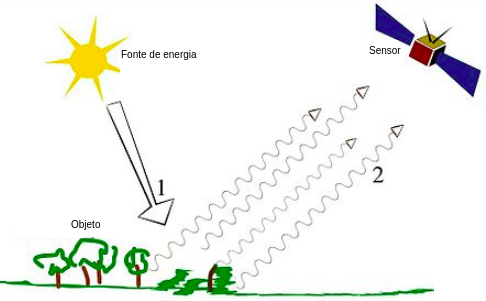
\includegraphics[width=1\hsize]{figuras/sensor_passivo.png}
  \legend{1. A energia é emitida de uma fonte natural e atinge a superfície; 2. A energia é refletida e retorna para registro pelo sensor.}
  \source{Adaptação de \cite{sensorfig}}
\end{figure}

Existem casos, como as câmeras fotográficas digitais, onde o sensor se enquadra em ambas as classificações. Se o `flash' da câmera estiver ativado, a fotografia gerada é proveniente de uma fonte interna, o que caracteriza o sensor como ativo. Porém, se o `flash' estiver apagado, a fotografia vai depender de uma fonte de energia externa, o que define, neste momento, a câmera como um sensor passivo.

De acordo com \citeonline[p.98]{fitz2018geoprocessamento}, outra forma de classificar o sensor é por seu produto. Estes sensores são conhecidos como \textit{imageadores} ou, \textit{não imageadores}. Sensores imageadores, como o próprio nome indica, traduz os dados em formato de imagens. Sensores não imageadores geram, a partir da informações coletadas, dados em formato de tabelas, gráficos e etc. Os dados de sensores não imageadores, geralmente chamados de spectroradiômetros, destinam-se a construir bibliotecas de assinaturas espectrais, que fogem ao escopo deste projeto. Por isso lida-se neste trabalho somente com o sensor imageador.

%falar sobre sensores, como eles funcionam(adicionar ilustração), a diferença entre orbital, comentando brevemente na diferença entre as geometrias de aquisição de imagens, e aéreo e enfatizar a importância do sensoriamento aéreo para o trabalho.
\subsection{Níveis de Aquisição de Imagens}
%nao tenho o texto da florenzano!!!! descobrir a pag!
Segundo \citeonline{florenzano2007iniciaccao} um sensor pode se encontrar em diferentes plataformas sejam elas, terrestres, aéreas ou orbitais.
\citeonline[p.3-4]{meneses2012introduccao} afirma que as fotografias são uma classe de sensores remotos. Isso corrobora a afirmação de que a Fotogrametria é uma forma de Sensoriamento Remoto. Assim sendo, ``convencionou-se usar a classificação de \textit{fotogrametria terrestre}, \textit{fotogrametria aérea} (ou aerofotogrametria) e \textit{fotogrametria orbital} para, grosso modo, expressar esses diferentes modos de posicionar o sensor.'' \cite[p. 18]{coelho2007fotogrametria}

A figura \ref{niveis_sr} ilustra os níveis de plataformas aos quais um sensor pode estar acoplado, o que por sua vez influenciam a distância entre um sensor e o objeto, e o tamanho da área que esse sensor consegue analisar. 

\begin{figure}[!ht]{10cm}
  \caption{Níveis de Plataformas de Coletas de Dados de Sensores.} \label{niveis_sr}
  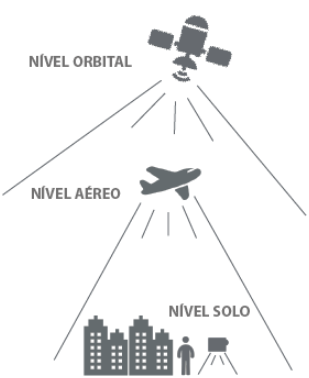
\includegraphics[width=0.5\hsize]{figuras/niveis_sr.png}
  %\legend{Texto da legenda quando necessário.}
  \source{\cite{sensoriamentoremotoweb}}
\end{figure}

Seguindo essa linha de pensamento e utilizando da classificação dada por \citeauthoronline{coelho2007fotogrametria} (\citeyear{coelho2007fotogrametria}, p.18), pode-se dizer que:
\begin{itemize}
    \item \textbf{Fotogrametria Orbital:} se refere a aquisição de imagens que ocorre em nível orbital onde o sensor está acoplado à um satélite. Um satélite por sua vez permanece em órbita durante seu tempo de vida útil transmitindo seus dados a um receptor que se encontra na Terra. Isso permite uma aquisição de imagens abundante onde, dependendo das especificações de seu sensor, podem ter altíssimas precisões muitas vezes necessárias em trabalhos cartográficos. Segundo \citeonline[p. 1]{aquiar2007google}, atualmente imagens de satélites são distribuídos pela internet por plataformas como Google Earth, Microsoft Visual Earth e NASA World Wind. 
    \item \textbf{Fotogrametria Aérea:} também chamada de Aerofotogrametria, acontece quando o sensor se encontra em plataformas de nível aéreo, como aviões e drones. Um exemplo de dados registrados nesse nível são as fotografias aéreas capturadas por câmeras fotográficas métricas. Este assunto será mais explorado posteriormente no item \ref{foto_trad}.
    \item \textbf{Fotogrametria Terrestre:} ou Curta-Distância, se caracteriza essencialmente pelos seus alvos de interesse e a câmara estarem geralmente fixos. A câmara possui seu eixo ótico horizontalizado, o que gera uma imagem horizontal. Essa fotogrametria ocorre no solo, ou a poucos metros acima deste, e investiga objetos geralmente com a intenção de analisar os componentes do mesmo para serviços especializados como a Topografia, a Arquitetura, a Engenharia Civil e etc. Nesses casos a finalidade pode variar de controle de deformação ou desgaste do objeto à restauração do patrimônio histórico de determinada edificação ou o próprio mapeamento topográfico de regiões de difícil acesso.  
\end{itemize}
% falar dos níveis, orbital etc.
Contudo, deve-se ressaltar que o Sensoriamento Remoto, independentemente do nível da plataforma de aquisição em que ocorre, se difere das Fotogrametrias Orbital, Aérea e Terrestre por englobar também sensores não-imageadores (explicados no item \ref{sensor_img}). Ou seja, a fotogrametria tem como foco extração da métrica 3D a partir das imagens 2D. Por outro lado o sensoriamento remoto pode também ter como foco determinar o significado de objetos imageados por interpretação de imagens. 

\subsection{Fotogrametria Aérea Tradicional}\label{foto_trad}
Segundo \cite[p. 16]{coelho2007fotogrametria}, a fotogrametria pode ser definida como ciência e tecnologia capaz reconstruir o espaço tridimensional, ou parte do mesmo (espaço-objeto), a partir das imagens 2D, oriundas da gravação de padrões de ondas eletromagnéticas (espaço-imagem), sem ter nenhum contato físico direto entre sensor e alvo de interesse.

Na Fotogrametria Aérea Tradicional para autores como \citeonline{projeto1999dalmolin}, \citeonline{coelho2007fotogrametria}, entende-se por plataforma um avião ou uma aeronave à qual o sensor está alocado.

Nos dias atuais, os sensores podem ser analógicos ou digitais. O projeto piloto contempla sensores analógicos que obtenham imagens quadro à quadro, em seus certificados de calibração deve estar registrado as informações relativas às marcas fiduciais. Isto se justifica pelo grande número de imagens deste formato existentes no acervo e como será percebido no capítulo \ref{met} o modelo atende a ambos os tipos de sensor, sendo apenas restrito até o momento aos sensores de quadro. Outros tipos de sensores incluem varredores, muito comuns nos satélites.

%FAZER MARCAÇÃO DA PAGINA!!!!
De acordo com \citeonline{wolf2014elements} a Fotogrametria Aérea pode ser subdividida em duas: \textit{Vertical} ou \textit{Oblíqua}. Na vertical o sensor tem seu eixo óptico alinhado verticalmente ao terreno, resultando em uma tomada de foto onde a projeção da imagem produzida fica em paralelo ao plano da região de interesse. A aeronave sofre porém, ao sobrevoar o terreno, leves alterações em seu curso que acarreta numa variação de angulação pequena e não intencional da foto em relação ao plano do terreno gerando assim fotos levemente inclinadas em ângulos geralmente num intervalo de 1$^{\circ}$ a 3$^{\circ}$. Estes são os ângulos de Euler, ou ângulos de atitude, comentados no capítulo \ref{met}. A Oblíqua por sua vez possui uma inclinação intencional onde a mesma pode ser alta a ponto de permitir ser visto a linha do horizonte na fotografia, como ilustrado na figura \ref{obliqua}.

\begin{figure}[!ht]{10cm}
  \caption{Ilustração da angulação e efeito de distorção em imagens geradas por Fotogrametria Aérea Oblíqua} \label{obliqua}
  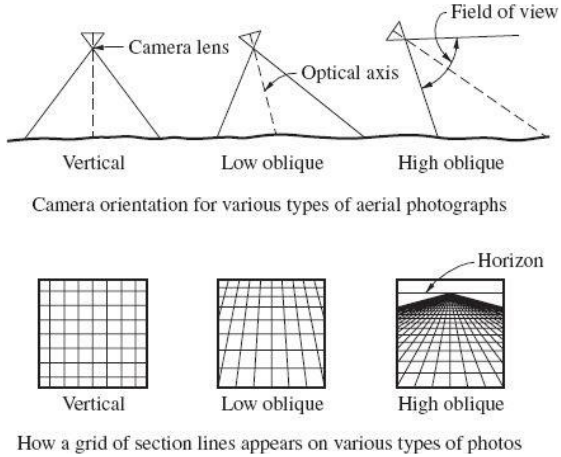
\includegraphics[width=0.75\hsize]{figuras/obliqua.jpg}
  %\legend{Texto da legenda quando necessário.}
  \source{\cite{wolf2014elements}}
\end{figure}

As Fotos geradas pela Fotogrametria Aérea são normalmente destinadas ao mapeamento de uma região de interesse, podendo variar de escalas grandes, comumente usadas em mapas cadastrais, à escalas pequenas, onde o nível de detalhe não precisa ser tão alto para atender o mapeamento escolhido.

Todo projeto fotogramétrico exige diversas considerações a serem tomadas como visto por \citeonline{projeto1999dalmolin} em sua obra. Isto por sua vez acarreta na identificação de dados específicos para a modelagem deste processo. O capítulo \ref{met} apresenta ao longo do modelo todos os dados e particularidades de interesse deste trabalho.

\section{Modelagem de Banco de Dados} \label{mod_bd}

``Dados são fatos em sua forma primária, os quais podem ser armazenados, [...] dados ou fatos organizados de maneira significativa e relacionados formam uma informação'' \cite[p.9]{barcelarbanco}. O que leva à definição: 
%O que é um banco de dados?DEFINIÇÃO
``Um banco de dados é uma coleção de dados relacionados''  \cite[p.3]{navathe2011fundamentals}.

%Qual a importância de um banco de dados?
\citeonline[p.2]{korth2010database} demonstram a importância do banco de dados ao exemplificar sua presença no cotidiano do usuário comum, aquele que não possui grandes conhecimentos computacionais. Esse usuário pode escolher uma música no `\textit{player}' do \textit{smartphone} a caminho do trabalho, verificar sua conta bancária por meio de um site, ao final da manhã e acessar um livro que deseja comprar, no site de uma loja à tarde. Enquanto a interface camufla essas interações, em qualquer um desses exemplos o usuário se encontra em contato direto com um banco de dados. Tendo isso em mente é fácil de entender quando \citeonline[p.6]{taylor2016sql} diz que um banco de dados mais moderno pode armazenar, recuperar e separar dados de forma fácil e rápida, além de armazenar com segurança todos esses dados.

% o que é modelagem de um banco de dados? DEFINIÇÃO
Todavia, antes de existir um banco de dados, o mesmo deve ser idealizado, o que leva a definição de que ``um modelo de dados é um conjunto de conceitos que podem ser usados para descrever a estrutura de um banco de dados'' \cite[p.19]{navathe2011fundamentals}.

\subsection{Sistemas Gerenciadores de Banco de Dados e Extensões Geográficos} \label{sgbdeg}

Segundo \citeonline[p.2-4]{heuser1998projeto} um dos problemas mais comuns na armazenagem de dados é sua redundância, que, por sua vez, se resume a grosso modo como a repetição dos dados armazenados. Essa redundância pode ser controlada, onde a repetição de dados é intencional, ou não controlada, responsável por vários problemas tais como as inconsistências entre os dados armazenados. Para evitar isso é feito um compartilhamento de dados, que atende vários usuários como um conjunto de arquivo integrados, denominado banco de dados. Porém para atender múltiplos usuários o compartilhamento afeta na estrutura do software tornando a estrutura interna dos arquivos mais complexa. A solução para este problema foi a criação de um \textit{Sistema Gerenciador de Banco de Dados}. 
A figura \ref{sgbd} ilustra essa interação entre usuário, SGBD e banco de dados.

\begin{figure}[!ht]{10cm}
  \caption{Ilustração de um sistema de informação baseado em um SGBD} \label{sgbd}
  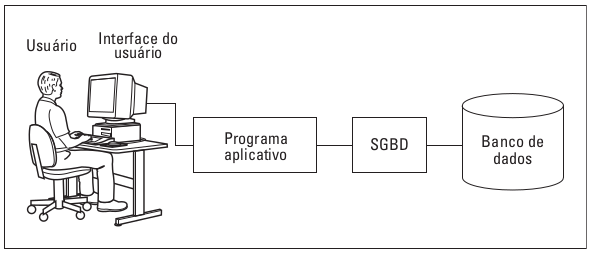
\includegraphics[width=1\hsize]{figuras/esquema_sgbd.png}
  %\legend{Texto da legenda quando necessário.}
  \source{\cite{taylor2016sql}}
\end{figure}
``Um sistema gerenciador de banco de dados (SGBD) é um
sistema de software genérico para manipular bancos de dados'' \cite[p.2]{teorey2014projeto}. Dessa forma, ``o principal objetivo de um SGBD é prover uma forma de armazenar e acessar informações de uma base de dados que seja ambos conveniente e eficiente'' \cite[p.1]{korth2010database}.

``Neste ponto, é importante evitar confundir o BD em si [..] com o programa que o gerenciará, o Sistema Gerenciador de Banco de Dados (SGBD). Em outras palavras, software como Access, MySQL, Oracle, PostgreSQL não são BD, mas sim SGBD'' \cite[p.2]{clickgeogeoprocessamento}.

%arquitetura de banco>DBA>SQL
Alguns autores divergem levemente na arquitetura de um SGBD. Adotando a linha de pensamento de \citeonline[p.12]{barcelarbanco}, a arquitetura de um SGBD pode se dividir em três níveis: \textit{nível externo}, \textit{nível conceitual} e \textit{nível físico}.
Nível externo é o nível em que o usuário `vê' o banco ou partes dele. O acesso do usuário delimita quais dados são visíveis à ele.
Nível conceitual é o nível onde se encontra o modelo conceitual do banco de dados. Neste modelo se define a estrutura de todo o banco, desde conceitos dos dados à como eles se relacionam. A estrutura neste momento é abstrata e não define o local físico de armazenamento. 
Nível físico (ou interno) define o esquema interno, onde é descrito detalhadamente os dados e o caminho de armazenamento dentro do servidor físico. 

Além da arquitetura existem dois conceitos importantes para um banco de dados: \textit{esquema} e \textit{instância}. De acordo com \citeonline[p.8]{korth2010database} em diferentes momentos o banco terá armazenado diferentes dados, estes momentos são chamados de instâncias. A estrutura onde se encontram esses dados é o esquema. Geralmente, enquanto a instância muda constantemente, o esquema raramente sofre mudanças.

Segundo \citeonline[p.22]{navathe2011fundamentals} é essencial para o funcionamento do SGBD uma elaboração cuidadosa do esquema do mesmo. Existe um tipo de dado, chamado \textit{metadado}, armazenado no catálogo do SGBD, também conhecido como dicionário de dados, que descreve as restrições e as construções do esquema, permitindo assim que o SGBD recorra aos metadados quando necessário.   
%[?]O modelo idealizado neste trabalho se encontra no nível conceitual, e o banco de dados resultante foi criado, testado e manuseado no nível externo.

%DBA
Trabalhando no nível conceitual está o administrador do banco de dado, conhecido como DBA. \citeonline[28-29]{korth2010database} afirma que o administrador possui várias funções, dentre elas, criação do banco de dados original, definir a estrutura de armazenamento, realizar modificações nas partes física e conceitual do modelo, garantir ou restringir acesso à outros usuários e o mesmo também é responsável pela manutenção de rotina do SGBD.%PERGUNTAR SE ESTAR CONCEITO ESTÁ CORRETO, POSSO ESTAR ENTENDENDO ERRADO O INGLÊS.

No nível externo se encontra o usuário comum. De acordo com \citeonline[p.12-13]{barcelarbanco} cada um dos usuários possui diferentes \textit{níveis de visão}. O usuário normal não tem visão total do esquema dos dados. O SGBD omite alguns detalhes desnecessários para o usuário de forma que o mesmo tenha um acesso rápido e eficiente aos dados. Essa omissão é feita através de \textit{níveis de abstração}.

\begin{citacao}
    Com o tempo, os SGBD’s passaram a utilizar diferentes formas de representação, ou modelos de dados, para descrever a estrutura das informações contidas em seus bancos de dados. Atualmente, os seguintes modelos de dados são normalmente utilizados pelos SGBD’s: modelo hierárquico, modelo em redes, modelo relacional (amplamente usado) e o modelo orientado a objetos. \cite[p.6]{takai2005intro}
\end{citacao}

Tendo em vista as necessidades deste trabalho, são apresentados os SGBDs baseados no modelo relacional, modelo orientado a objeto e modelo mais recente, modelo objeto-relacional. 

%SGBDR
%\subsubsection{Sistema Gerenciador de Banco de Dados Relacional}\label{sgbdr}
\subsubsection{Modelos de SGBDs}\label{sgbdr}

\begin{citacao}
    ``A abordagem relacional aos dados está baseada na observação de que arquivos que obedecem a certas limitações podem ser considerados como relações matemáticas, e consequentemente a teoria elementar de relações pode ser usada para lidar com vários problemas práticos dos dados desses arquivos'' \cite[p.77]{date1989introducao}.
\end{citacao}

Isso significa que ``o modelo relacional implementa estruturas de dados organizadas em relações'' \cite[p.8]{takai2005intro}. 
Porém antes de se se entender melhor essas `relações' deve-se mencionar que existe uma questão de inconsistência para a terminologia usada na literatura para o banco de dados. Isso se deve pelo seguinte motivo:

``A principal linguagem de manipulação de dados em sistemas de bancos de dados relacionais é o SQL'' \cite[p.9]{alexandruk2011modelagem}. Devido ao desenvolvimento e expansões ao longos dos anos o SQL foi `adaptado' e padronizado tanto pela ANSI quanto pela ISO, tornando a linguagem como padrão para banco de dados tanto relacionais quanto de outros tipos. Isso gera uma `confusão' dentre muitos usuários de banco de dados, principalmente relacionais, portanto deve-se ressaltar que ''SQL e o Modelo Relacional não são a mesma coisa'' \cite{date2011sql}.

A citação, a seguir, explica a estrutura de um banco de dados relacional e exemplifica a questão discutida acima sobre terminologia:
\begin{citacao}
    A estrutura fundamental do modelo relacional é a relação (tabela). Uma relação é constituída por um ou mais atributos (campos) que traduzem o tipo de dados a armazenar. Cada instância do esquema (linha) é chamada de tupla (registro) \cite[p.8]{takai2005intro}.
\end{citacao}


Percebe-se que o autor ao explicar as definições de `relação', `atributo', `instância de esquema' e `tupla' usa dois termos para cada definição. Enquanto exite terminologias mais comuns na literatura, cada autor usa em seus textos a de sua preferência. 

Para facilitar a compreensão deste trabalho, não se adotará uma terminologia específica, de forma que todo e qualquer termo utilizado será previamente ou posteriormente explicado. 

Voltando à explicação dada por \citeauthor{takai2005intro} acima, a figura \ref{tabelas_exe} ilustra um exemplo de dados em um SGBDR.  

\begin{figure}[!ht]{10cm}
  \caption{Exemplos de tabelas que podem ser armazenadas em um SGBDR} \label{tabelas_exe}
  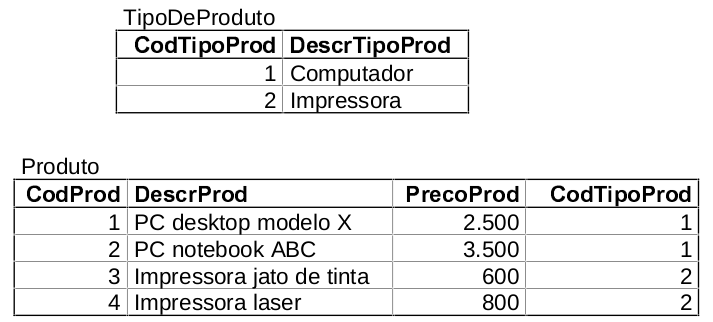
\includegraphics[width=1\hsize]{figuras/tabelas_exemplo.png}
  %\legend{Texto da legenda quando necessário.}
  \source{\cite{heuser1998projeto}}
\end{figure}

Na figura \ref{tabelas_exe} existem duas tabelas chamadas de `TipoDeProduto' e `Produto'. Na primeira tabela encontra-se dois atributos `CodTipoProd' e `DescrTipoProd' enquanto na segunda tabela tem-se `CodProd', `DescrProd', `PrecoProd' e `CodTipoProd' como atributos. Analisando ainda a figura \ref{tabelas_exe} percebe-se um padrão para cada atributo. Esse padrão é denominado \textit{domínio}. Pode-se supor que o domínio do atributo `CodProd' é do tipo `INT', o que significa que naquela tabela serão somente armazenados valores de números inteiros. Porém no atributo `DescrProd' o domínio pode ser do tipo `VARCHAR', que aceita valores textuais ou numéricos como texto com variação de 1 a 8000 bytes. Os tipos de domínios serão explorados mais a frente.

Contudo, existem dados mais complexos, como por exemplo geometrias localizadas no espaço geográfico, que o SGBDR não comporta. Para esses dados foi adotado outro método de modelagem, que utiliza não só os recursos básicos relacionais como também o SQL provido das extensões orientadas a objetos para suporte espacial necessárias. O SGBD de interesse para o trabalho será discutido no próximo item.

%\subsubsection{Sistema Gerenciador de Banco de Dados de Objetos} %PEDIR AO IRVING PARA CHECAR ESTE ITEM, ACHO QUE ESTA FALTANDO MENCIONAR ALGUMA COISA, OU DAR UMA EXPLICAÇÃO QUE ME PERMITA USAR UM TERMO ESPECÍFICO...
%Definição de um SGBDO
\citeonline[p.145]{teorey2014projeto} comenta que a modelagem orientada a objetos é uma forma de mapear o mundo real. 
\begin{citacao}
    A motivação para seu surgimento está em função dos limites de armazenamento e representação semântica impostas no modelo relacional. Alguns exemplos são os sistemas de informações geográficas (SIG)[..] O termo Modelo Orientado a Objetos é usado para documentar o padrão que contém a descrição geral das facilidades de um conjunto de linguagens de programação orientadas a objetos e a biblioteca de classes que pode formar a base para o Sistema de Banco de Dados. \cite[p.8-9]{alexandruk2011modelagem}
\end{citacao}

Em outras palavras, ``com tipos de sistemas complexos pode-se representar conceitos de modelos ER. Como atributos compostos, atributos multi-valorados, generalização, e especialização diretamente, sem a tradução complexa do modelo relacional'' \cite[p.947]{korth2010database}

``Um recurso dos bancos de dados de objeto é o poder que eles dão ao projetista para especificar tanto a \textit{estrutura} dos objetos complexos quanto as \textit{operações} que podem ser aplicadas a esses objetos'' \cite[p.236]{navathe2011fundamentals} 

Pensando na estrutura, segundo \citeonline[p.4]{alexandruk2011modelagem} o pensamento por trás da orientação a objeto em banco de dados consiste na concepção de herança entre os dados. Estes são tratados como dados abstratos, e portanto objetos. Na abstração ``a ideia básica é retirar os detalhes e reter exatamente o máximo da complexidade da vida real quanto for exigido para a tarefa em mãos'' \cite[p.142]{teorey2014projeto}.  Assim os dados podem ser agrupados como um único objeto, estruturando-os em classes e superclasses. Observa-se assim hierarquias, como demonstrado na figura \ref{heranca_obj}.

\begin{figure}[!ht]{10cm}
  \caption{Exemplo de herança na orientação objeto.} \label{heranca_obj}
  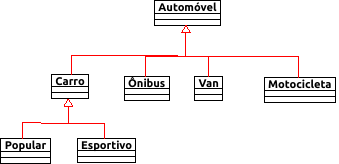
\includegraphics[width=1\hsize]{figuras/heranca.png}
  %\legend{Texto da legenda quando necessário.}
  \source{A autora}
\end{figure}

Analisando a figura \ref{heranca_obj} tem-se uma superclasse `Automóvel', que se subdivide em várias classes. Das classes `Carro', `Ônibus',`Van' e `Motocicleta', qualquer dado da classe `Carro' pode ser entendida como do tipo subclasse `Popular' ou `Esportivo'.  De forma simples, isso significa que na herança, para cada entrada de dado, existirá atributos em comum dentre os objetos dessa herança. Todo registro na entidade `Popular' terá também dados complementares relacionados a esse registro transcritos no objeto `Carro' e, num nível acima, no objeto `Automóvel'. 

Esse tipo de distinção entre os dados como objeto não seria possível em um banco de dados relacional, pois de acordo com \citeonline[p.4]{alexandruk2011modelagem}, as relações de um banco só possuíam valores atômicos até então.
Se `Automóvel', da figura \ref{heranca_obj}, fosse aplicado em um banco de dados relacional, esta superclasse seria uma tabela com dúzias de atributos com muitos deles possuindo dados repetidos para poder simplesmente armazenar um tupla. Isso afeta a eficiência com a qual o banco acessa os dados dessa tabela.

Como este trabalho é voltado para, entre outros, dados geográficos, no item \ref{ext_geo} será comentado superficialmente sobre extensões geográficas que são aceitas como padrão\footnote{Seguindo a especificação OpenGIS\cite{opengis}} para os SGBDs que implementem esses tipos de dados complexos. 


%qual a diferença entre um SGBDR e um SGBDO?

%\subsubsection{Sistema Gerenciador de Banco de Dados Objeto Relacional}
%SGBDOR (não preciso entrar a fundo nisso, pois ao explicar SGBDR e SGBO eu ja mato o assunto)

Segundo \citeonline[p.15-18]{navathe2011fundamentals} dados complexos, como os dados geográficos não são atendidos pelo banco de dados relacional devido às suas características. Porém os mesmos, como comentado anteriormente, podem ser modelados de acordo com a estrutura de um banco de dados orientado a objeto. 

Assim sendo, devido a sua simplicidade, existe uma preferência ao SGBDR no mercado em comparação ao SGBDO, ``muitos conceitos orientados a objeto foram incorporados nas versões mais recentes do SGBD relacional, levando a sistemas de gerenciamento de banco de dados objeto-relacional, conhecidos como SGBDORs'' \cite[p.16]{navathe2011fundamentals}.
\begin{citacao}
    Esses sistemas [...] implementam uma camada de abstração de dados em cima de métodos relacionais, o que torna possível a manipulação de dados mais complexos. [...] Todas as características relacionais permanecem, ou seja, as tabelas continuam a existir, porém elas possuem alguns recursos adicionais.\cite[p.4]{alexandruk2011modelagem}.
\end{citacao}

\subsubsection{Extensões Geográficas}\label{ext_geo}
%Qual o diferencial da informação geográfica? 
``Modelos de dados para aplicações geográficas têm necessidades adicionais, tanto com relação à abstração de conceitos e entidades, quanto ao tipo de entidades representáveis e seu inter-relacionamento'' \cite[p.86]{borges2005modelagem}. Em outras palavras,``a modelagem de dados geográficos é uma atividade complexa porque envolve a discretização do espaço como parte do processo de abstração, visando obter representações adequadas aos fenômenos geográficos'' \cite[p.30]{queiroz2006tutorial}.


De acordo com \citeonline[p.358-359]{guting1994an} bancos de dados espaciais proveem a tecnologia básica para aplicações como Sistemas de Informação Geográficos - SIG (em inglês Geographic Information System - GIS). Eles devem três características básicas. 
\begin{itemize}
    \item Bancos de dados espaciais devem ser também bancos de dados, pois todo dado espacial se relaciona de alguma forma com dados alfanuméricos. Isso implica no banco ter capacidade de lidar com esse tipo de dado além do espacial.
    \item Deve oferecer tipos específicos de `data type' que atendam as características espaciais no modelo de dados e na linguagem de consulta. Esse `data type' determina o domínio do atributo, assim permitindo que o banco trabalhe com os dados geométricos relacionados ao terreno, da mesma forma que suas relações.
    \item Fornecer indexação espacial e algoritmos voltados para o tratamento desses dados, de forma que o sistema seja capaz de obter uma coleção de objetos de um conjunto de dados presentes num terreno. Eles devem também ser capaz de conectar objetos de diferentes classes por seus dados espaciais.
\end{itemize}

``No que se refere ao ramo de banco de dados (BD) com extensões geográficas os nomes mais citados em debates em geral são Oracle Spatial, PostgreSQL/PostGIS e MySQL Spatial'' \cite[P.1]{clickgeosgbd}

\subsection{Processo de Desenvolvimento de Sistemas} \label{proc}

\begin{citacao}
Método é um procedimento ou técnica utilizado para obter um determinado resultado. Também pode ser definido como uma forma de agir em uma determinada situação a fim de regularizar uma tarefa. Com essa definição é possível entender o porquê é fácil encontrar várias metodologias para o desenvolvimento de documentação de software. Isso acontece porque são vários os tipos de software que são desenvolvidos em várias linguagens para diversos ambientes e desenvolvidos em diversos modelos de sistemas de informação, tais como baseado em fluxo de dados, relacionais e orientado a objetos. \cite[p.402]{keila2010metodologias}
 \end{citacao}
 
De acordo com \citeonline[p.2-3]{dos2004comparaccao} existem metodologias tradicionais e metodologias ágeis. Pode-se entender como modelo sequencial, que é um modelo tradicional,  aquele onde cada etapa deve ser finalizada antes de outra ser iniciada, ou seja, deve seguir uma sequência, apresentado inicialmente no modelo de Royce. O modelo de cascata, como ilustrado na figura \ref{waterfall}, é um exemplo de modelo sequencial.

\begin{figure}[!ht]{10cm}
  \caption{Ilustração do modelo em cascata.} \label{waterfall}
  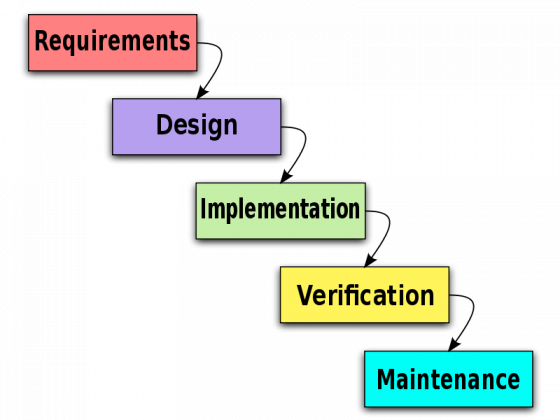
\includegraphics[width=0.6\hsize]{figuras/Waterfall-Model-560x420.png}
  \source{\cite{tech2019waterfall}}
\end{figure}

Onde os termos `Requirements', `Design', `Implementation', `Verification' e `Maintenance' podem ser entendidos de forma geral como as etapas de um processo de desenvolvimento de sistemas. Assim se referem respectivamente a: a definição de requisitos, projeto do software, implementação e teste unitário, integração e teste do sistema, operação e manutenção. 
Segundo \citeonline[p.2]{tech2019waterfall} um modelo monolítico, como o apresentado, possui uma grande desvantagem: pouca, se não inexistente, maleabilidade que comporte mudanças ocorridas ao longo do processo. Desta forma, \citeonline[p.4]{badolato2019} afirma que se houver necessidade de mudanças durante o processo com este modelo, todo o trabalho realizado até aquele ponto é perdido. Em suma, a expectativa de reaproveitar o trabalho nos leva à reflexão de como adaptar o modelo para ser capaz de lidar com mudanças.

Uma forma de se resolver este problema foi a integração de componentes, ilustrada na figura \ref{integracao}. Desta forma o processo é subdividido em partes com cada parte sendo trabalhada individualmente. Assim acarretando numa retro-alimentação, também conhecida como incremental. Este modelo de processo continua sendo monolítico, porém agora existe uma maior maleabilidade ao longo do desenvolvimento.

\begin{figure}[!ht]{15cm}
  \caption{Modelo de processo incremental.} \label{integracao}
  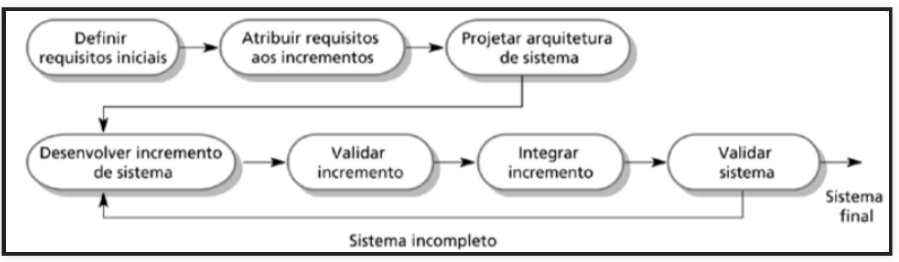
\includegraphics[width=1\hsize]{figuras/integracao.png}
  %\legend{Texto da legenda quando necessário.}
  \source{\apud{sommerville2008engenharia}{badolato2019}}
\end{figure}

Neste caso, os requisitos iniciais são identificados, atribuídos aos incrementos, como uma lista de atividades, e geram então uma visão macro da arquitetura do projeto. A partir daí cada incremento é trabalhado separadamente, enquanto ocorre a retro-alimentação e consequente revisita das atividades do processo. Segundo ainda \citeonline{badolato2019} a alteração pela simples adição de retroalimentação no processo modelado na figura \ref{waterfall}, enquanto trata das mudanças, não apresenta solução para o problema do tempo gasto quando os projetos são demasiadamente grandes, o que incide no atraso da entrega do sistema em face ao prazo. 

O atraso na entrega do sistema pode gerar `tensão' entre o implementador e o cliente. Visando solucionar este problema, a abordagem se torna ``em espiral'', na qual o produto é quebrado em pequenos componentes, que são incorporados ao produto e entregues ao cliente a medida que são finalizados. Esta abordagem enquanto mais rápida pode ser também rígida e complexa.

Tomando por base o modelo em espiral, existe ainda a necessidade de uma padronização do processo de desenvolvimento de software, onde a interação é dinâmica, fato que levou ao modelo denominado ``ágil''.

\begin{citacao}
O termo “Metodologias Ágeis” tornou-se popular em 2001 quando dezessete especialistas em processos de desenvolvimento de software representando os métodos Scrum [Schwaber e Beedle (2002)], Extreme Programming (XP) [Beck (1999)] e outros, estabeleceram princípios comuns compartilhados por todos esses métodos.\cite[p.3]{dos2004comparaccao}
\end{citacao}

O modelo ágil, diferentemente do tradicional, é cíclico. Isso permite que os requisitos estabelecidos inicialmente sejam modificados de acordo com a evolução do desenvolvimento do sistema. A implementação também faz parte de cada ciclo, diferentemente do modelo monolítico onde antes a implementação só ocorria em um momento avançado do desenvolvimento. A tabela \ref{agil_trad} exibe as principais diferenças entre o modelo tradicional (monolítico) e o modelo ágil (cíclico).

\begin{table}[!ht]{14cm}
  \caption{Comparação entre modelo Ágil e Modelo Tradicional.}\label{agil_trad}
    \begin{tabular}{cc}
    \hline
    \rowcolor[HTML]{333333} 
    {\color[HTML]{FFFFFF} \textbf{Modelo Ágil}} & {\color[HTML]{FFFFFF} \textbf{Modelo Tradicional}} \\ \hline
    \rowcolor[HTML]{EFEFEF} 
    \begin{tabular}[c]{@{}c@{}}Abordagem iterativa, permitindo que \\ ocorram mudanças durante todo o \\ processo\end{tabular} & \begin{tabular}[c]{@{}c@{}}Abordagem sequencial, cada, etapa é \\ fechada e precisa ser finalizada antes \\ do inicio na etapa seguinte\end{tabular} \\
    \begin{tabular}[c]{@{}c@{}}Funciona bem quando o projeto não \\ é conhecido\end{tabular} & \begin{tabular}[c]{@{}c@{}}Atende melhor quando se sabe o \\ projeto\end{tabular} \\
    \rowcolor[HTML]{EFEFEF} 
    \begin{tabular}[c]{@{}c@{}}É importante ter acesso ao cliente \\ durante todo o processo\end{tabular} & \begin{tabular}[c]{@{}c@{}}O cliente só é consultado no início e \\ posteriormente na entrega do software\end{tabular} \\
    \begin{tabular}[c]{@{}c@{}}Permite verificações e validações \\ preliminares, aumentando as chances \\ de sucesso no programa final\end{tabular} & \begin{tabular}[c]{@{}c@{}}Não permite validações ou verificações \\ durante, processo, diminuindo as \\ chances de sucesso ao final do processo\end{tabular} \\
    \rowcolor[HTML]{EFEFEF} 
    \begin{tabular}[c]{@{}c@{}}Software é exaustivamente testado \\ durante todo o processo\end{tabular} & \begin{tabular}[c]{@{}c@{}}Teste só pode ser realizado ao final do \\ processo\end{tabular} \\
    \begin{tabular}[c]{@{}c@{}}O implementador tem total flexibilidade \\ dentro dos parâmetros do programa\end{tabular} & \begin{tabular}[c]{@{}c@{}}O implementador fica preso a \\ documentação inicial e tem pouca \\ flexibilidade no desenvolvimento \\ do sistema\end{tabular} \\ \hline
    \end{tabular}
  \source{A autora.}
\end{table}


Existem muitas práticas usadas na atualidade em conjunto com os modelos ágeis para desenvolvimento de um sistema.

Um exemplo de prática Ágil é o Test Driven Development (TDD). De forma resumida pode-se dizer que o TDD consiste no teste e erro. Num primeiro momento o desenvolvedor escreve o suficiente do código para testa-lo. Em seguida realiza esse teste com a expectativa de falhar (1) para evidenciar que o teste é suficientemente crítico. Em seguida o código deve ser consertado a ponto de passar no teste já estabelecido (2). Posteriormente o código deve sofrer alterações e incrementos de forma a ser melhorado (3). Ao final dessa etapa o código deve ser novamente testado com a perspectiva de falhar, logo voltando a etapa inicial para ser capaz de tratar limites, exceções ou novos problemas não abordados nas iterações iniciais. A imagem \ref{TDD} ilustra o fluxograma de um TDD.

\begin{figure}[!ht]{10cm}
  \caption{Fluxograma do TDD.} \label{TDD}
  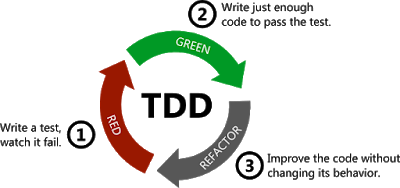
\includegraphics[width=0.75\hsize]{figuras/tdd_flow.png}
  %\legend{Texto da legenda quando necessário.}
  \source{\cite{chairat2017}}
\end{figure}

``A pequena granularidade do ciclo test-then-code dá um feedback contínuo ao programador. Falhas são identificadas mais rapidamente, enquanto o novo código é
adicionado ao sistema. Assim, o tempo de depuração diminui compensado pelo tempo de escrita e execução dos casos de teste'' \cite[p.4]{borges2006conceitos}

Um problema comum neste método é a forma de raciocinar do implementador. Utilizando esta prática ágil não se começa com um código completo, mas sim com um pequeno pedaço dele, que a partir destes testes cresce até atingir os objetivos estabelecidos pelo desenvolvedor. 

O RUP (Rational Unified Process), que é um exemplo de processo moderno baseado na UML e será apresentado posteriormente no item \ref{itemmodl}, foi criado pela mesmo grupo responsável pela criação da UML. Enquanto o modelo não é usado diretamente no trabalho, ele expõem conceitos relacionados à evolução da apresentado pelas metodologias ágeis. A figura \ref{RUP} apresenta o modelo RUP.

\begin{figure}[!ht]{10cm}
  \caption{RUP - Rational Unified Process.} \label{RUP}
  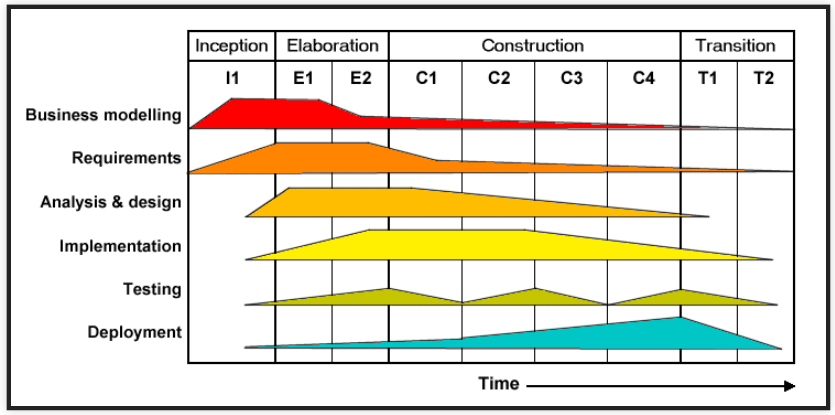
\includegraphics[width=1\hsize]{figuras/rup.png}
  %\legend{Texto da legenda quando necessário.}
  \source{\apud{RUP}{badolato2019b}}
\end{figure}

Analisando a figura \ref{RUP} percebe-se uma distribuição do esforço no desenvolvimento das atividades de cada uma das fases do processo. A um primeiro momento se tem maior esforço atribuído às atividades de definição das regras do negócio e o levantamento dos requisitos, mais a frente durante a fase de elaboração o foco leva a um maior esforço para análise e projeto, durante a construção percebe-se uma carga maior para as atividades de elaboração e teste, sendo que este último está presente durante todo o processo, tendo `picos' ao final de marcos nos quais novos componentes foram construídos e precisam ser aprovados para viabilizar sua entrega. Por último tem-se a aplicação/entrega do sistema que cresce a medida em que as fases finais do processo se aproximam.



\subsection{Conceito de Requisitos de Sistemas} \label{conceitos_requisitos}
Segundo \citeonline[p.3-5]{teorey2014projeto} o primeiro procedimento na elaboração de um banco de dados é a \textit{análise de requisitos}. Parte fundamental do esquema conceitual, os requisitos são especificados a partir de encontros entre o desenvolvedor do banco de dados e o cliente. As informações colhidas dessa reunião geram os requisitos que servirão para restringir e modelar o banco no nível abstrato. Sabendo que ``o esquema conceitual tem como objetivo servir como uma fundação sólida e duradora para a operação global da empresa'' \cite[p.425]{date2011sql}, fica fácil entender que os requisitos são fundamentais para todo o processo de desenvolvimento do sistema.  

De acordo com \citeonline[p.3]{badolato2019b} a primeira coisa a ser feita é o \textit{estudo de viabilidade}.
O estudo de viabilidade pode ser considerado uma etapa 'pré-projeto', onde se pesquisa quais são os possíveis problemas a serem encontrados durante a realização do processo e quais possíveis formas de solucionar esses problemas. Logo em seguida vem a etapa de \textit{elicitação e análise}.

A elicitação e análise de requisitos, é um detalhamento do projeto que ocorre assim que o mesmo é iniciado. Segundo \citeonline[p.14-20]{souza2014banco}, o problema é identificado por meio de perguntas simples, assim estabelecendo: 
\begin{itemize}
    \item uma ideia básica do problema;
    \item quem é afetado de fato por esse problema;
    \item qual é ideia geral por trás da solução planejada;
    \item uma comunicação eficiente entre o produtor e o cliente.
\end{itemize}
Obviamente as perguntas iniciais definem o problema em escopo geral. Segundo esse mesmo autor, para elicitar os requisitos, logo identificar o problema, existem várias técnicas. Dentre elas: amostragem, investigação, entrevista, observação, elaboração de questionários, prototipação etc. 
Neste trabalho a elicitação dos requisitos foi realizada por meio de \textit{brainstorm}.

\textit{Brainstorming} é uma
\begin{citacao}
 ferramenta para geração de novas ideias sobre um determinado assunto. A técnica deve ser livre de críticas que inibam a contribuição dos participantes. O foco é a geração de ideias que podem estar relacionadas às causas, modos de abordagem ou ações a serem tomadas sobre determinado assunto.\cite[p.7]{subplan2014}
\end{citacao}

De acordo com \citeonline[p.109]{leffingwell2000managing}, \textit{brainstorm} possui dois objetivos, a geração e redução de ideias. Primeiro ocorre a exposição de ideias pelos participantes da \textit{brainstorm} e depois essas ideias são reduzidas por meio de organização, catalogação, expurgo de duplicatas etc.

No levantamento de requisitos isso implica em uma ou mais reuniões entre produtor e cliente onde o problema é apresentado pelo cliente. O produtor então pergunta sobre esse problema e expõem possíveis soluções para o mesmo. Durante uma \textit{brainstorm} o problema e as soluções são escritas em um local qualquer, desde um quadro a folhas de papel, assim provendo por essas anotações uma forma de ambas as partes acompanharem o segmento de ideias expostas.

Após a elicitação e análise, \citeonline[p.3]{badolato2019b} define que deve ocorrer a \textit{especificação dos requisitos}.

De acordo com \citeonline[p.24-25]{souza2014banco} a especificação dos requisitos é a formalização do que será feito, ou seja, ocorre a descrição de como o sistema vai se comportar para atender os requisitos levantados por meio de uma documentação. Seja ela um documento simples, um modelo de gráfico, um modelo formal matemático etc, que defina de forma estruturada e detalhada os requisitos e como eles se relacionam. Essa etapa é revisitada ao final do processo para orientar a validação do produto.

A figura \ref{faseteste} esquematiza as etapas a serem tomadas pelo desenvolvedor, necessárias para a criação do sistema.

\begin{figure}[!ht]{13cm}
  \caption{Planejamento e execução de testes entre as etapas de criação do sistema.} \label{faseteste}
  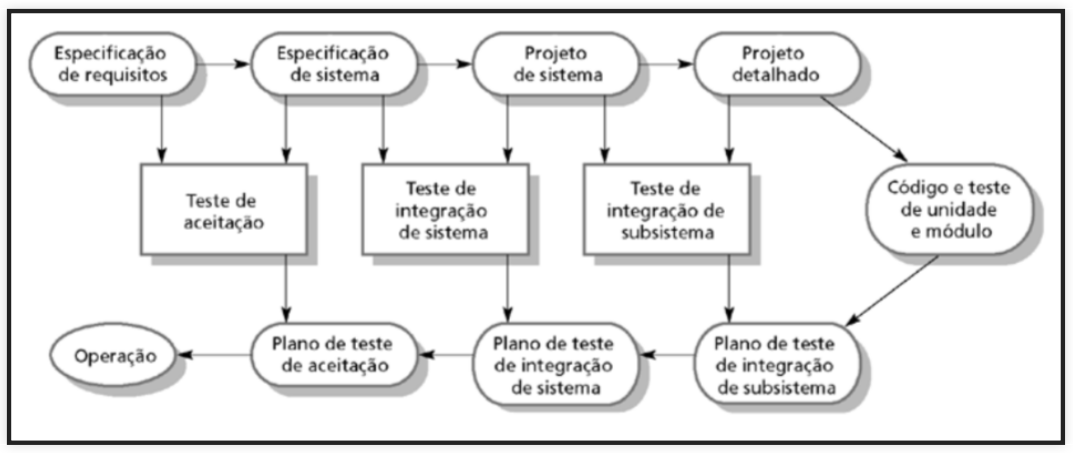
\includegraphics[width=1\hsize]{figuras/fases_de_teste.png}
  %\legend{Texto da legenda quando necessário.}
  \source{\cite{sommerville2013engenharia}}
\end{figure}

Como podemos ver analisando a figura \ref{faseteste} há relacionamento entre as atividades iniciais e finais do processo, isto é, requisitos e decisões de projeto geram os insumos para testes do sistema após sua implementação. Observa-se na figura que, em um primeiro momento, ocorre a `especificação dos requisitos'. Esta, por sua vez, gera com esses requisitos a `especificação do sistema'. Em seguida, ocorre a etapa denominada 'projeto do sistema', que é a criação do sistema num nível macro. O projeto então é detalhado, o que permite a realização da etapa  `codificação e testes de unidade e módulo'. Neste momento iniciam-se as etapas de verificação com o `plano de teste de integração de sistemas' e o `plano de teste de integração de subsistemas'. Nessas duas fases o sistema está sendo integrado, ou seja, primeiro são testadas as partes menores e depois como elas se comunicam. Por último ocorre a validação presente no `plano de teste de aceitação'.

Segundo \citeonline[p.27-28]{sommerville2013engenharia}, existem três processos de teste a serem realizados para obter-se a validação e verificação de um sistema. \textit{Testes de desenvolvimento} são testes realizados em componentes do sistema (entidades simples, classes de objetos etc.). \textit{Testes de sistema} por outro lado, testam o sistema como um todo, focando na iteração entre os componentes do sistema. Por fim, os \textit{testes de aceitação} são testes realizados com dados fornecidos
pelo cliente, que podem identificar erros no sistema ou até mesmo problemas nos requisitos levantados. Os testes de aceitação fazem parte do estágio final do processo de desenvolvimento, e são eles os responsáveis pela validação do sistema. \citeauthoronline{sommerville2013engenharia} afirma também que em uma abordagem incremental cada incremento é testado ao longo de seu desenvolvimento.
Para a figura \ref{faseteste} isso significa que em paralelo são produzidas e realizadas as etapas `teste de aceitação', `teste de integração do sistema', que testa o sistema' como um todo e `teste de integração de subsistema' que testa as partições desse sistema.



Até o presente momento foi falado sobre `verificação' e `validação' sem defini-las. Porém existe uma distinção entre ambas definida pela literatura. Em termos simples, a verificação se preocupa com o funcionamento do sistema de acordo com as técnicas utilizadas. A validação, por outro lado, se refere ao fato de o programa atender os objetivos do implementador, ou seja, atender aos requisitos identificados no início do processo. Isso significa que em algum momento durante o processo de desenvolvimento, o sistema deve ser verificado e validado. 

\begin{figure}[!ht]{10cm}
  \caption{Resumo do processo de desenvolvimento de sistema.} \label{verval}
  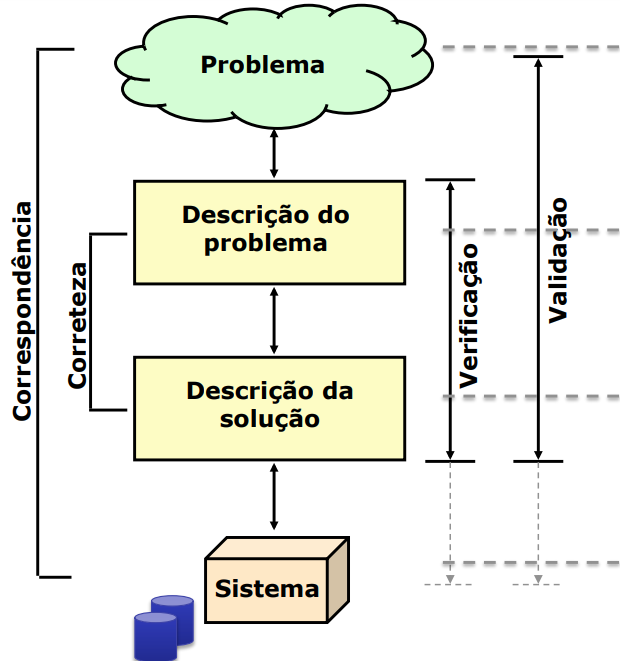
\includegraphics[width=0.5\hsize]{figuras/requisito_proj_proc.png}
  %\legend{Texto da legenda quando necessário.}
  \source{\cite{souza2014banco}}
\end{figure}

A figura \ref{verval} ilustra de forma resumida e simples o assunto descrito nos parágrafos anteriores. Analisando-a entende-se que primeiramente existe um problema a ser trabalhado. O mesmo precisa ser descrito, ou seja, seus requisitos são identificados. A partir dessa descrição é proposta uma solução, que descreve como esses requisitos se comunicam. Assim, da solução proposta se implementa um sistema. O sistema deve atender todas as expectativas levantadas de acordo com o problema identificado para poder ser validado. Já a solução proposta para o problema deve funcionar segundo as técnicas da linguagem utilizada de forma que a solução então possa ser considerada verificada. No capítulo \ref{results} será apresentado como a validação do projeto piloto foi realizada.

Por último, \citeonline{badolato2019b} afirma que deve-se entender que os requisitos podem ser de dois tipos: \textit{requisitos de sistemas} e \textit{requisitos de usuários}.
%definição:
Requisitos de usuários são a descrição, em linguagem natural, em um documento das restrições do sistema com foco no usuário comum, sem grandes conhecimentos computacionais, o cliente.

Requisitos do sistema são requisitos definidos para os subsistemas, que não necessariamente estão descritos segundo os termos do negócio do cliente. Neste caso o documento gerado tem como foco os requisitos implementados do programa ou do banco.

Ao final deste item pode-se concluir que a comunicação entre cliente e equipe de desenvolvimento é essencial para a identificação dos requisitos que permitem o produto final atender as expectativas do cliente, o que implica na validação do produto. A figura \ref{comunicado} exemplifica quando essa comunicação não é eficiente.

\begin{figure}[!ht]{10cm}
  \caption{Ilustração de situação na qual não ocorre uma comunicação eficiente entre cliente e desenvolvedor.} \label{comunicado}
  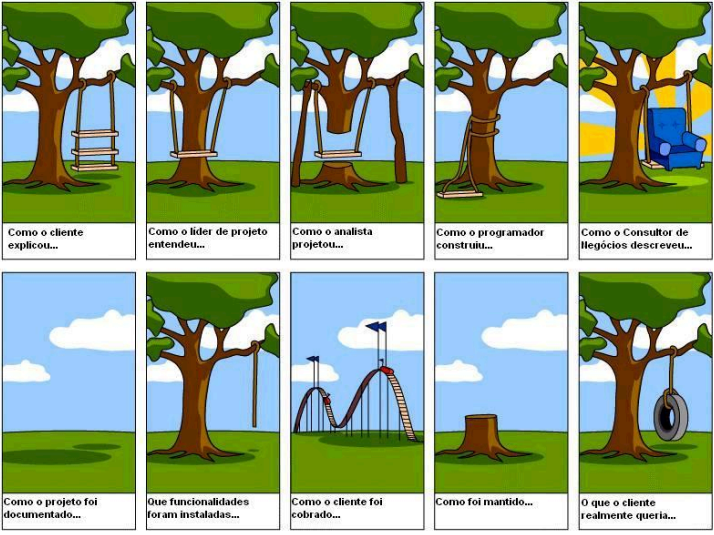
\includegraphics[width=1\hsize]{figuras/requisitos_malcomunicados.png}
  %\legend{Texto da legenda quando necessário.}
  \source{\cite{souza2014banco}}
\end{figure}

\subsection{Linguagens de Modelagem} \label{itemmodl}

\begin{citacao}
``O processo de modelagem conceitual de banco de dados compreende a descrição dos possíveis conteúdos dos dados, além de estruturas e de regras a eles aplicáveis. Essa descrição do banco de dados é feita com base nos construtores semânticos fornecidos por um modelo conceitual'' \cite[p.20]{lisboa2001modelagem}. 
\end{citacao}

Todo modelo trabalha com uma linguagem de modelagem, esta por sua vez ``pode ser composta de pseudo-código, código real, figuras, diagramas ou longas passagens de descrição; na verdade, é praticamente tudo o que ajuda
você a descrever seu sistema. Os elementos que compõem uma linguagem de modelagem são chamados
de notações'' \cite[p.2]{miles2006learning}.

Como apresentado anteriormente no item \ref{sgbdeg}, os tipos de dados a serem armazenados influenciam na escolha tipo de banco de dados, seu modelo e por consequência sua linguagem. Este trabalho tem como foco o acervo de dados do LFSR, constituído principalmente de materiais usados nos projetos de fotogrametria aérea tradicional, o que implica em dados geográficos e seus dados alfanuméricos. Sendo assim, neste item será apresentado algumas das particularidades dos dados geográficos que influenciam na modelagem e as linguagens de modelagem trabalhadas neste trabalho.

\begin{citacao}
    Entende-se por atributo qualquer informação descritiva (nomes, números, tabelas e textos) relacionada com um único objeto, elemento, entidade gráfica ou um conjunto deles, que caracteriza um dado fenômeno geográfico. Nos bancos de dados geográficos, os atributos de objetos geográficos são armazenados em relações convencionais. As representações geométricas destes objetos podem ser armazenadas na mesma tabela que os atributos ou em tabelas separadas, mas ligadas por identificadores únicos.\cite[p.30]{queiroz2006tutorial} 
\end{citacao}
De acordo com \citeonline[p.83-87]{borges2005modelagem}, na modelagem ocorre uma \textit{abstração} de objetos e fenômenos do mundo real assim representando-o, mesmo que de forma simplificada, dentro de um banco de dados. Para os autores a abstração dos conceitos e entidades do mundo real é fundamental na criação de um sistema de informação pois implica na qualidade da tradução dos dados e interações dos objetos desse mundo real para o meio digital. Essa modelagem é demasiada complexa pois envolve a \textit{discretização} do mundo real como parte do processo de abstração, tendo como objetivo uma representação clara dos dados geográficos e seus fenômenos. Existem vários níveis de abstração dos dados geográficos que influenciam no tipo de modelo adotado. São eles:

\begin{itemize}
    \item \textit{Nível do mundo real:} composto pelo objetos geográficos a serem representados. Ex.: rios, estradas, vilas, cidades, vegetação etc.
    \item \textit{Nível conceitual:} usa de um alto nível de abstração. Conceitua formalmente os objetos geográficos a serem modelados determinando as classes contínuas e discretas que entrarão no banco de dados.
    \item \textit{Nível de representação:} neste nível os objetos conceituados do nível conceitual são associadas a classes espaciais, variando de acordo com características como a escala, a projeção ou a visão do usuário. Este nível não possui semelhante no banco de dados tradicional, pois as aplicações tradicionais dificilmente lidam   com a questão da múltipla representação de camadas.
    \item \textit{Nível de implementação:} Define todos os parâmetros necessários para a implementação de forma que respeite os tipos de representações estabelecidos.
\end{itemize}
\begin{figure}[!ht]{10cm}
  \caption{Níveis de especificação de aplicações geográficas.} \label{apli_geo}
  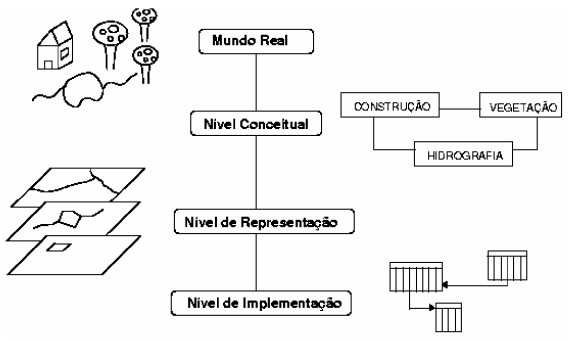
\includegraphics[width=1\hsize]{figuras/apl_geo.png}
  %\legend{Texto da legenda quando necessário.}
  \source{\cite{borges2002modelagem}}
\end{figure}

Corroborando com o explicado acima, \citeonline[p.12-16]{queiroz2006tutorial} afirmam que para a escolha do modelo é necessário se ter uma ideia do conceito de \textit{espaço absoluto} e \textit{espaço relativo}. 

A figura \ref{sao_paulo} exemplifica estes conceitos. Do lado esquerdo aparece um estado onde seus limites geográficos possuem valores de coordenadas correspondentes às estabelecidas na legislação, assim representando o espaço absoluto. Ao lado direito aparece um grafo das conexões entre distritos sobre este mesmo mapa, em forma de rede. No grafo as coordenadas exatas dos distritos não são armazenadas, assim caracterizando essa rede como um modelo de espaço relativo.
No espaço absoluto se encontram os geo-campos e geo-objetos, enquanto o espaço relativo possui o modelo de rede. 

\begin{figure}[!ht]{10cm}
  \caption{Exemplificação de espaço absoluto e espaço relativo.} \label{sao_paulo}
  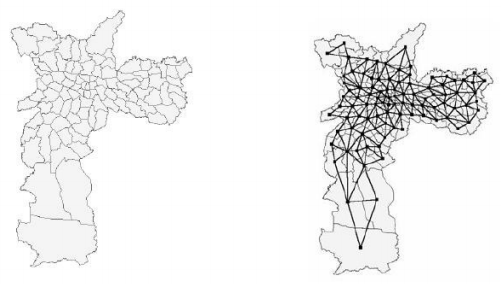
\includegraphics[width=0.75\hsize]{figuras/sao_paulo.png}
  %\legend{Texto da legenda quando necessário.}
  \source{\cite{queiroz2006tutorial}}
\end{figure}


Modelos de geo-campos são normalmente associados aos dados de tipo \textit{raster}. O modelo percebe o espaço geográfico como uma superfície contínua onde observa-se a variação de fenômenos. 
Assim, geo-campos dependem de suas definições físicas no terreno, de forma que se ocorrer uma partição genérica de um geo-campo, o geo-campo resultante possuirá as mesmas propriedades.

Já os modelos de geo-objetos entendem o espaço geográfico como um conjunto de entidades distintas e identificáveis, onde cada entidade possui um fronteira bem definida. Esse modelo normalmente é associado aos dados vetoriais.
Geo-objetos são entidades indivisíveis e singulares, que tem como caraterísticas suas individualidade, fronteiras e atributo. No caso de uma partição genérica, para o conjunto de geo-objetos gerado não estão garantidas as mesmas propriedades que o geo-objeto original.

Já o modelo de rede enxerga o espaço geográfico como um conjunto pontos (entidades), chamados de nós, que se comunicam por linhas, também chamados de arcos. Este modelo é normalmente relacionado a fluxos de transição, linhas de comunicação e acessibilidade etc. Os nós da rede são abstrações das entidades identificadas no terreno, onde as mesmas podem se relacionar de acordo com seus atributos descritivos.

\citeonline[p.21]{lisboa2001modelagem} afirmam que ``um modelo conceitual de dados deve prover construtores especiais para modelar tanto os campos quanto os objetos geográficos. A maioria dos modelos existentes não
suporta a modelagem dos fenômenos geográficos que são percebidos na visão de campo.''

De acordo com \citeonline[p.17] {queiroz2006tutorial} os conceitos apresentados podem ser aglomerados em um conceito genérico chamado de \textit{plano de informação}. Se forem adicionadas as subdivisões de geo-campo: \textit{geo-campo temático}, relacionado a medidas nominais ou racionais, e \textit{geo-campo numérico}, relacionados a medidas de intervalos ou razão, pode-se esquematizar um modelo orientado a objeto que serve como base para dados geográficos. Este esquema é demonstrado na figura \ref{oo_dados_geo}.

\begin{figure}[!ht]{14cm}
  \caption{Modelo orientado a objeto básico para dados geográficos} \label{oo_dados_geo}
  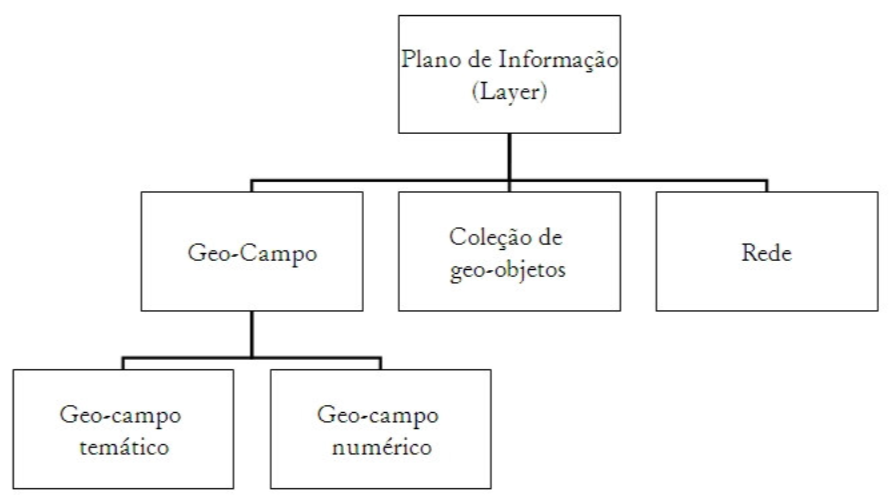
\includegraphics[width=0.75\hsize]{figuras/oo_dados_geo.png}
  %\legend{Texto da legenda quando necessário.}
  \source{\cite{queiroz2006tutorial}}
\end{figure}

Este modelo é facilmente identificado como base para muitos modelos orientados a objetos usados na geo-informação. Como por exemplo os modelos utilizados pelos programas SPRING, ArcGIS, GGIS e TerraLib. 

Segundo \citeonline[p.86]{borges2005modelagem}, existem muitas propostas de extensões para linguagens de modelagem voltadas a aplicações tradicionais de forma a atender as necessidades das aplicações geográficas. São exemplos destas extensões: GeoFrame e OMT-G.

Pode-se definir que
\begin{citacao}
    GeoFrame é um framework conceitual [...], baseado no paradigma de orientação a objetos, para ser usado na modelagem conceitual de bancos de dados geográficos. Este framework utiliza as notações e conceitos da linguagem UML. O objetivo de um framework conceitual é fornecer um conjunto de classes genéricas para um determinado domínio de aplicação para ser usadas como base ou molde para modelar aplicações específicas dentro desse domínio. O produto final de um framework conceitual é um esquema conceitual de dados. \cite[p.43]{queiroz2006tutorial}
\end{citacao}

O modelo OMT-G também é baseado na linguagem UML 
\begin{citacao}
    introduzindo primitivas geográficas com o objetivo de aumentar a capacidade de representação semântica daquele modelo e, portanto reduzindo a distância entre o modelo mental do espaço a ser modelado e o modelo de representação usual. [...] o modelo permite a especificação de atributos alfanuméricos e métodos associados para cada classe. Os principais pontos do modelo são sua expressividade gráfica e sua capacidade de codificação, uma vez que anotações textuais são substituídas pelo desenho de relacionamentos explícitos, que denotam a dinâmica da interação entre os diversos objetos espaciais e não espaciais.\cite[p.88]{borges2005modelagem}
\end{citacao}

Percebe-se que ambos os modelos se baseiam na linguagem UML. Devido à questão de acesso às ferramentas de implementação destes modelos foi decidido trabalhar diretamente com a UML 2.0. Enquanto esta por sua vez não é perfeita para modelagem de dados geográficos, como demonstrado pela existência de extensões propostas do modelo GeoFrame e do modelo OMT-G, estima-se que a linguagem UML 2.0 consegue atender as necessidades de modelagem do banco de dados deste trabalho de forma satisfatória.

\subsubsection{Unified Modeling Language - UML}\label{uml2.0}
\citeonline[p.5-8]{miles2006learning} explica que existe diferenças entre linguagens formais e linguagens informais. A linguagem informal normalmente não possui notações bem definidas. São suscetíveis a ambiguidades, o que leva por sua vez à modelagem equivocada de um conjunto de dados. Outro fator importante é que pela falta de precisão, uma linguagem informal não pode ser codificada. Para evitar esses e outros problemas que se opta por uma linguagem formal.

``A Linguagem de Modelagem Unificada (UML) emergiu como notação diagramática padrão para a modelagem orientada a objetos'' \cite[p.9]{silva2007introuml}. Esta afirmação é corroborada por \citeauthoronline{takai2005intro} quando o mesmo fala que ``o diagrama de classes UML serve geralmente como o esquema para o modelo de dados orientado a objetos'' \cite[p.9]{takai2005intro}.

Segundo \citeonline[p.10-13]{silva2007introuml} e (\citeyear{silva2007classesuml}, p.10-11) a UML 2.0 é composta de 13 diagramas. Definindo diagrama como uma representação gráfica do modelo (parcial ou total). Devido a sua extensa variação de notações, são apresentadas somente as notações pertinentes para o modelo gerado neste trabalho e seus respectivos diagramas. 
Os diagramas de interesse são: 
\begin{itemize}
    \item \textit{Diagrama de Pacotes:} Divide o modelo em `pacotes'. Descrevendo suas iterações em alto nível de abstração. Desta forma, cada pacote vira um sub-sistema composto por partes de um sistema com ao menos um fator em comum.
    \item \textit{Diagrama de Classes:} Considerado o diagrama mais importante da UML, tem como objetivo demonstrar as classes que compõem um sistema, seus atributos e métodos. Demonstrando também como essas classes se relacionam, se complementam e transmitem informações entre si.
    \item \textit{Diagrama de Casos de Uso:} Modela a iteração entre usuário (ator) e o sistema. Determinando o comportamento, as exigências e os resultados que o usuário espera de uma funcionalidade. Desenhado em uma linguagem simples, ilustra o comportamento do sistema.
\end{itemize}

Como toda linguagem formal, a UML 2.0 possui notações específicas. Na figura \ref{uml_obj}, a seguir, algumas dessas notações são apresentadas.

\begin{figure}[!ht]{10cm}
  \caption{Notações da UML A.} \label{uml_obj}
  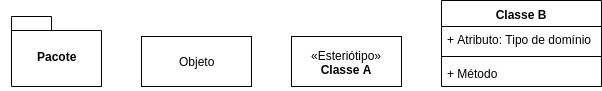
\includegraphics[width=1\hsize]{figuras/uml_obj.png}
  %\legend{Texto da legenda quando necessário.}
  \source{A autora}
\end{figure}

\textbf{Pacote}, em inglês \textit{package} é ``composto por um conjunto de elementos UML que podem ser de qualquer tipo, por exemplo, classes, associações e outras packages'' \cite[p.47]{queiroz2006tutorial}

\citeauthoronline{chonoles2011uml} definem \textbf{objeto} como ``qualquer item útil que tenha identidade, estrutura e comportamento'' \cite[p.46]{chonoles2011uml}, em outras palavras, identifica-se objeto como ``abstração que representa uma entidade do mundo real que pode ser algo concreto [...] ou abstrato'' \cite[p.]{tacla2007analise}.


Para \citeauthoronline{silva2007classesuml} ``\textbf{classe} descreve um conjunto de 
objetos com as mesmas propriedades (\textbf{atributo}), o mesmo comportamento (\textbf{métodos}), os mesmos relacionamentos com outros objetos e a mesma semântica'' \cite[p.11]{silva2007classesuml} corroborado por \citeonline[p.46]{chonoles2011uml} ao afirmar que classe é uma família de objetos. 

Segundo \citeonline[p.11]{silva2007classesuml}, o tipo de dado define o formato em que os dados devem ser armazenados dentro de um atributo, em outras palavras, ``o tipo de dado que descreve os tipos de valores que podem aparecer em cada coluna é presentado por um \textbf{domínio} de valores possíveis'' \cite[p.39]{navathe2011fundamentals}

``Os \textbf{esterótipos} significam um uso ou intenção especial e podem ser aplicados a quase qualquer elemento na notação da UML. Os estereótipos modificam o significado de um elemento e descrevem o papel desses elementos dentro do seu modelo'' \cite[p.16]{miles2006learning}

Como visto na figura \ref{uml_obj}, uma classe pode ser representada com mais de uma divisão, onde a primeira contém seu nome,  segunda seus atributos e a última seus métodos. De acordo com \citeonline[p.12]{silva2007classesuml}, a classe pode aparecer com três, duas ou até somente uma divisão, contudo caso só tenha uma divisão este deve conter as descrições da classe para respeitar as especificações da UML.

\begin{citacao}
    Uma das tarefas mais importantes quando se está modelando os dados de uma aplicação é a identificação de quais os relacionamentos que deverão ser mantidos no banco de dados, dentre os possíveis relacionamentos observáveis na realidade. [...] As cardinalidades associadas aos relacionamentos formam um conjunto de restrições de integridade que devem ser mantidas entre as instâncias dos objetos no banco de dados'' \cite[p.22]{lisboa2001modelagem}.
\end{citacao}

A cardinalidade é representada por uma notação de valores específica desenhada ao lado de fora da junção entre a conexão e uma classe. A tabela \ref{cardinalidade} apresenta alguns desses valores.
\begin{table}[!ht]{14cm}
  \caption{Cardinalidade.}\label{cardinalidade}
    \begin{tabular}{cc}
    \hline
    \rowcolor[HTML]{333333} 
    {\color[HTML]{FFFFFF} \textbf{Multiplicidade}} & {\color[HTML]{FFFFFF} \textbf{Significado}} \\ \hline
    \rowcolor[HTML]{EFEFEF} 
    \begin{tabular}[c]{@{}c@{}}0..1\end{tabular} & \begin{tabular}[c]{@{}c@{}} No mínimo zero (nenhum) e no máximo um. Indica que os objetos\\ das classes associadas não precisam obrigatoriamente estar\\ relacionados, mas se houver relacionamento indica que apenas uma \\ instância da classe se relaciona com as instâncias da outras classe \end{tabular} \\
    \begin{tabular}[c]{@{}c@{}}1..1 \end{tabular} & \begin{tabular}[c]{@{}c@{}} Um e somente um. Indica que apenas um objeto da classe se \\ relaciona com os objetos da outra classe\end{tabular} \\
    \rowcolor[HTML]{EFEFEF} 
    \begin{tabular}[c]{@{}c@{}}0..*\end{tabular} & \begin{tabular}[c]{@{}c@{}}No mínimo nenhum e no máximo muitos. Indica que pode ou não\\ haver instâncias da classe participando do relacionamento \end{tabular} \\
    \begin{tabular}[c]{@{}c@{}}*\end{tabular} & \begin{tabular}[c]{@{}c@{}} Muitos. Indica que muitos objetos da classe estão estão envolvidos\\ no relacionamento\end{tabular} \\
    \rowcolor[HTML]{EFEFEF} 
    \begin{tabular}[c]{@{}c@{}}1..*\end{tabular} & \begin{tabular}[c]{@{}c@{}}No mínimo um e no máximo muitos. Indica que há pelo menos um\\ objeto envolvido no relacionamento, podendo haver muitos\\ envolvidos\end{tabular} \\
    \begin{tabular}[c]{@{}c@{}}3..5\end{tabular} & \begin{tabular}[c]{@{}c@{}}No mínimo três e no máximo cinco. Indica que existem pelo menos\\ três instâncias envolvidas no relacionamento e que podem\\  ser quatro ou cinco as instâncias envolvidas, mas não \\ mais do que isso\end{tabular} \\ \hline
    \end{tabular}
  \source{\cite[p.13]{silva2007classesuml}}
\end{table}

Já os relacionamentos entre classes são desenhados como linhas que conectam essas classes. Cada tipo de relacionamento tem suas particularidades, logo são identificados e desenhados de formas diferentes. A figura \ref{uml_rela} ilustra os relacionamentos da UML e dá suas definições.

\begin{figure}[!ht]{15cm}
  \caption{Notações da UML B.} \label{uml_rela}
  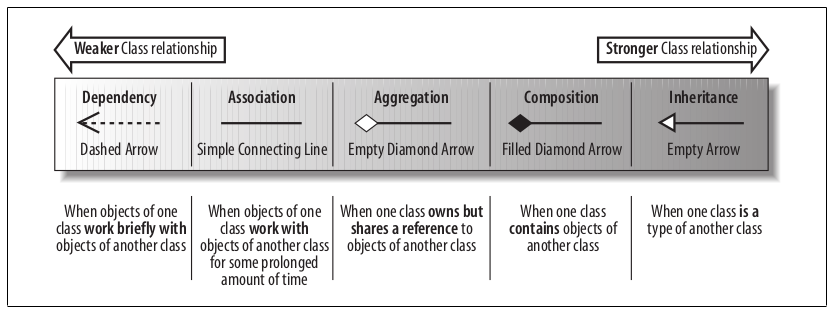
\includegraphics[width=1\hsize]{figuras/uml_relacao.png}
  %\legend{Texto da legenda quando necessário.}
  \source{\cite{miles2006learning}}
\end{figure}

Da figura \ref{uml_rela} tem-se que: `Dependência' ocorre quando objetos de uma classe possuem uma conexão breve com outra classe, `Associação' ocorre quando a conexão entre objetos de duas classes acontece durante um tempo prolongado, `Agregação' ocorre quando uma das classes está contida em outra sem depender da primeira para existir, `Composição' ocorre quando a classe contém objetos de outra classe e `Herança' ocorre quando uma classe é a especialização de outra classe, ou seja, é um tipo da outra classe.

Usando as notações apresentadas lê-se a figura \ref{uml_leitura} da seguinte forma:
a classe B, que é um geometria, agrega classe A, sendo que para cada tupla da classe A existe relacionada ao menos uma tupla da classe B.

\begin{figure}[!ht]{10cm}
  \caption{Ilustração para leitura na UML.} \label{uml_leitura}
  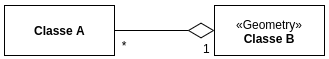
\includegraphics[width=0.75\hsize]{figuras/uml_leitura.png}
  %\legend{Texto da legenda quando necessário.}
  \source{A autora}
\end{figure}

\begin{citacao}
    A coleção de casos de uso representa todos os modos pelos quais o sistema pode ser utilizado pelos atores envolvidos. Um caso de uso é uma sequencia de \textbf{ações} realizadas colaborativamente pelos atores envolvidos e pelo sistema que produz um resultado significativo (com valor) para os atores. Um \textbf{ator} pode ser um usuário ou outro sistema. \cite[p.10]{tacla2007analise}
\end{citacao}


``Especialização de atores representa que um conjunto deles possui responsabilidades ou características em comum '' \cite[p.29]{tacla2007analise}. É importante ressaltar que herança entre atores, generalização e especialização entre atores se refere ao mesmo tipo de relacionamento. Assim, observando a figura \ref{uml_casouso}, identifica-se os atores (a) e (b). O ator (b) é capaz de realizar a ação I, enquanto o ator (a) é capaz de realizar a ação II. Na generalização (c) do ator (b) para o ator (a) tem-se que (b) pode realizar os mesmos casos de uso que (a), o que significa que o ator (b) pode realizar a ação I e a ação II. 

\begin{figure}[!ht]{10cm}
  \caption{Notações da UML C.} \label{uml_casouso}
  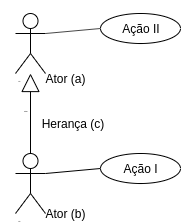
\includegraphics[width=0.5\hsize]{figuras/uml_casosuso.png}
  %\legend{Texto da legenda quando necessário.}
  \source{A autora}
\end{figure}

De acordo com \citeonline[p.10]{tacla2007analise} o diagrama de casos de uso fornece um panorama visual das funcionalidades do sistema, isso significa que uma descrição textual, ou seja um documento de texto é gerado para detalhar os casos de uso.

%falar da relacional(?)
Outra forma de modelar dados, como discutido previamente, é pelo modelo relacional. Enquanto o mesmo não é ideal para modelagem de dados geográficos, como discutido nos últimos itens, devido a uma questão de acessibilidade à ferramenta de implementação em certo momento foi gerado um modelo relacional, logo algumas particularidades não apresentadas até o momento serão descritas a seguir.

\subsubsection{Modelo Entidade-Relacionamento}
``O modelo entidade-relacionamento adota uma
visão natural onde o mundo real consiste em entidades e relacionamentos'' \cite[p.1]{codd1970relational}

\citeauthoronline{heuser1998projeto} afirma que \textbf{entidade} é ``conjunto de objetos da realidade modelada sobre os quais deseja-se manter informações no banco de dados'' \cite[p.23]{heuser1998projeto}, enquanto \textbf{relacionamento} é definido como ``conjunto de associações entre entidades'' \cite[p.24]{heuser1998projeto}. Observando  figura\ref{relacional_a} tem-se que no diagrama 1, A e C são entidades enquanto B é um relacionamento.

\begin{figure}[!ht]{10cm}
  \caption{Ilustração de um diagrama entidade-relacionamento.} \label{relacional_a}
  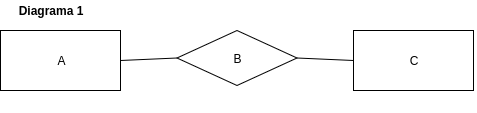
\includegraphics[width=0.75\hsize]{figuras/relacional_a.png}
  %\legend{Texto da legenda quando necessário.}
  \source{A autora}
\end{figure}

Outras duas definições importantes são as de \textbf{chave estrangeira} e \textbf{chave primária}.
\citeonline[p.380]{codd1970relational} define como chave primária (PK - Primary key) uma coluna (ou combinação de colunas) em que seus elementos jamais se repetem. Uma entidade sempre deve possuir ao menos uma PK e a mesma nunca deve ter um elemento nulo. O mesmo autor também define chave estrangeira (FK - Foreign Key) como elementos de uma relação que referenciam outros elementos da mesma relação ou elementos de uma relação diferente. A definição destas chaves é importante viabilizar a integridade de referência, que por sua vez é mecanismo com o qual registramos as relações entre as instâncias do banco de dados.

\begin{figure}[!ht]{10cm}
  \caption{Exemplo de indicação de FK e PK em tabelas.} \label{fk_pk}
  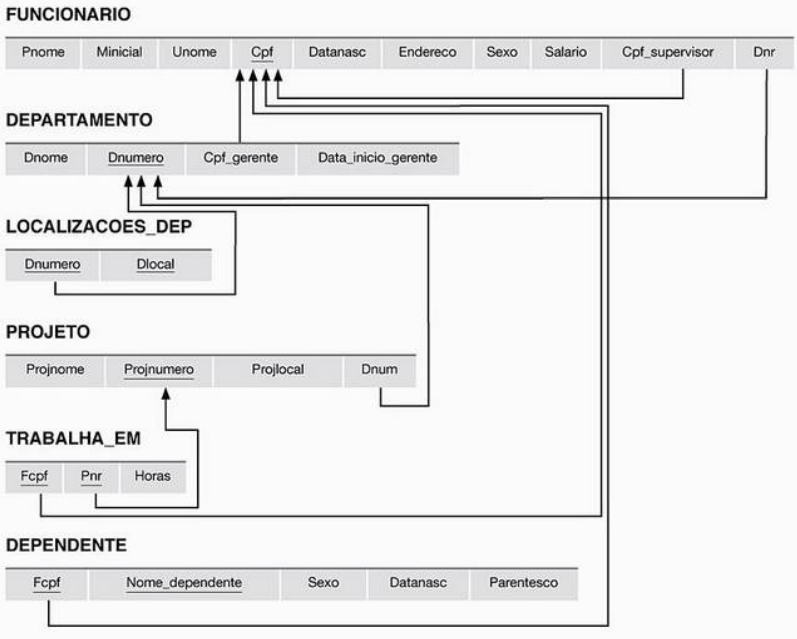
\includegraphics[width=1\hsize]{figuras/fk_pk.png}
  %\legend{Texto da legenda quando necessário.}
  \source{\cite{navathe2011fundamentals}}
\end{figure}
Na figura \ref{fk_pk}, as chaves primárias tem seus nomes sublinhados enquanto as chaves estrangeiras são indicadas pelo uso de `setas', assim o atributo do qual a seta sai se referencia ao atributo à que a seta indica.


\citeonline[p.45-49]{navathe2011fundamentals} usa o termo `relação' para descrever a tabela, logo, relação pode ser tanto entidade quanto relacionamento. Porém um diagrama entidade-relacional pode ser representado de formas diferentes. ``O usuário [...] pode seguir uma disciplina que toda entidade ou relacionamento deve ser mapeado em um registro [...] tudo que você precisa fazer é trocar os diamantes para caixas e para adicionar pontas de seta nas linhas apropriadas'' \cite[p.32]{chen1976entity}. Assim:

\begin{figure}[!ht]{10cm}
  \caption{Ilustração de um diagrama relacional.} \label{relacional_b}
  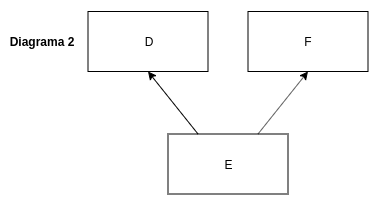
\includegraphics[width=0.5\hsize]{figuras/relacional_b.png}
  %\legend{Texto da legenda quando necessário.}
  \source{A autora}
\end{figure}

No diagrama 2 da figura \ref{relacional_b} sem tem uma dificuldade maior de distinguir relacionamento de entidade porém percebe-se que E possui um chave estrangeira referenciada a D e uma chave estrangeira referenciada a F. É importante mencionar que ``setas no diagrama da estrutura de dados nem sempre representam relações de entidades'' \cite[p.31]{chen1976entity}.

Deve ser lembrado que das linguagens de modelagem apresentadas, somente as partes relevantes para o trabalho foram apresentadas. Suas notações se estendem a mais do que o visto até o presente momento.

\section{Normas}
Existem normas nacionais e internacionais que padronizam como os dados e metadados de tipos específicos devem ser modelados e implementados. Durante a construção do projeto piloto, visando a padronização apresentada nesses documentos, foi realizada uma pesquisa sobre normas, tanto nacionais quanto internacionais, que pudessem ser utilizadas neste trabalho. 

Dentre as normas nacionais existe o \textit{Perfil de Metadados Geoespaciais do Brasil - PMGB}. 
Segundo \citeonline[p.86]{inde2010} devido à tendência mundial na época da definição de perfis de metadados geográficos baseados na ISO:19115:2003, a CONCAR (Comissão Nacional de Cartografia) especificou e consolidou o PMGB através do CEMG (Comitê de Estruturação de Metadados Geoespaciais). ``Trata-se de uma iniciativa para ordenar a geração, armazenamento, acesso, compartilhamento, divulgação e uso dos dados geoespaciais - aqueles que se distinguem pela componente espacial, que associa cada entidade ou fenômeno a uma localização na Terra '' \cite[p.10]{pmgb2009}

``A proposta do Perfil MGB inclui a maioria das seções de metadados presentes na norma ISO 19115'' \citeonline[p.86]{inde2010}. Dentre eles os mais relevantes para o trabalho são \textbf{MD\_SpatialRepresantation}, relativos as informações de representação espacial e \textbf{MD\_ReferenceSystem}, responsável por descrever o sistema de referencia utilizado.  

Já no âmbito internacional, para dados geoespaciais, a organização de padronização mais importante é o \textit{Open Geospacial Consortium - OGC}. 
\begin{citacao}
O Open Geospatial Consortium (OGC) é um consórcio internacional de mais de 530 empresas, agências governamentais, organizações de pesquisa e universidades orientadas a tornar informações e serviços geoespaciais (localização) FAIR -Findable, Accessible, Interoperable, and Reusable (Localizáveis, Acessíveis, Interoperáveis e Reutilizáveis). \cite[p.1]{ogc}
\end{citacao}

``Os produto do trabalho do OGC são apresentados sob forma de especificações de interfaces e padrões de intercâmbio de dados'' \cite[p.66]{queiroz2006tutorial}.

Porém tanto o PMGB, quanto a documentação da OGC baseia-se nos documentos produzidos pela \textit{International Organization for Standardization - ISO's}.

\begin{citacao}
    A ISO é uma organização internacional não governamental independente, com 164 membros de organismos nacionais de padrões. Por meio de seus membros, reúne especialistas para compartilhar conhecimento e desenvolver Normas Internacionais voluntárias, baseadas em consenso e relevantes para o mercado, que apoiam a inovação e fornecem soluções para os desafios globais. [...] A ISO publicou 22873 Normas Internacionais e documentos relacionados, cobrindo quase todos os setores, desde tecnologia, segurança alimentar, agricultura e saúde.\cite[p.1]{iso}
\end{citacao}


A ISO / TC 211 é um comitê técnico, responsável pela elaboração de ISO's relacionadas as informações geográficas digitais. Seu trabalho esta intimamente ligado à produção da documentação gerada pela OGC.

Dentre as ISO's elaboradas pela ISO/TC 211  disponíveis, algumas das que foram pesquisadas, de acordo com \citeauthoronline{isomodels}, são:
\begin{itemize}
    \item ISO 6709 Standard representation of geographic point location by coordinates - Trata da representação de latitude, longitude e altitude de pontos geográficos.
    \item ISO 19115 Metadata - Trata de metadados relacionados direta ou indiretamente a dados geográficos.
    \item ISO 19123 Schema for coverage geometry and functions - Define um modelo abstrato de coberturas geográficas.
    \item ISO 19129 Imagery, gridded and coverage data - Gera uma estrutura aplicada para software que tratam de dados relacionados ao sensoriamento remoto, a fotogrametria e ao processamento de imagem, como imagens, coberturas etc.
    \item ISO 19130 Imagery sensor models for geopositioning - Trata de dados e metadados de sensores com o objetivo de fornecer uma interoperabilidade para dados de imagens.
    \item ISO 19136 Geography Markup Language (GML) - Trata da codificação do xml voltado para informações geográficas.
    \item ISO 19159 Calibration and validation of remote sensing imagery sensors and data - Trata dos padrões necessários para a validação e calibração de sensores imageadores aéreos e orbitais.
\end{itemize}

A partir dessa pesquisa percebeu-se uma ausência de normas nacionais voltadas exclusivamente para os dados fotogramétricos. Durante a mesma ocorreu uma dificuldade no acesso aos documentos por inteiro das ISO's, acarretando no acesso limitado aos dados públicos ou parciais desses documentos. Deste acesso percebeu-se não haver uma ISO que trata-se exclusivamente de dados voltados para a fotogrametria. Baseado nessas experiências julgou-se não haver normas estabelecidas e acessíveis, tanto em âmbito nacional quanto internacional, que atendessem às necessidades deste trabalho. Assim, foi decidido pela modelagem independente dos dados fotogramétricos, como demonstrado na metodologia apresentada no capítulo \ref{met}, tomando por base principalmente os modelos pré-existentes de trabalhos anteriores no projeto E-foto. 


%=====================================================================
\chapter{Metodologia} \label{met}
%=====================================================================

O projeto piloto, resultante do modelo de dados proposto, deve ser capaz de suportar a carga de parte do acervo de dados do LFSR do Departamento de Engenharia Cartográfica da Universidade Estadual do Rio de Janeiro - UERJ. Para a modelagem do banco foi necessária a identificação e organização dos dados de um projeto fotogramétrico em meio digital. O modelo do banco engloba grande parte do processo aerofotogramétrico, deixando em aberto possibilidades para futuras expansões que venham a incluir outros processos de sensoriamento remoto que não sejam realizados pela fotogrametria aérea tradicional.

A metodologia adotada caracteriza-se pelas seguintes atividades principais: o levantamento de requisitos, a criação de um modelo conceitual, a implementação do banco de dados piloto, a carga de dados e execução de de testes por intermédio de consultas, visões e funções de recuperação da informação. O levantamento de requisitos envolve a identificação das necessidades e foi feito por meio de várias reuniões, explicadas em maiores detalhes no item \ref{conceitos_requisitos}, entre integrantes da equipe técnica do LFSR e a autora do trabalho. Até a conclusão da primeiro modelo, como resultado da atividade de modelagem o processo de desenvolvimento adotado foi baseado no modelo monolítico. Em determinado momento, observado a possibilidade do não cumprimento dos prazos estabelecidos, o processo monolítico foi descartado e as informações até então geradas foram incorporadas num novo processo, o processo ágil (para mais informações nesses processos ver item \ref{proc}). Por último, uma implementação de banco de dados piloto foi efetuada a partir das versões geradas do modelo no ciclo de desenvolvimento ágil. Cada atualização modelo passou a ser refletida imediatamente no piloto, sobre o qual eram efetuadas cargas de dados e testes como meio de verificação e validação do modelo.



\section{Levantamento e Análise de Requisitos}

Pensando em como solucionar o problema real, que é o armazenamento e organização de dados de seu acervo, foram feitas uma série de perguntas que levaram a idealização das necessidades do LFSR e a realização deste trabalho. É importante comentar que todos os questionamentos e respostas encontrados foram realizados durante as reuniões, seguindo a técnica de \textit{brainstorming}, entre a autora e integrantes da equipe técnica do LFSR.


\subsection{Diagrama de Caso de Uso}

Duas perguntas iniciais tratadas em \textit{brainstorm} foram: \textit{``qual é o perfil do usuário atuante no laboratório?''} e \textit{``quais devem ser suas ações e atuações dentro do banco de dados do laboratório?''}. Para responder tais perguntas foi elaborado um diagrama de caso de uso.

O diagrama de caso de uso, como explicado no item\ref{uml2.0}, é um diagrama que modela os casos de uso, ou seja, as ações e restrições de um ator no banco de dados. Este diagrama viabiliza a captura dos requisitos de sistema na forma estruturada. Devido ao grande volume de requisitos a serem tratados no escopo projeto, este foi o único detalhado sobre a forma de diagrama. Sugere-se que trabalhos futuros da equipe técnica do LFSR tratem da estruturação dos demais requisitos.

Foram estabelecidos durante o levantamento 4 níveis de atuação para usuários. O `nível 0' corresponde ao \textbf{administrador}, o `nível 1' corresponde ao \textbf{professor}, o `nível 2' corresponde ao \textbf{aluno} e o `nível 3' corresponde ao \textbf{visitante} anônimo.

A figura \ref{usecase} apresenta as ações (funções permitidas) de cada usuários no banco. Percebe-se que quanto maior o nível do usuário, maiores são as restrições sobre o mesmo de uso aplicadas. O anônimo consegue ler qualquer dado que seja público do banco de dados. No nível acima, o aluno é capaz de criar, editar e deletar um projeto, além de realizar leitura dos dados públicos como fariam os usuários anônimos e dos dados de seus próprios projetos. A edição e extinção de um projeto só pode ser realizada se o projeto for do usuário aluno. O usuário professor, por sua vez é capaz de realizar todas as ações do usuário aluno. Sendo também capaz criar alunos e associá-los a grupos (turmas). Por fim, no nível mais especializado, encontra-se o administrador. Este realiza todas as funções dos outros usuários e estende as capacidades dadas ao professor para criação de usuários do tipo professor. Deletar e alterar qualquer usuário (e seus níveis) no banco são atribuições delegadas ao administrador. Idealmente, recomenda-se que o administrador seja o DBA (\textit{Database Administrator}) do banco de dados proposto.

\begin{figure}[!H]{16cm}
  \caption{Diagrama de caso de uso} \label{usecase}
  \centering
  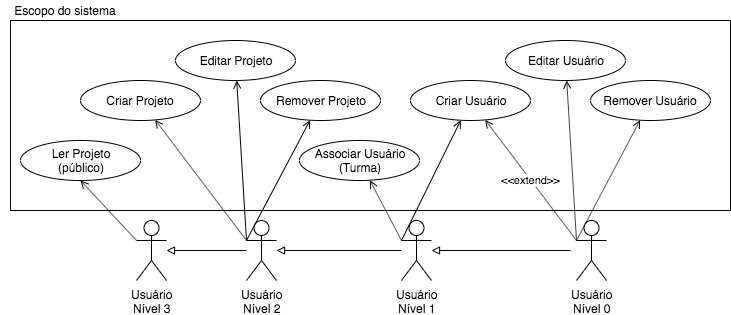
\includegraphics[width=1.0\hsize]{figuras/diag_use_case.png}
  \legend{Nível 0: Administrador; Nível 1: Professor; Nível 2: Aluno; Nível 3: Visitante (Anônimo).}
  \source{A autora, 2018.}
\end{figure}

O digrama tem como função mapear as interações previstas dos atores do LFSR com o banco de dados. A documentação gerada pelo mesmo se encontra no apêndice \ref{ap2}. Como as restrições a serem aplicadas dependem de comandos SQL do tipo DCL(\textit{Data Control Language}), o código de implementação do projeto piloto não incluíram os requisitos modelados neste diagrama de caso de uso. Isto significa que este requisito foi levantado, mapeado, porém não implementado.

Da análise imediata dos requisitos são identificadas duas entidades sobre as quais irão operar as funcionalidades registradas como requisitos. São o ``usuário do LFSR'' e o ``projeto fotogramétrico''. Por simplificação, as seções seguintes irão adotar convenções como, por exemplo, ``requisitos de projeto'' para referir-se às funções de inserção, recuperação, atualização e, em alguns casos, remoção, da entidade ``projeto'' fotogramétrico, ou seja, neste trabalho está sendo simplificado ``requisitos de pertinência do projeto fotogramétrico'' para a primeira forma apresentada. Demais requisitos de associação das entidades ou imposição de regras serão nomeados diretamente, sem simplificação, quando necessário.


\subsection{Identificação das Entidades Principais do Acervo} \label{entidades}

Logo de início, foi questionado \textit{``quais dados comporiam o acervo?''}. A resposta levou à identificação dos tipos de dados encontrados no acervo, compostos em sua grande maioria, por imagens em formato analógico (fotogramas). Foram encontrados, também, alguns registros de projetos de alunos antigos ou projetos disponibilizados ao LFSR, registros de pontos e dados relacionados a sensores, não necessariamente vinculados aos projetos fotogramétricos.

O software e-foto, como parte fundamental do LFSR, tem capacidade de trabalhar com outros projetos fotogramétricos fora os disponibilizados atualmente em seu \textit{website}. O próprio laboratório possui total capacidade de trabalhar com outros projetos, sejam eles fotogramétricos ou de sensoriamento remoto. Isso leva ao segundo questionamento \textit{``de que formas esse dados poderiam ser expandidos?''}. Para o qual registra-se no contexto deste trabalho que atualmente, o conjunto de dados não é mais composto só pela realidade atual do acervo do LFSR, mas também de uma previsão da realidade futura. Dessa forma, ao responder tal questionamento foi possível prever, em parte, a criação de uma solução que, em pouco tempo, poderia se tornar obsoleta. Nesta hipótese, o conjunto de dados previsto engloba o acervo e os dados relacionados a um projeto aerofotogramétrico tradicional e estima-se a necessidade de extensão contínua do modelo, enquanto houverem evoluções do conjunto de dados do acervo.

Os requisitos principais e por consequência a entidade principal é identificada quando o objetivo da fotogrametria é definido como ``a reconstrução de um espaço tridimensional, chamado de espaço-objeto, a partir de um conjunto \textbf{não vazio de imagens bidimensionais}, chamado de espaço-imagem'' \cite[p.16]{coelho2007fotogrametria}. Assim fica claro que a entidade fundamental dentre aquelas que mapeiam o acervo para o laboratório de fotogrametria é a \textbf{imagem}. 

Para auxiliar a identificação de outras entidades principais fez-se uso do fluxo de trabalho do projeto E-Foto. A partir dele foram destacadas as atividades da fase de Inicialização do Projeto, descrito na seção \ref{efoto}, que apresenta o fluxo de trabalho fotogramétrico. Os dados de \textbf{projeto}, como \textbf{voo} e \textbf{sensor}, são atribuídos na atividade de Criação e Gerenciamento do Projeto Fotogramétrico. Na atividade seguinte, Aquisição e Cadastro de Dados são fornecidos informações a respeito das \textbf{imagem} e dos \textbf{pontos}, adquiridos nos levantamentos aéreo e terrestre, respectivamente. Orientação Interior e Orientação Exterior são atividades de processamento, e, enquanto importantes, ambas geram parâmetros relacionados à imagem e, por tanto, caracterizam a presença de entidades fracas. Por último, as fases de Geração de produtos e Integração, que envolvem o processamento e distribuição dos \textbf{produtos} finais da fotogrametria, ficaram fora do escopo deste trabalho. A relação entre as entidades principais identificadas podem ser ilustrados como na figura \ref{requisitos}.

\begin{figure}[!ht]{13cm}
  \caption{Identificação das entidades principais pela análise de requisitos} \label{requisitos}
  \centering
  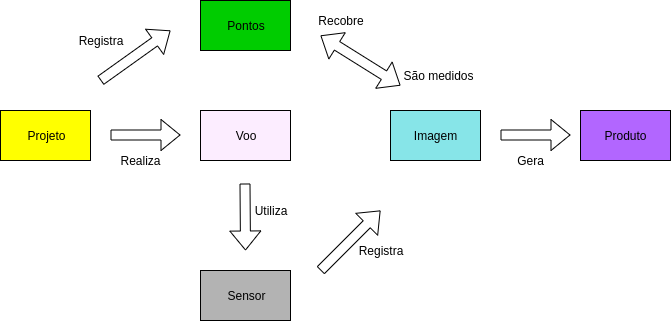
\includegraphics[width=1.0\hsize]{figuras/diagrama_requisitos.png}
  %\legend{Texto da legenda quando necessário.}
  \source{A autora, 2018.}
\end{figure}

Todo o projeto fotogramétrico, como comentado no item \ref{efoto}, é responsável pelo armazenamento de metadados relativos ao processo fotogramétrico. É nele que dados como: responsável pelo projeto; criação e data de modificação etc, são armazenados. 
Voltando aos itens \ref{sensor_img} e \ref{foto_trad}, para todo levantamento aéreo, com finalidade fotogramétrica, é indispensável a presença do sensor imageador na aeronave, pois o mesmo é responsável pela aquisição das imagens.
Segundo \citeonline[p.32-39]{projeto1999dalmolin} pontos de controle ou apoio devem ser demarcados na região fotografada, podendo ser medidos antes do levantamento aéreo ou depois. Os projetos fotogramétricos podem depender ainda de pontos fotogramétricos, cujas coordenadas no espaço objeto só serão determinadas ao final da fase de inicialização fotogramétrica. Porém, o autor deixa claro que os pontos, independentemente do tipo ou finalidade, devem ser visíveis nas fotografias, de modo a serem utilizados no projeto.
Por fim, percebe-se na obra de \citeonline{coelho2007fotogrametria}, que diversos produtos são gerados a partir do processo fotogramétrico. Sabendo que, nesses processos, a imagem pode ser considerada como dado central, fica fácil perceber que o produto fotogramétrico é gerado, independentemente do método, a partir das imagens cadastradas.

Assumindo que esses são os principais requisitos de persistência e estão associados à entidades fortes, foi adotado que para cada entidade principal existe um pacote de mesmo nome. Cada pacote deve receber o nome de suas respectivas entidades principais e conter demais entidades diretamente relacionadas às principais.

Nesse momento, o próximo passo foi questionar: \textit{``exitem normas que identifiquem e padronizem essas entidades?''}, \textit{``caso essas normas existam, elas atendem os objetivos estabelecidos neste trabalho?''}. Tentando responder a essas perguntas, chegou-se ao Perfil de Metadados Geográficos do Brasil \cite{pmgb2009}. Porém o mesmo, como o próprio nome diz, trata de metadados e inclui imagem como tal, entrando em conflito com a expectativa da fotogrametria, que considera a imagem seu dado principal.

A questão anterior foi também analisada no âmbito internacional. À primeira vista, a padronização esperada foi pesquisada na documentação da OGC, mas como estava baseada nas normas de padronização ISO o que implicou na necessidade de se consultar as mesmas. Neste momento foram encontrados muitos obstáculos. Como, por exemplo, o custo de aquisição da ISO, que limita o acesso às mesmas, restringindo à parte da documentação disponível ao acesso público. Dentre as ISO pesquisadas foi constatado que enquanto algumas atendiam parte das entidades esperadas para alguns pacotes, todas se desdobravam em outras ISO, ao ponto em que a documentação necessária pra a criação do modelo seria demasiadamente extensa. Assim, ao se tentar utilizar todas as ISO, necessárias para criação de parte do modelo, se acabaria por ter um novo padrão, o que foge ao objetivo inicial.

Ao considerar todos esses fatores, observou-se que não foi encontrado uma norma, ou conjunto de normas que atendesse o projeto. Assim, partiu-se para a identificação das outras entidades envolvidas em um processo fotogramétrico com a seguinte pergunta \textit{``quais entidades complementam as já identificadas e como elas se comunicam?''}. No item \ref{model} é descrito como foi realizada a modelagem da comunicação entre as entidades. Porém, antes desse modelo ser criado, deve-se responder a primeira parte dessa pergunta e identificar os requisitos faltantes para complementar um processo fotogramétrico.  

\citeonline[p.1-6]{projeto1999dalmolin} define três fases a serem realizadas durante o planejamento de projeto fotogramétrico com fotografias aéreas. As duas primeiras fases resumem, em poucas palavras, boa parte das entidades e onde elas se encontram no processo fotogramétrico:

 \begin{itemize}
     \item Planejamento de voo leva em consideração as informações relativas ao terreno. As informações do sensor, usadas junto com os dados do terreno, permitem ao técnico definir linhas de voo, porcentagem de sobreposição entre as fotografias tomadas, quantidade final de fotografias tomadas, direção de voo etc.
     \item Planejamento do controle de terreno e execução dos levantamentos de campo. Estes geram os pontos que são medidas nas imagens.
 \end{itemize}

Analisando o planejamento de voo, identifica-se a existências de dados relativos ao \textbf{voo}, ao \textbf{terreno}, ao \textbf{sensor}, ao rodapé da imagem, que nada mais é do que à projeção, no terreno, das fotografias tomadas sobre o terreno e as próprias \textbf{imagens}. O sensor, por sua vez, define a \textbf{geometria} da fotografia tirada, sendo o \textit{frame} (quadro) o caso mais comum. Na segunda fase são identificados os \textbf{pontos}, que podem ser obtidos através do \textbf{levantamento} topográfico. Esses pontos formam \textbf{coleções} associadas pelo levantamento à região geográfica em que se encontram.

\citeonline[p.89]{coelho2007fotogrametria} comentam que para que sejam possíveis as medições de coordenadas no espaço-imagem, as imagens do voo acabam por ser `orientadas'. Ou seja, os parâmetros das orientações interior e exterior devem ser incorporados às imagens durante o processo fotogramétrico. O processo de fototriangulação é o principal meio de computação dos parâmetros de orientação, contudo processos para imagens isoladas podem ser executados como alternativa, a exemplo do processo de ressecção espacial. Este fato em junção da previsão do modelo poder abranger outros processos levam à caracterização dos \textbf{parâmetros} como entidades agregadas (entidades fracas), que se relacionam às imagens e a um modelo paramétrico adotado no projeto, para descrever o sistema de equações adotadas no projeto. Estima-se que tais indicações podem auxiliar na fixação do modelo para futuras entradas de dados de outros processos como ocorreria na implementação do uso de imagens provenientes de satélite que geralmente são acompanhadas de RPCs.

Vale ressaltar que nem todos o requisitos de persistência identificados geraram entidades fortes no modelo conceitual. Consequentemente algumas entidades vão surgir durante a especificação do modelo que antecede a implementação. Por exemplo, a representação de \textbf{rodapé} necessita de um maior detalhamento para que sua entidade possa ter uma especificação como classe e a devida associada com a entidade imagem mapeada. Rodapé da imagem, como visto na figura \ref{foot}, refere-se à região de cobertura no terreno associada à respectiva imagem. Isso significa que nem todo termo fotogramétrico está elicitado nos requisitos levantados para as primeiras versões do modelo e torna evidente a necessidade de um modelo de desenvolvimento ágil. Por fim, a adição deste requisito, implica na possibilidade de adição de diversas entidades no modelo como faixa e par que não eram bem estruturados até a integração do conceito de rodapé.

\begin{figure}[!ht]{10cm}
  \caption{Exemplo de rodapé de imagens.} \label{foot}
  \centering
  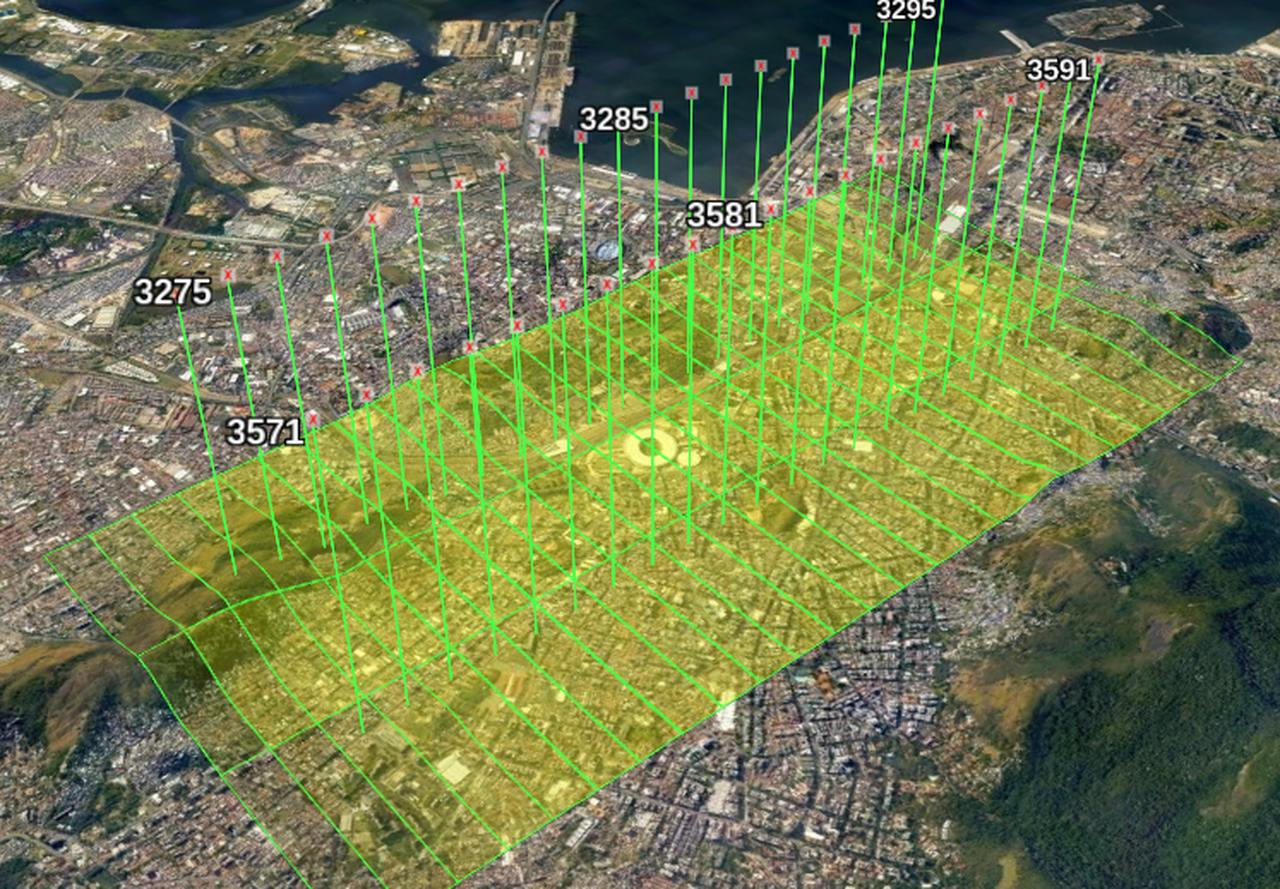
\includegraphics[width=1\hsize]{figuras/footprint.jpg}
  \legend{Imagem adaptada pela autora no software Google Earth Pro, utilizando os dados de levantamento aéreo sobre o Rio de Janeiro no de 2003 realizado pelo IPP}
  \source{A autora, 2019.}
\end{figure}

Como comentado no item \ref{foto_trad}, existe uma sobreposição de imagens acarretando em, no mínimo, a existência de um ``par de imagens''. Esse par de imagens são necessários para ocorrer a estereoscopia. Várias imagens tomadas em sequência formam uma ``faixa''. O grupo de faixas de um mesmo voo podem formar um ``bloco''.

As entidades destacadas até então podem ser subdivididas em três categorias: (1) entidades principais; (2) entidades complementares; e (3) entidades derivadas. Entidades complementares são entidades internas aos pacote para completude ou associatividade do modelo, tendo como dados de entrada, dados brutos ou dados de associação dos elementos presentes no acervo ao projeto fotogramétrico. Já as entidades de dados derivados armazenam dados obtidos através de cálculos. A tabela \ref{entidades_cat} mostra um exemplo de distribuição das entidades analisadas em suas respectivas categorias.

\begin{table}[!ht]{14cm}
  \caption{Exemplos de entidades separadas por categorias.}\label{entidades_cat}
    \begin{tabular}{ccc}
    \hline
    \rowcolor[HTML]{333333} 
    {\color[HTML]{FFFFFF} \textbf{Principal}} & {\color[HTML]{FFFFFF} \textbf{Complementar}} & {\color[HTML]{FFFFFF} \textbf{Derivadas}} \\ \hline
    \rowcolor[HTML]{EFEFEF} 
    \begin{tabular}[c]{@{}c@{}}Projeto\end{tabular} & \begin{tabular}[c]{@{}c@{}}Terreno\end{tabular} & \begin{tabular}[c]{@{}c@{}}Parâmetros\end{tabular} \\
    
    \begin{tabular}[c]{@{}c@{}}Ponto\end{tabular} & \begin{tabular}[c]{@{}c@{}}Levantamento do terreno\end{tabular} & \begin{tabular}[c]{@{}c@{}}\textit{Rodapé}\end{tabular} \\
    
    \rowcolor[HTML]{EFEFEF} 
    \begin{tabular}[c]{@{}c@{}}Sensor\end{tabular} & \begin{tabular}[c]{@{}c@{}}Especificações do sensor\end{tabular} & \begin{tabular}[c]{@{}c@{}}Produtos\end{tabular} \\
    
    \begin{tabular}[c]{@{}c@{}}Voo\end{tabular} & \begin{tabular}[c]{@{}c@{}}Bloco\end{tabular} & \begin{tabular}[c]{@{}c@{}}\end{tabular} \\
    
    \rowcolor[HTML]{EFEFEF} 
    \begin{tabular}[c]{@{}c@{}}Imagem\end{tabular} & \begin{tabular}[c]{@{}c@{}}Faixa\end{tabular} & \begin{tabular}[c]{@{}c@{}} \end{tabular} \\
    
    \begin{tabular}[c]{@{}c@{}}\end{tabular} & \begin{tabular}[c]{@{}c@{}}Par\end{tabular} & \begin{tabular}[c]{@{}c@{}}\end{tabular} \\ 
    %\rowcolor[HTML]{EFEFEF} 
    %\begin{tabular}[c]{@{}c@{}}\end{tabular} & %\begin{tabular}[c]{@{}c@{}}\end{tabular} &
    %\begin{tabular}[c]{@{}c@{}}\end{tabular} \\
    \hline
    \end{tabular}
  \source{A autora, 2019}
\end{table}



\section{Modelagem}\label{model}

Após o levantamento e análise de requisitos, o passo seguinte foi de modelagem. Este consistiu na construção de diagramas para especificar as classes que permitissem a representação das entidades a serem persistidas no banco, levando em consideração suas conexões e possíveis agrupamentos em pacotes. Como explicado no item \ref{mod_bd}, a modelagem adotada deve suportar dados alfanuméricos e geográficos. A linguagem escolhida foi a UML 2.0 e a especificação de classes e tipos de dados está inclusa nos apêndices deste trabalho. A seguir, serão apresentadas as justificativas e tomadas de decisão que levaram ao conjunto de classes modeladas, com dicionários de dados para estas classes e os diagramas de pacotes.


\subsection{Modelo Orientado a Objetos}

O modelo idealizado para o LFSR tem sua nomenclatura escrita em inglês. Essa decisão foi tomada em função da internacionalização do projeto E-Foto. Como este, por sua vez, serviu de base para muitas partes do modelo desenvolvido neste trabalho, optou-se por seguir este padrão para nomenclatura. O que torna o modelo em construção aderente aos trabalhos anteriores que foram desenvolvidos no projeto E-Foto. Para o modelo ser elaborado foi necessário conhecer todos os detalhes de um projeto fotogramétrico. O conhecimento se baseia na leitura de diferentes autores e obras, todos presentes na bibliografia deste trabalho.

Muitos autores começam explicando o mapeamento fotogramétrico pelo plano de voo, indicando que o planejamento deve ser a primeira atividade a ser feita. Enquanto essa concepção não está errada, ao se planejar um voo o projeto fotogramétrico é iniciado. Por se tratar da modelagem de um banco de dados, deve-se considerar os metadados do mapeamento fotogramétrico. Isso significa que o primeiro objeto a ser modelado é a classe \textit{Project}:

\begin{description}[labelwidth=2cm, itemsep=-0.3cm]
    \item [Classe Project]
    \item [Id:] Índice numérico;
    \item [Name:] Nome do projeto;
    \item [Owner:] Responsável, ou dono, do projeto;
    \item [Date\_add:] Data de criação do projeto no banco;
    \item [Date\_mod:] Última data de modificação do projeto;
    \item [Software:] Programa computacional responsável pelo processamento de dados;
    \item [Id\_srs:] Referência para a classe \textit{Srs}.
\end{description}

A figura \ref{project}, no apêndice \ref{ap0}, resume os atributos da classe \textit{Project} e os tipos de dados adotados durante sua implementação.

Qualquer projeto armazenado no banco, por conter a dados geográficos, deve possuir projeção cartográfica, sistema de referência geodésico e quaisquer dados complementares destes primeiros. É importante saber quais são os referenciais e projeções aplicáveis para proceder transformações de compatibilização nos dados de entrada e saída para cada projeto. A classe \textit{Srs} é responsável por armazenar esses dados:

\begin{description}[labelwidth=2cm, itemsep=-0.3cm]
\item [Classe Srs]
\item [Id:] Índice numérico;
\item [Epsg:] Referência ao  campo `srid' na tabela `spatial\_ref\_sys', comum nos SGBDs espaciais.
\end{description}

O EPSG é um vantagem presente em algumas extensões de bancos de dados espaciais. O Grupo de Pesquisa Petrolífera Européia ( \textit{European Petroleum Survey Group} - EPSG) é responsável pela criação dos `Códigos EPSG'. Informalmente conhecidos como simplesmente EPSG, essa lista de valores numéricos é uma combinação que serve de índice para sistemas de referência de coordenadas em todo o planeta.

As coordenadas do ponto central da região geográfica de trabalho, também são associadas a um projeto fotogramétrico. Tal dado se justifica em função da correção do efeito sistemático da curvatura da Terra no cálculo da aerotriangulação, onde é utilizado o método de ajustamentos de um bloco de imagens por feixes perspectivos. Esse efeito é notável em escalas médias e pequenas, isto é, menores ou iguais à 1:30.000, sendo geralmente negligenciado para escalas cadastrais (1:10.000 e maiores). A classe \textit{Cg\_central\_area} inclui tais informações.

\begin{description}[labelwidth=2cm, itemsep=-0.3cm]
\item [Classe Cg\_central\_area]
\item[Id\_proj:] Referência para a classe \textit{Project};
\item[Proj\_ctr:] Coordenadas planimétricas do centro da região de interesse do projeto.
\end{description}

Estas três classes compõem o pacote \textbf{Project}. A figura \ref{pack_proj} ilustra como essas classes se comunicam entre si, e com outros pacotes.

\begin{figure}[!ht]{13cm}
  \caption{Pacote Project} \label{pack_proj}
  \centering
  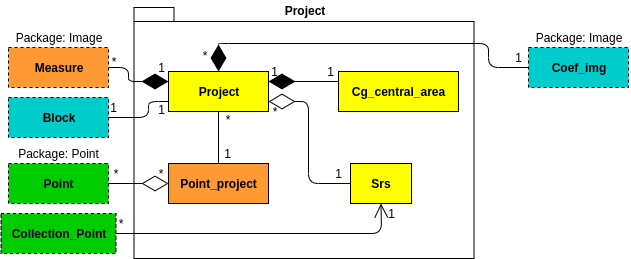
\includegraphics[width=1\hsize]{figuras/package_proj.png}
  %\legend{Texto da legenda quando necessário.}
  \source{A autora, 2019.}
\end{figure}

Definido o projeto pode-se partir para o levantamento aéreo. No planejamento de voo, dados do terreno da região a ser sobrevoada são coletados. Estes devem ser armazenados na classe \textit{Terrain}.

\begin{description}[labelwidth=2cm, itemsep=-0.3cm]
\item [Classe Terrain]
\item[Id:] Índice numérico;
\item[Alt\_max:] Valor da altitude máxima do terreno em metros;
\item[Alt\_min:] Valor da altitude mínima do terreno em metros;
\item[Alt\_med:] Valor da altitude média do terreno em metros.
\end{description}

A classe \textit{Flight} é responsável pela armazenagem de dados relativos ao aerolevantamento. Além das informações que permitem identificar o voo, esta classe deve preservar a associação com o sensor usado e o terreno levantado. Adota-se a generalização de levantamento (\textit{survey}) para os projetos que fornecem insumos para os projetos fotogramétricos, pois estes ter seus dados reaproveitados total ou parcialmente em diferentes projetos de fotogrametria.

\begin{description}[labelwidth=2cm, itemsep=-0.3cm]
\item [Classe Flight]
\item[Id:] Índice numérico;
\item[Date:] Data de execução do aerolevantamento;
\item[Num\_ser:] Número de série do aerolevantamento;
\item[Num\_auth:] Número de autorização do aerolevantamento;
\item[Id\_sensor:] Referência para a classe \textit{Sensor};
\item[Id\_terrain:] Referência para a classe \textit{Terrain};
\item[Id\_survey:] Referência para a classe \textit{Survey}.
\end{description}

Existem dados complementares ao voo que são essenciais para o projeto fotogramétrico. Tais dados estão isolados na classe \textit{Param\_flight}.
Eles incluem a sobreposição entre fotogramas adjacentes, ao longo de uma faixa de voo, denominada de ``sobreposição longitudinal'' e a sobreposição entre faixas de voos adjacentes caracterizando a ``sobreposição lateral''. Essas sobreposições visam assegurar a estereoscopia em toda a área a ser mapeada.
Além destes, tem-se a altitude em relação ao nível dos mares e a escala nominal do voo, com a qual se sabe qual é a resolução espacial do terreno no mapa de interesse. Sendo que esta, por sua vez, é obtida pela relação entre a focal da câmera e altura de voo.

\begin{equation} \label{escala}
   E = \frac{f}{H}
\end{equation}

Onde:

E: Escala nominal ou média do voo;

f: Distância focal da câmara;

H: Altura do voo em relação ao plano médio do terreno.

\begin{description}[labelwidth=2cm, itemsep=-0.3cm]
\item [Classe Param\_flight]
\item[Id:] Índice numérico;
\item[Id\_flight:] Referência para a classe \textit{Flight};
\item[Alt\_sea\_lvl:] Altitude em relação ao nível do mar, em metros;
\item[Den\_scale:] Denominador da escala nominal;
\item[Overlap\_l:] Sobreposição entre fotos;
\item[Overlap\_s:] Sobreposição entre faixas.
\end{description}

A classe \textit{bounding\_box} é responsável pelo armazenamento das coordenadas dos vértices da diagonal de um retângulo imaginário que recobre toda a região fotografada. O software e-foto, apesar de ainda não trabalhar com tal dado, pode vir a contemplar essa informação. Este dado foi adicionado ao modelo, pois ele permite a realização várias atividades. Com ele, é possível por exemplo, realizar observações de erros grosseiros em pontos do projeto. Tal classe pode permitir a composição de um retângulo envolvente partindo de dois vértices, operação normalmente suportada pelos SGBDs com extensão espacial.

\begin{description}[labelwidth=2cm, itemsep=-0.3cm]
\item [Classe Bouding\_box]
\item[Id:] Índice numérico;
\item[Xy\_ul:] Coordenadas do vértice superior esquerdo;
\item[Xy\_br:] Coordenadas do vértice inferior direito;
\item[Id\_terrain:] Referência para a classe \textit{Terrain};
\item[Id\_flight:] Referência para a classe \textit{Flight}.
\end{description}

As interações entre as classes do pacote \textbf{Flight} e as classes de outros pacotes é ilustrada na figura \ref{pack_fli}.

\begin{figure}[!ht]{13cm}
  \caption{Pacote Flight} \label{pack_fli}
  \centering
  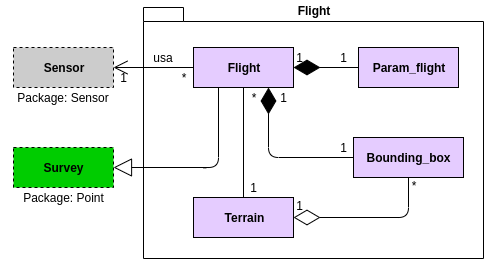
\includegraphics[width=1\hsize]{figuras/package_voo.png}
  %\legend{Texto da legenda quando necessário.}
  \source{A autora, 2019.}
\end{figure}

Neste modelo se adota o uso de um sensor para cada voo. A possibilidade de serem armazenados múltiplos sensores por voo pode ser adotada em uma extensão do modelo conceitual à ser realizada em trabalhos futuros. 

Os metadados desse sensor são armazenados no pacote \textbf{Sensor}, ilustrado na figura \ref{pack_sen}. Tem-se os dados do sensor conectados pela classe \textit{sensor}.

\begin{description}[labelwidth=2cm, itemsep=-0.3cm]
\item [Classe Sensor]
\item[Id:] Índice numérico;
\item[Id\_spec:] Referência para a classe \textit{Specification}; 
\item[Desc:] Descrição que o usuário pode usar para diferenciar seus sensores. 
\end{description}

Cada sensor possui especificações atreladas.  A classe \textit{Specification} contém essas informações. Note-se que as especificações de diversos sensores podem ser iguais se forem adotados equipamentos distintos de um mesmo modelo e fabricante. Tais valores são comuns aos diferentes equipamentos. Pequenas variações detectáveis em processos de calibração serão isolados em outra classe.

\begin{description}[labelwidth=2cm, itemsep=-0.3cm]
\item [Classe Specification]
\item[Id:] Índice numérico;
\item[Brand:] Modelo do sensor; 
\item[Manufact:] Fabricante do sensor;
\item[Focal:] Distância focal nominal da câmara em mm;
\item[Pixel\_size:] Tamanho do pixel no sensor; 
\item[Rows:] Quantidade de linhas do sensor;
\item[Cols:] Quantidade de colunas do sensor;
\item[Detector:] Identificador do tipo de sensor;
\end{description}

O atributo `\textit{Detector}' define se as imagens geradas pelo sensor serão de origem digital, ou analógica. Para tanto foi criado um \textit{data type}, ilustrado pela figura \ref{typesensor} do apêndice \ref{ap0}, que permite o armazenamento no banco justamente destes tipo enumerado.

Devido as pequenas variações a que estão submetidos os parâmetros internos do sensor por questões construtivas ou devido ao estresse de operação, não se recomenda a execução do processamento fotogramétrico sem os dados presentes no certificado de calibração. Tais dados podem ainda variar ao longo do tempo, motivo pelo qual uma data de validade de vinculada. Isto transmite a noção de que um mesmo sensor poderá ter diferentes calibrações, configurando a composição ``um para muitos'' entre a classe \textit{Sensor} e a classe \textit{Calibration} expressa a seguir. 

\begin{description}[labelwidth=2cm, itemsep=-0.3cm]
\item [Classe Calibration]
\item[Id:] Índice numérico;
\item[Id\_sensor:] Referência para a classe \textit{Sensor};
\item[Date\_cria:] Data de criação; 
\item[Date\_end:] Data de expiração;
\item[Number:] Número de série do certificado;
\item[Focal\_clb:] Focal calibrada da câmara em mm; 
\item[S\_focal\_clb:] Desvio-padrão da focal calibrada;
\item[Ppx:] Coordenada X do ponto principal do sensor em mm;
\item[Ppy:] Coordenada Y do ponto principal do sensor em mm;
\item[S\_ppx:] Desvio-padrão da coordenada X do ponto principal do sensor;
\item[S\_ppy:] Desvio-padrão da coordenada Y do ponto principal do sensor;
\item[Id\_sym:] Referência para classe \textit{Symmetric\_distortion};
\item[Id\_dec:] Referência para a classe \textit{Decentering\_distortion}.
\end{description}

Como o acervo comporta inúmeras imagens de origem analógica, as propriedades de câmaras métrica de formato analógico devem ser suportadas. Isso implica no registro de informações sobre as marcas fiduciais que são normalmente conferidas no processo de calibração. Por tanto, é esperado que a classe \textit{ficucials} represente um conjunto de informações que servirá apenas para vincular informações dos sensores analógicos.

\begin{description}[labelwidth=2cm, itemsep=-0.3cm]
\item [Classe Fiducials]
\item[Id:] Índice numérico;
\item[Id\_calib:] Referência para a classe \textit{Calibration};
\item[X:] Coordenada X em mm;
\item[Y:] Coordenada Y em mm; 
\item[Sigma\_x:] Desvio-padrão da coordena X;
\item[Sigma\_y:] Desvio-padrão da coordenada Y.
\end{description}

Ao capturar uma imagem, o feixe de luz pode sofrer desvios (como visto no item \ref{sensofot}). Duas das distorções que afetam a posição dos objetos imageados, são chamadas de radial simétrica e descentrada. Soluções matemáticas, dadas pelos sistemas de equações \ref{sim1} e \ref{des1}, ambos precisam de dados que são informados no certificado de calibração. As classes \textit{Symmetric\_distortion} e  \textit{Decentering\_distortion} conectam esse dados ao certificado de calibração. 

O modelo adotado para a distorção radial simétrica é: 

\begin{equation} \label{sim1}
\begin{array}{cl}
\delta x &= (k0 + k1r^{2} +k2r^{4} +k3r^{6})x" \\
\delta y &= (k0 + k1r^{2} +k2r^{4} +k3r^{6})y" \\
x' &= x'' - \delta x \\
y' &= y'' - \delta y
\end{array}
\end{equation}

Onde:

$\delta$x, $\delta$y: componentes da distorção radial simétrica;

r é o raio a partir do ponto principal de simetria;

k0, k1, k2, k3: coeficientes do certificado de
calibração;

x”, y”: coordenadas do ponto sem correção, referidas ao ponto principal de simetria;

x’, y’: as coordenadas corrigidas da distorção radial simétrica.

\begin{description}[labelwidth=2cm, itemsep=-0.3cm]
\item [Classe Symmetric\_distortion]
\item[Id:] Índice numérico;
\item[Id\_calib:] Chave estrangeira que faz referência ao atributo `Id' da classe `Calibration';
\item[K0:] Coeficiente k0 de distorção da lente;
\item[K1:] Coeficiente k1 de distorção da lente;
\item[K2:] Coeficiente k2 de distorção da lente;
\item[K3:] Coeficiente k3 de distorção da lente; 
\item[Sigma\_k0:] Desvio-padrão do coeficiente k0;
\item[Sigma\_k1:] Desvio-padrão do coeficiente k1;
\item[Sigma\_k2:] Desvio-padrão do coeficiente k2;
\item[Sigma\_k3:] Desvio-padrão do coeficiente k3.
\end{description}

A distorção descentrada é resolvida, por sua vez, adota as formulações: 

\begin{equation} \label{des1}
\begin{array}{cl}
\delta x' &= p1(r^{2}+x"^{2})+p2r^{2}x"^{2}y"^{2} \\
\delta y' &= p1(r^{2}+y"^{2})+p2r^{2}x"^{2}y"^{2} \\ 
x &= x' - \delta x'\\
y &= y' - \delta y'
\end{array}
\end{equation}

Onde:

$\delta$x', $\delta$y': componentes da distorção radial descentrada;

r é o raio a partir do ponto principal de simetria;

p1, p2: coeficientes do certificado de calibração;

x”, y”: coordenadas do ponto sem correção, referidas ao ponto principal de simetria;

x’, y’: coordenadas corrigidas da distorção radial descentrada;

x, y: coordenadas corrigidas das duas distorções.

\begin{description}[labelwidth=2cm, itemsep=-0.3cm]
\item [Classe Decentering\_distortion]
\item[Id:] Índice numérico;
\item[P1:] Coeficiente P1 de distorção da lente;
\item[P2:] Coeficiente P2 de distorção da lente; 
\item[Sigma\_p1:] Desvio-padrão do coeficiente p1;
\item[Sigma\_p2:] Desvio-padrão do coeficiente p2.
\end{description}

\begin{figure}[!ht]{13cm}
  \caption{Pacote Sensor} \label{pack_sen}
  \centering
  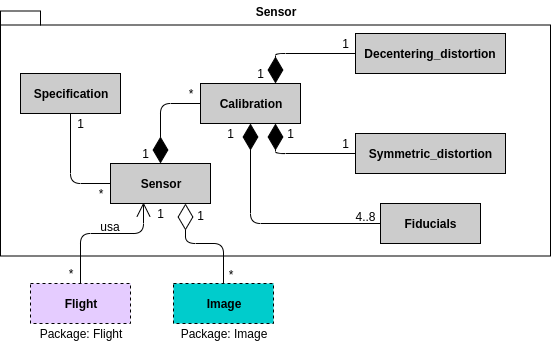
\includegraphics[width=1\hsize]{figuras/package_sensor.png}
  %\legend{Texto da legenda quando necessário.}
  \source{A autora, 2019.}
\end{figure}

Na etapa `Aquisição e Cadastro de Dados' do item \ref{efoto} se gerados os dados dos pacotes \textbf{Image} e \textbf{Point}. Como algumas classes de imagem mencionam algumas informações pertencentes às classes de pontos, decidiu-se apresentar o último antes do primeiro, evitando assim que houvesse a necessidade da quebra da imagem na apresentação adotada neste trabalho para tal pacote. Isso é dito pois, o levantamento topográfico normalmente é feito depois da captação das fotografias aéreas.

\textit{Point} é a classe principal do pacote de mesmo nome. A obtenção de seus dados são a razão pelo qual um levantamento topográfico é realizado. Esta classe possui dados geográficos. Por tanto pode ser usada com um exemplo claro da presença de dados complexos no modelo e a necessidade de trabalhar com um banco que possua extensões para dados geográficos. Adotar tal recurso permite indexação e consequente aceleração nas buscas por pontos numa dada região de interesse quando isto for de interesse dos usuários do banco de dados sob desenvolvimento.

%Figura \ref{point}: \textbf{Classe Point}
\begin{description}[labelwidth=2cm, itemsep=-0.3cm]
\item [Classe Point]
\item[Id:] Índice numérico;
\item[Name:] Nome do ponto;
\item[Geom:] Coordenadas tridimensionais do ponto (pointz);
\item[Sigma:] Desvio-padrão das coordenadas do ponto;
\item[Id\_coll:] Referência para a classe \textit{Collection}.
\end{description}

Vários pontos formam uma coleção de pontos. Um levantamento topográfico pode ser feito em dias distintos, ou seja, podem possuir várias coleções de pontos. Ao mesmo tempo, um projeto fotogramétrico pode selecionar subconjuntos de pontos nas diferentes coleções disponíveis de levantamentos topográficos na região de interesse do projeto fotogramétrico. Estas associações requerem tabelas de associação e para explicitá-las foram estipuladas as classes de ligação \textit{Collection\_point} e \textit{Point\_project} respectivamente.

\begin{description}[labelwidth=2cm, itemsep=-0.3cm]
\item [Classe Collection\_Point]
\item[Id:] Índice numérico;
\item[Id\_srs:] Referência para a classe \textit{Srs};
\item[Date:] Data da coleta da coleção de pontos;
\item[Receptor:] Receptor da antena;
\item[Antenna:] Antena usada no levantamento;
\item[Ant\_lvl:] Altura da antena em m;
\item[Id\_survey:] Referência para a classe \textit{Ground\_survey}.
\end{description}

É importante notar que esta classe tem uma coloração diferente do resto no pacote. Este destaque foi usado para destacar a entidade associativa que liga duas classes principais e, por consequência, dois pacotes.  

\begin{description}[labelwidth=2cm, itemsep=-0.3cm]
\item [Classe Point\_project]
\item[Id\_proj:] Referência para a classe \textit{Project};
\item[Id\_point:] Referência para a classe \textit{point};
\item[Use:] Função que o ponto está exercendo no projeto fotogramétrico.
\end{description}

O mesmo ponto pode ser de controle, fotogramétrico ou usado como ponto de verificação. Seu uso varia de acordo com o projeto que se esta trabalhando. Para definir esse uso, foi criado um \textit{data type} específico, apresentado na figura \ref{pointype} do apêndice \ref{ap0}.

Por último, na classe \textit{Ground\_survey} do pacote \textbf{Point}, representado na figura \ref{pack_point}, se encontram os metadados do levantamento topográfico. 

\begin{description}[labelwidth=2cm, itemsep=-0.3cm]
\item [Classe Ground\_survey]
\item[Id:] Índice numérico;
\item[Id\_Survey:] Referência para a classe \textit{Survey};
\end{description}

\begin{figure}[!ht]{13cm}
  \caption{Pacote Point} \label{pack_point}
  \centering
  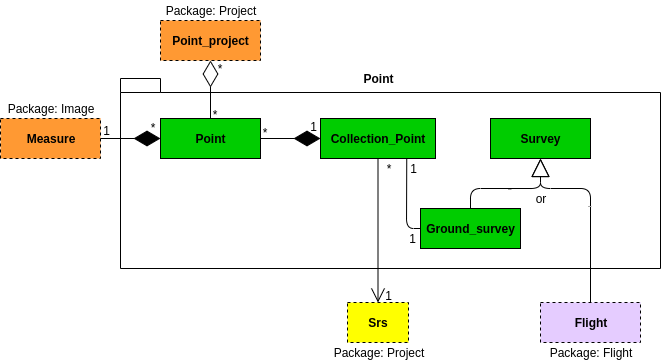
\includegraphics[width=1\hsize]{figuras/package_point.png}
  %\legend{Texto da legenda quando necessário.}
  \source{A autora, 2019}
\end{figure}

O último pacote a ser apresentado é o pacote \textbf{Image}. Foram modelados e implementados, até o momento da defesa deste trabalho, os dados relacionados às imagens geradas a partir de um aerolevantamento. O uso de fotos analógicas deve prever a digitalização deste materiais para permitir o processamento digital pelas ferramentas de software disponíveis no LFSR.

Marcas fiduciais, nas fotos de câmaras métricas, bem como, pontos no terreno são associados as imagens através do processo de medição. Assim obtém-se para cada ponto existente no terreno (espaço-objeto) um conjunto de medidas análogas (no espaço-imagem), em \textit{pixels}. A classe \textit{measure} realiza a analogia entre tais sistemas de coordenadas.

\begin{description}[labelwidth=2cm, itemsep=-0.3cm]
\item [Classe Measure]
\item[Row:] Número da linha em que se encontra o pixel;
\item[Col:] Número da linha em que se encontra o pixel;
\item[Id\_img:] Referência para a classe \textit{Image};
\item[Id\_point:] Referência para a classe \textit{Point};
\item[Id\_proj:] Referência para a classe \textit{Project}.
\end{description}

A classe principal deste pacote é a classe \textit{image} que contém os metadados do fotograma digitalizado ou da fotografia digital. 

\begin{description}[labelwidth=2cm, itemsep=-0.3cm]
\item [Classe Image]
\item[Id:] Índice numérico;
\item[Name:] Nome da imagem;
\item[Resolution:] Resolução da imagem;
\item[Size\_pixels:] Resolução da imagem em numero de linhas e colunas de pixels;
\item[Img\_type:]  Define o tipo de imagem armazenada (para diferenciar ortoimagens em extensões);
\item[Id\_sensor:]  Referência para a classe \textit{Sensor};
\item[Id\_strip:] Referência para a classe \textit{Strip}.
\end{description}

Como se trata de um modelo de banco de dados voltado para o acervo de um laboratório, um dos dados mais importantes é a armazenagem dos arquivos digitais das imagens. Este modelo prevê duas formas de armazenamento: por caminho de onde se encontra o arquivo no servidor físico; ou pelo armazenamento do próprio arquivo como um \textit{Raster} dentro do banco. Este último só é possível se o banco possuir uma extensão geográfica que comporte tal tipo de arquivo. Estes armazenamentos modelados com a previsão das classes \textit{file\_img} e \textit{Tn}. 

\begin{description}[labelwidth=2cm, itemsep=-0.3cm]
\item [Classe File\_img]
\item[Id\_img:]  Referência para a classe \textit{Image};
\item[File\_path:] Caminho no servidor para o arquivo da imagem;
\item[Table:] Nome da tabela onde se encontra armazenada a imagem no banco;
\end{description}

As classes modeladas até este momento tem implementação no banco como tabelas. Deste modo, cada classe deve gerar uma tabela e cada objeto instanciado terá seu requisito de persistência atendido por uma tupla, motivo pelo qual foram expostas classes de associação.

A classe \textit{Tn}, por particularidades de implementação de diversas aplicações de SIG, adotará um esquema isolado no banco no qual cada imagem será armazenada por uma tabela distinta. Isto justifica-se pela possibilidade de cada tabela do banco ser tratada como uma camada de informação nos SIGs, ou seja, a carga de imagens isoladas será mais conveniente por intermédio deste recurso.

Decidiu-se padronizar o nome das tabelas que representam instâncias da classe \textit{Tn}, onde `T' se refere a table e `n' deve ser substituído pelo valor do atributo `Id' de sua tupla correspondente na classe `Image'. Prevendo a possibilidade desse armazenamento poder ser parametrizado para ocorrer em um banco dedicado, o atributo `Table' deve conter o nome da tabela do raster com o prefixo de nome do esquema, ou seja, `schema.Tn', por exemplo: 'img.T1'.

\begin{description}[labelwidth=2cm, itemsep=-0.3cm]
\item [Classe Tn]
\item[rid:] Índice numérico;
\item[rast:] Arquivo binário da imagem.
\end{description}

Devido à forma de carga realizada, os atributos dessa última classe seguem os padrões adotados pela biblioteca GDAL que será discutido posteriormente.

A classe \textit{Photo} define forma pela qual essa imagem foi obtida. Como está se trata da modelagem de um processo de aerofotogrametria tradicional, com sensores analógicos, a geometria esperada é a de `quadro a quadro'. Prevendo futuras expansões que incluam a obtenção por outros tipos de sensores, esta geometria admite outras formas de captação de imagem. Para isso foi estabelecido um \textit{data type} específico, chamado \textit{Typephoto}, presente na figura \ref{tp} do apêndice \ref{ap0}, que comportasse essas geometrias. Todas as opções do mesmo, exceto `frame', são exemplo de como estas geometrias se encaixariam no modelo, pois não são contempladas atualmente no modelo quanto a formulação matemática necessária para a parametrização de suas orientações (interior e exterior).

\begin{description}[labelwidth=2cm, itemsep=-0.3cm]
\item [Classe Photo]
\item[Id:] Índice numérico;
\item[Geom\_t:] Tipo de geometria da imagem.
\end{description}

Atrelada à classe \textit{Frame} estão os metadados restantes da fotografia como a possibilidade de referência para informações de inicialização dos ângulos de atitude e posicionamento do sensor representados, respectivamente, por objetos das classes \textit{Frame\_gnss} e \textit{Frame\_ins}.

\begin{description}[labelwidth=2cm, itemsep=-0.3cm]
\item [Classe Frame]
\item[Id\_img:]  Referência para a classe \textit{Image};
\item[Num\_neg:] Número da foto no negativo.
%\item[Geom:] Polígono da projeção desta fotografia no terreno;
\item[Id\_block:]  Referência para a classe \textit{Block};
\item[Id\_gnss:]  Referência para a classe \textit{Frame\_gnss};
\item[Id\_ins:]  Referência para a classe \textit{Frame\_ins}.
\end{description}

A sequencia de imagens em uma linha de voo é chamada de faixa e seu conjunto conhecido como bloco. As classes \textit{Strip} e \textit{Block} armazenam as informações de faixas e blocos respectivamente.

\begin{description}[labelwidth=2cm, itemsep=-0.3cm]
\item [Classe Strip]
\item[Id:] Índice numérico;
\item[Name:] Nome da faixa;
\item[Id\_block:]  Referência para a classe \textit{Block}.
\end{description}

\begin{description}[labelwidth=2cm, itemsep=-0.3cm]
\item [Classe Block]
\item[Id:] Índice numérico;
\item[Id\_proj:]  Referência para a classe \textit{Project}.
\end{description}

Admite-se que todo projeto possui se consolida pela escolha de um bloco e que o conhecimento prévio da estruturação do mesmo é fator fundamental para o sucesso. Contudo, quando não for possível estabelecer de imediato a estruturação hierárquica, de imagens em faixas e faixas no bloco, pelo intermédio de um fotoíndice ou qualquer outro recurso, a classe associativa \textit{img\_block} proverá a ligação necessária para informar que o projeto fez agregação da imagem. Em outras palavras, este último se refere a coleção de imagens com que um projeto fotogramétrico escolhe trabalhar. Isso significa que um projeto fotogramétrico pode trabalhar com apenas parte do bloco de um aerolevantamento e, salvo as dificuldades organizacionais, com blocos não estruturados e sem faixas bem definidas.

\begin{description}[labelwidth=2cm, itemsep=-0.3cm]
\item [Classe Img\_block]
\item[Id\_img:]  Referência para a classe \textit{Image}.
\item[Id\_block:]  Referência para a classe \textit{Block}.
\end{description}

Para garantia das buscas de dados, recomenda-se que mesmo projetos estruturados, gerem os registros de seleção na classe associativa entre imagem e bloco. A redundância de referências aqui, bem como a manutenção de sua integridade, pode ser garantida pela implementação de gatilhos no banco após sua implementação.

O rodapé da imagem pode ser tomado como recurso útil para destacar também os chamados `pares de imagens'. Basicamente, se duas imagens possuem sobreposição ao registrar um mesmo espaço no terreno, isto pode ser investigado com os recursos de análise espacial presentes nos SGBDs espaciais. O cadastramento de pares de imagens é feito pela classe \textit{Pair}. 

\begin{description}[labelwidth=2cm, itemsep=-0.3cm]
\item [Classe Pair]
\item[Id\_c\_cov:]  Referêcia para a classe \textit{Common\_coverage};
\item[Id\_img1]  Referência para o primeiro objeto da classe \textit{Image} no par;
\item[Id\_img2]  Referência para o segundo objeto da classe \textit{Image} no par.
\end{description}

Contudo, para se determinar um par, se depende da projeção geométrica do polígono correspondente desta imagem no terreno. A classe \textit{Coverage} armazena estes dados.

\begin{description}[labelwidth=2cm, itemsep=-0.3cm]
\item [Classe Coverage]
\item[Id\_img]  Referência para a classe \textit{Image};
\item[Gsd:] Tamanho do pixel no terreno (em metros);
\item[Geom:] Polígono da projeção da imagem no terreno.
\end{description}

A existência de um par implica que existe uma interseção entre duas imagens. Esta interseção pode, ou não, pertencer à um `par estereoscópico' na mesma faixa, porém a estereoscopia depende do tipo de imagem. Se o modelo for estendido para comportar produtos como, por exemplo, as ortoimagens, então estas não atenderão aos requisitos para formação de um par estereoscópico, mesmo que este par possua interseção. Isto é justificado, uma vez que a estereoscopia é fenômeno que depende da intersecção de feixes luminosos  e estes serão `aproximadamente' paralelos nas ortoimagens. A classe \textit{Common\_coverage} pode armazenar a verificação destas restrições, sob a forma de dois principais atributos: um \textit{booleano} para determinar se é possível realizar estereoscopia; e uma geometria que permita preservar o resultado de operações de intersecção das regiões cobertas por imagens.

\begin{description}[labelwidth=2cm, itemsep=-0.3cm]
\item [Classe Common\_coverage]
\item [Id:] Índice numérico;
\item [Intersection:] Interseção entre polígonos das imagens;
\item [Stereoscopy:] Estereoscopia na interseção das imagens.
\end{description}

Uma imagem pode ser sobreposta por `n' outras imagens, assim ocorrendo `n' interseções de imagens sobre esse mesmo espaço. Para estes casos foram modeladas as classes \textit{Ntuplet} e \textit{Img\_ntuplet}, que generalizam o conceito de `par' para prover suporte ao reconhecimento de quais regiões do terreno possuem coberturas com sobreposição de números de imagens superiores a duas e, quais imagens participam destas sobreposições múltiplas, respectivamente. 

\begin{description}[labelwidth=2cm, itemsep=-0.3cm]
\item [Classe Ntuplet]
\item[Id:] Índice numérico;
\item[Id\_c\_cov:]  Referência para a classe \textit{Common\_coverage}.
\item[Size:] Quantidade de imagens que fazem interseção com a região de interesse;
\end{description}

\begin{description}[labelwidth=2cm, itemsep=-0.3cm]
\item [Classe Img\_ntuplet]
\item[Id\_ntuplet:] Referência para a classe Ntuplet;
\item[Id\_img:]  Referência para a classe \textit{Image}.
\end{description}

O arquivo digital do fotograma não possui métrica, tendo associado somente coordenadas por pixels de forma isolada. Para corrigir isso é realizada a correção dos feixes perspectivos, comumente conhecida como Orientação Interior (OI). A OI basicamente reconstrói o sistema interno câmara-imagem da fotografia para o momento em que a mesma foi tirada. A equação \ref{oi1} resume o modelo paramétrico usado para a OI.

\begin{equation} \label{oi1}
\begin{cases}
x=a_{0}+a_{1}.coluna+a_{2}.linha\\
y=b_{0}+b_{1}.coluna+b_{2}.linha
\end{cases}
\end{equation}

Onde:

$x$ e $y$: Coordenadas das marcas fiduciais;

$linha$ e $coluna$: Coordenadas das marcas fiduciais do certificado de calibração;

$a0$, $a1$, $a2$, $b0$, $b1$ e $b2$: Parâmetros de transformação entre os sistemas.

A partir do momento em que se tem a OI, o próximo passo é a realização da orientação exterior (OE). Esta por sua vez, obtém a posição e os ângulos de atitude do momento de registro da cada fotografia. A OE dera de seis parâmetros, independentemente do procedimento que usa para ser obtida. Estes são ilustrados na figura \ref{atitude}.

\begin{figure}[!ht]{8cm}
  \caption{Objetos da OE} \label{atitude}
  \centering
  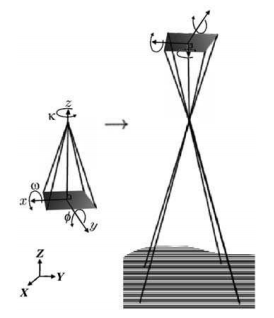
\includegraphics[width=1\hsize]{figuras/atitude.png}
  %\legend{Texto da legenda quando necessário.}
  \source{\cite{coelho2007fotogrametria}}
\end{figure}

Assim,

$\phi$, $\omega$, $\kappa$: Ângulos de Euler, chamados de ângulos de atitude;

$X0$, $Y0$ e $Z0$: Coordenadas no espaço-objeto para o CP da tomada da foto.

O ângulo $\phi$ que corresponde a rotação em relação ao eixo Y, o ângulo $\omega$ que corresponde a rotação em relação ao eixo X e o ângulo $\kappa$ que corresponde a rotação em relação ao eixo Z. Os ângulos de atitude para cada foto registram a angulação de inclinação do avião na hora da tomada da foto.

Uma vez realizada a orientação interior e exterior de uma imagem é possível a obtenção das coordenadas tridimensionais de um ponto na imagem em sua posição correspondente no terreno. A presença dos valores de seus parâmetros caracteriza a etapa de inicialização do processo fotogramétrico como concluída. Assim decidiu-se registrar no modelo de banco a presença dos modelos paramétricos adotados pelas orientações, interior e exterior, bem como seus parâmetros e coeficientes computados por projeto. Os procedimentos e seus parâmetros podem ser armazenados nas classes \textit{Mod\_param}, \textit{Parameter}, \textit{Coef\_img} e \textit{Processing\_metho}.

\begin{description}[labelwidth=2cm, itemsep=-0.3cm]
\item [Classe Mod\_param]
\item[Id:] Índice numérico;
\item[Type:]  Tipo de de operação realizada.
\item[Num\_par:] Quantidade de parâmetros de interesse;
\item[Name:] Nome da operação;
\item[Formula:] Equação e/ou modelo matemático utilizado para o cálculo da operação.
\end{description}

Para que a classe \textit{Mod\_param} se comunique melhor com a classe  \textit{parameter} foi criado o \textit{data type} \textit{type\_op} (figura \ref{top} nos apêndices), onde o tipo de procedimento realizado é previsto.

\begin{description}[labelwidth=2cm, itemsep=-0.3cm]
\item [Classe Parameter]
\item[Id:] Índice numérico;
\item[Sequential:] Número de um ordem sequencial estabelecida para o parâmetro;
\item[Name:] Nome do parâmetro;
\item[Symbol:] Simbolo que represente o parâmetro;
\item[Id\_mpar:] Referência para a classe \textit{Mod\_param}.
\end{description}

\begin{description}[labelwidth=2cm, itemsep=-0.3cm]
\item [Classe Coef\_img]
\item[Id:] Índice numérico;
\item[Id\_img:] Referência para a classe `Image’;
\item[Id\_proj:] Referência para a classe `Project';
\item[Value:] Valor do coeficiente gerado; 
\item[Id\_pmet:]  Referência para a classe `Processing\_metho'.
\end{description}

\begin{description}[labelwidth=2cm, itemsep=-0.3cm]
\item [Classe Processing\_method]
\item[Id:] Índice numérico;
\item[Data\_origin:] Tipo de procedimento q gera o coeficiente.
\end{description}

Os parâmetros da orientação exterior de uma imagem podem ser fornecidos por intermédio de sistemas auxiliares, tais como GNSS, para o cálculo das coordenadas do CP, e pelos Sistemas de Navegação e medição inerciais, situação na qual são fornecidos os ângulos de atitude do sensor no instante de cada tomada fotográfica. Para o primeiro caso foi criada a classe \textit{frame\_gnss}, para o segundo, \textit{frame\_ins}. Ambas as classes possuem um atributo booleano chamado `status'. Se o mesmo for nulo assumi-se que estes valores são desconhecidos e logo a tupla não existirá. Se este valor for verdadeiro, então tem-se que os dados são `fixos'. Se o valor for falso entende-se que esses valores são `iniciais'.

\begin{description}[labelwidth=2cm, itemsep=-0.3cm]
\item [Classe Frame\_gnss]
\item[Id:] Índice numérico;
\item[Status:] Indicador booleano do status dos dados de entrada;
\item[Geom:] Coordenadas de entrada do CP da imagem;
\item[Sigma\_E:] Desvio-padrão da coordenada E;
\item[Sigma\_N:] Desvio-padrão da coordenada N;
\item[Sigma\_H:] Desvio-padrão da coordenada H;
\end{description}

\begin{description}[labelwidth=2cm, itemsep=-0.3cm]
\item [Classe Frame\_ins]
\item[Id:] Índice numérico;
\item[Status:] Indicador booleano do status dos dados de entrada;
\item[Omega:] Ângulo de atitude $\omega$ de entrada da imagem;
\item[Phi:] Ângulo de atitude $\phi$ de entrada da imagem;
\item[Kappa:] Ângulo de atitude $\kappa$ de entrada da imagem;
\item[S\_omega:] Desvio-padrão do angulo $\omega$;
\item[S\_phi:] Desvio-padrão do angulo $\phi$;
\item[S\_kappa:] Desvio-padrão do angulo $\kappa$;
\end{description}

A figura \ref{pack_img} apresenta como estas classes interagem se comunicam.

\begin{landscape}
\begin{figure}[ht]{23cm}
  \caption{Pacote Image.} \label{pack_img}
  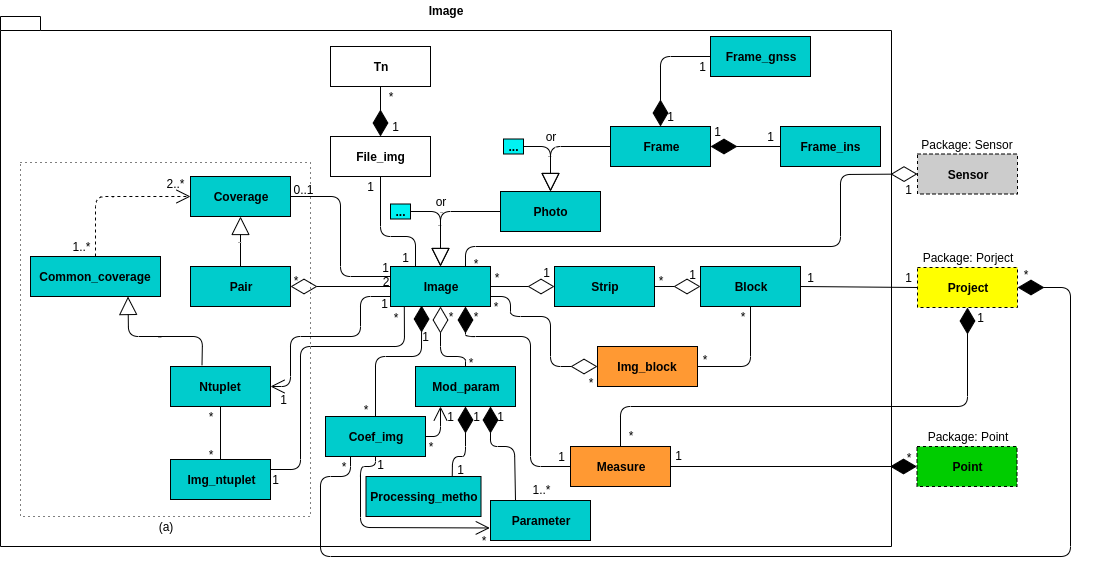
\includegraphics[width=\hsize]{figuras/package_img.png}
  \legend{(a) conjunto de classes que podem se tornar um sub-pacote.}
  \source{A autora, 2019}
\end{figure}
\end{landscape}

%Essa subseção gera em anexo modelos, LEMBRAR: de disponibilizar também o arquivo digital, não somente a imagem impressa (deixando isso bem claro no trabalho)
Não se entrou em detalhes quanto ao produtos finais de um projeto fotogramétrico. Isso se dá pelo fato de que para o pacote produto a variedade de variáveis e possíveis produtos é tão complexa que se optou neste trabalho por não mapeá-los no modelo. Vale ressaltar que em alguns momentos o modelo deixa indicado onde possíveis extensões podem ocorrer, inclusive os produtos ortofoto e por consequência ortomosaico. Porém deve ser deixar claro que nenhum produto final é contemplado no modelo conceitual. A extensão do mesmo com a inclusão do pacote de produtos é um possível futuro trabalho a ser realizado.

O modelo com todas classes e suas conexões detalhado é grande e complexo, de modo que foi optado por não inseri-lo no texto. O mesmo se encontra apresentado na figura \ref{modelo_00} no apêndice \ref{ap-1}. Um arquivo digital da imagem deste modelo será disponibilizado para que assim seja possível uma leitura do modelo como um todo.

Desde a primeira versão até a versão final apresentada neste texto, o modelo orientado a a objeto sofreu diversas modificações. Três meses após o início da modelagem percebeu-se que o método de processo de desenvolvimento monolítico, até então utilizado, corria o risco de não se cumprir o prazo estabelecido. Isso acarretou na transição para o método de processo de desenvolvimento ágil. Até aquele momento o modelo havia sido trabalhado com apoio da fundamentação teórica. A partir daquele momento, houve a preocupação da geração de um código base, implementação de um banco de dados usando esse código e a realização de testes que verificassem a integridade técnica do banco. 

O código base, do qual se implementaria um banco de dados baseado neste modelo deveria ser gerado automaticamente pela ferramenta utilizada para desenhar o mesmo. A ferramenta escolhida foi o Umbrello. Isso aconteceu pois a ferramenta em questão atende a linguagem UML 2.0, e e capaz de gerar um código em sql a partir do modelo desenhado. Outras ferramentas no mercado, de conhecimento da autora, são pagas ou não comportam as necessidades do modelo devido sua complexidade. Dentre essas ferramentas, existem plataformas que trabalham com as linguagens de Geoframe e OMT-G, o que implicou na escolha da linguagem UML 2.0. O problema encontrado foi que o sql gerado a partir do modelo desenhado possui uma quantidade de erros e inconsistências considerada demasiadamente alta, o que tornava o código inviável para utilização. A solução pensada foi a tradução do modelo até então trabalhado para um modelo relacional. Dessa forma, agora num processo ágil, toda mudança realizada no código por causa de testes, agora afetava o modelo relacional e o modelo orientado a objeto.


\subsection{Modelo Relacional}

Apesar do que foi citado no item \ref{sgbdr}, a despeito do que informa Korth, foi necessária adaptação de parte da modelagem OO realizada para um Modelo Relacional. Utilizando a ferramenta online ERDplus, adaptações foram realizadas. Heranças do modelo orientado objeto viraram \textit{constrains} sequenciais de FK no modelo relacional. Os dados complexos que até o momento tinham tipos específicos, viraram tipos alfanuméricos. Modificações no código então se fizeram necessárias. Essa modificações só foram possíveis pois já que o banco seria codificado como relacional, optou-se por escolher um banco que possuísse uma extensão geográfica. Assim gerando um código base que implementasse um banco objeto relacional.

Devido a seus tamanho junto ao fato de que todas as suas classes foram apresentadas anteriormente, optou-se por não colocar o modelo no texto deste documento. Porém o mesmo encontra-se na figura \ref{modelo_r} do apêndice \ref{ap-1}.

O modelo relacional foi usado como um `gap' que permitisse a geração do código de forma a otimizar o tempo disponível. A utilização do mesmo resultou na implementação de um banco de dados objeto relacional.



\section{Implementação do Projeto Piloto}

O software aplicativo de banco de dados escolhido para a implementação do modelo foi o PostgreSQL. Devido à sua capacidade de armazenar e manipular dados geográficos, utiliza-se também da extensão PostGIS. Todas as classes de estereótipo de dados geográfico apresentadas no modelo, \textbf{point}, \textbf{polygon} e \textbf{raster}, precisaram utilizar em sua programação e carga comandos específicos. Este só foram possíveis pela utilização da extensão espacial no banco. A figura \ref{postpost} ilustra esta integração.

\begin{figure}[!ht]{10cm}
  \caption{Integração PostgreSQL e Postgis} \label{postpost}
  \centering
  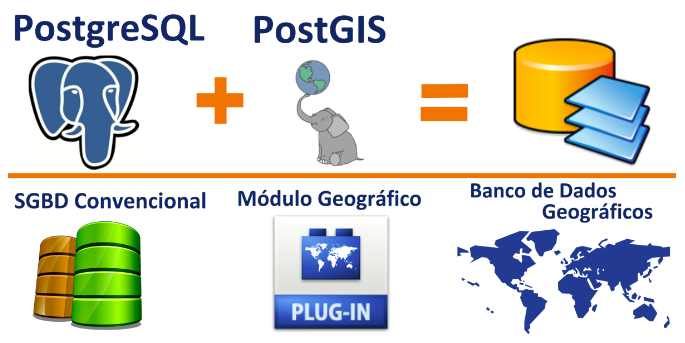
\includegraphics[width=1\hsize]{figuras/postgre_postgis.png}
  %\legend{Texto da legenda quando necessário.}
  \source{\cite{clickgeosgbd}}
\end{figure}

A codificação de criação das estruturas do banco não necessariamente precisa de uma interface. Por questões de familiaridade da autora com a plataforma optou-se por fazer a implementação do mesmo por uma interface de administração do SGBD. A interface escolhida foi o PgAdmin III.

A grande maioria dos testes de verificação e validação realizados neste trabalho foram feitos por processos de \textit{query} usando a linguagem sql. A `query' pode ser entendida como pedido, consulta, solicitação ou requisição de informações ou dados presentes num banco, utilizando um código pré-definido. Neste caso o código é o sql, como previamente comentado.

O código de geração das tabelas e tipos de dados do projeto piloto se encontra no apêndice \ref{ap1}. Este contém 446 linhas, compostas de códigos e comentários feitos em sql. O código foi feito em cascata, com exceção de uma pequena parte ao final desse código. Dessa forma, basicamente todas as tabelas presentes no banco são criadas em conjunto a criação de seu esquema. Isso resulta que ao utilizar o código disponível neste documento, a criação do banco é realizada quase que de uma só vez. Faltando somente a criação das tabelas responsáveis pelo armazenamento das fotografias no banco de dados. Este caso particular será apresentado ao final da próxima seção. 



\section{Carga}\label{cargs}

Com o código base gerado, o tipo de banco escolhido e as modificações necessárias para que esse código pudesse armazenar os dados geográficos no banco, o próximo passo foi a implementação do banco de dados piloto.

Como o código inicial era extenso, o mesmo foi `quebrado' à medida que foi testado e implementado. Cada tabela foi testada sozinha, de forma a verificar a sintaxe do código. Quando uma tabela passava no teste, a seguinte era acoplada ao código trabalhado. O novo segmento de código, agora contando as partes verificadas e uma tabela não testada era testado novamente, verificado, e corrigido se necessário. Esse processo era repetido até que o novo código passasse pelo teste e pudesse ser adicionado à uma nova parte do código base.  Assim entrou-se num processo em loop de testes, correções e acréscimos ao código que em muito se assemelha ao processo TDD, explicado no item \ref{proc}. A principal diferença é que um processo TDD é desde seu início um processo ágil, enquanto este trabalho começou como um processo monolítico, antes de migrar para o processo ágil. Assim não se pode dizer que o trabalho siga o modelo TDD, e sim que se aproxima do mesmo. Toda correção que não fosse de sintaxe, gerava alterações nos modelos, tanto no relacional quanto no orientado a objeto. Assim, houve uma correção constante de ambos os modelos, de forma a não se perder detalhes do processo. Ao final, o banco gerado foi apagado para que numa última bateria de testes do código fosse implementada por inteiro. Essa fase de implementação e testes foi, o que se pode entender como a primeira fase de verificação. A partir deste momento tinha-se um banco implementado e aparentemente verificado. Novamente realizando testes, começou-se a realizar 'cargas' por cada tabela no banco. Iniciou-se então um novo loop. Agora o objetivo não era só saber se o banco funcionava, mas sim se ele suportava os dados fornecidos pelo LFSR. Entra-se então na segunda fase de verificação com testes, erros, correções e incrementos do código. A diferença é que nesta segunda bateria de testes, a expectativa era de uma quantidade menor de erros. Em compensação, grande parte dos erros descobertos e corrigidos ao realizar essas cargas geravam modificações no código-base trabalhado, nos modelos e testes do próprio código. Um exemplo do exposto é a classe \textit{measure}, onde inicialmente não continha o atributo `Id\_proj', este por sua vez relaciona a medida do ponto na imagem à um projeto, assim evitando que medições de um mesmo ponto em uma mesma imagem se confundissem.

Todas as cargas foram feitas por meio de `querys', com exceção das necessárias para os arquivos ``raster'' das imagens. O código abaixo é exemplo de uma carga de dados alfanuméricos (parte do código presente no apêndice \ref{carga1}).

\begin{lstlisting}
INSERT INTO efoto.Fiducials (Id,x,y,Sigma_x,Sigma_y,Id_calib)
VALUES
('1','113','0.016',null, null,'1'),
('2','-113.006','0.018',null, null,'1'),
('3','0.004','113.015',null, null,'1'),
('4','0.007','-112.975',null, null,'1');
\end{lstlisting}

Nesta carga, foram armazenados na tabela `Fiducials' os valores das coordenadas das marcas fiduciais. Estes foram obtidos no certificado de calibração do sensor já armazenado no banco. Outro exemplo de carga é o realizado na tabela de pontos. 

O exemplo a seguir é parte de uma das cargas realizadas (o código da carga completa se encontra no apêndice \ref{carga2}).

\begin{lstlisting}
INSERT INTO efoto.Point (Id, Name_, Geom, Sigma, Id_coll)
VALUES
('14','LH1',ST_Transform(ST_GeomFromText('POINTZ(680947.997 7464833.669 3.942)',32723),4326),null,'7'),
('15','LH2',ST_Transform(ST_GeomFromText('POINTZ(680895.378 7463828.578 9.206)',32723),4326),null,'7'),
('16','LH3',ST_Transform(ST_GeomFromText('POINTZ(682227.162 7464200.581 2.184)',32723),4326),null,'7');
\end{lstlisting}

Diferentemente do primeiro exemplo, esta segunda carga possui dados complexos. Neste caso refere-se às coordenadas geográficas dos pontos armazenados.  Estes só puderam ser armazenados devido o uso da extensão Postgis. Para isto, foi utilizado o domínio `POINTZ', que permite o armazenamento de coordenadas 3D para pontos padronizado como um dado geográfico, que usa o EPSG:4326, ou seja, possui como sistema de referência geodésico o WSG 84. A principal diferença entre dados geográficos para dados geométricos para o Postgis é que o primeiro assume que os dados carregados são compostos por pontos na superfície da Terra, enquanto para os dados ditos geométricos se assume que estes dados se encontram num plano plano cartesiano, como uma projeção cartográfica. 
Como visto no exemplo, as coordenadas de entrada estão na projeção UTM, isso significa que devem ocorrer algumas transformações ao armazenar esses dados. Usando a função ``ST\_GeomFromText()'', é contruído um objeto geométrico baseado no WKT (well-know text) e no SRS (spacial reference system) de origem. A partir desse ponto é feita a conversão deste dado para o SRS do banco com a função ``ST\_Transform()''. O segmento do exemplo anterior, mostrado a seguir, possui as transformações explicadas:

\begin{verbatim}
    ST_Transform(ST_GeomFromText('POINTZ(680947.997
    7464833.669 3.942)',32723)
\end{verbatim}

Qualquer que seja o valor dos dados geográficos a ser armazenado em um banco de dados, deve-se considerar suas projeções e sistemas de referência. Logo, deve-se ter conhecimento de quais valores do índice do EPSG, e se necessário, quais transformações serão necessários para a realização do armazenamento correto de tais dados.

Foram realizadas 3 cargas de grupos de dados. A primeira consistindo dos dados do projetos `UERJ-OI',`UERJ-OI-OE' e `UER-no-orient' disponíveis pela plataforma E-foto em sua webpage (http://www.efoto.eng.uerj.br/). A segunda carga foi disponibilizada pelo LFSR como parte do material do projeto `Análise comparativa do potencial das medições estereoscópicas dos sensores ULTRACAM e WORLDVIEW' do aluno Luiz Henrique de C. Freires. Ambas as cargas possuíam dados alfanuméricos e geográficos. Porém, devido à uma particularidade dos dados raster, as imagens foram armazenadas no banco por uso do terminal de comando do computador local do banco, ao invés de usar a interface PgAdmin3. Isso implicou em uma terceira carga.

Enquanto na teoria é fato de que é possível armazenar arquivos do tipo raster em um banco de dados, a realidade é que os meios para se realizar tal ação são poucos, e muitas vezes, difíceis de se utilizar. A ferramenta de linha de comando `raster2pgsql' é compilada dentro do Postgis, e preferida para o armazenamento de dados raster por muitos usuários do Postgis. Os tipos de arquivos raster que esta ferramenta suporta são, em sua maioria, compatíveis com a Geospatial Data Abstraction Library - GDAL, que é uma biblioteca computacional para leitura e criação de dados de cunho espacial: vetoriais e matriciais.
Devido a este fato decidiu-se realizar o armazenamento das imagens utilizando `raster2pgsql' pelo terminal de comando da máquina local do banco de dados.

Este processo seguiu duas etapas principais. A geração de um arquivo '.sql' a partir do arquivo raster de interesse, e o armazenamento do mesmo no banco de dados. Em uma visão geral, a linha de comando para criação do `.sql' se apresenta da seguinte forma:

\begin{verbatim}
    raster2pgsql <comandos específicos> <imagem> schema.tabela 
    > caminho do arquivo a ser gerado/arquivo.sql
\end{verbatim}

Este mesmo comando foi utilizado para gerar os arquivos importados posteriormente para o banco, tal como visto no exemplo a seguir:

\begin{verbatim}
    raster2pgsql -t "auto" -c -M
    /home/tatyana/bd/efoto/1997_016_300dpi.bmp
    img.t1 > /home/tatyana/bd/imgsbd/t1.sql
\end{verbatim}

Com o arquivo gerado, o mesmo pôde ser carregado no banco. Para o `.sql' do exemplo anterior foi realizado o seguinte comando:

\begin{verbatim}
/home/tatyana/bd/imgsbd$ psql -d teste -f t1.sql    
\end{verbatim}

Devido ao tamanho do arquivo de uma imagem e as limitações da máquina onde se encontra o banco de dados teste, optou-se pelo armazenamento das imagens fornecidas pelo projeto E-Foto. Há de ser notado, que neste caso particular, como foram poucas as imagens armazenadas no banco, cada imagem foi carregada manualmente de forma singular. Porém existem casos onde o usuário pretende importar uma grande quantidade de imagens para o banco. Nestes casos os chamados para o raster2pgsql podem ser inclusos num script que administre o processo, como o script\footnote{Codificado e cedido pelo Professor Irving Badolato especificamente para servir de apoio aos testes deste trabalho.} desenvolvido em python e apresentado no anexo \ref{script1}.

Continuando a analisar o último comando, tem-se que este não só carrega uma imagem, ele também cria a tabela onde essa imagem deverá ser armazenada. O Postgis, diferentemente de outros bancos de dados, adota a visão de um raster para uma tabela. Nessa estrutura de dados não existe uma tabela para o dado e outra para o metadado. O que se tem é um atributo do tipo raster que armazena o próprio dado e suas informações geoespaciais. Com este comando de criação e importação para o banco de dados do arquivo, é adotado por padrão a composição da tabela destinatária pelos atributos: `rid' como o índice numérico, e `ras' com o tipo de dado raster. Assim, prezando a coerência e a fluência dos dados, foi criado outro \textit{schema} exclusivo para as imagens. Desta forma, cada tabela desse \textit{schema} é um arquivo raster. As imagens podem ser carregadas dentro deste, dentro de vários \textit{schemas} ou até mesmo num servidor separado, contanto que seu nome e local estejam informados no banco, como previsto na classe `File\_img', e que o banco possa se conectar a esse local. Assim o usuário terá total acesso ao arquivo que o LFSR disponibilize para trabalho.

Existe um conjunto de tabelas modeladas para o banco, que atualmente não possuem dados. São as tabelas de geração e armazenamento de um rodapé de imagem. Este rodapé pode ser gerado a partir da programação de um gatilho no banco; Porém, devido à falta de dados e tempo necessário para realizar tal processo, deixa-se indicado a criação desta função como uma extensão para o banco de dados do LFSR. 
A partir do momento em que todos os dados disponibilizados foram carregados no banco pode se afirmar que o banco está operacional.

\section{Consultas}

Continuando o fluxo de processos, a etapa seguinte constituiu na elaboração de consultas que retornassem os dados levantados como requisitos apresentados no capítulo \ref{met}. Para tanto, foi realizado um novo brainstorm onde o professor da disciplina de fotogrametria foi questionado sobre quais tipos de perguntas ele esperava que um banco de dados do LFSR fosse capaz de responder.

Estas perguntas geraram os códigos presentes no apêndice \ref{crg} que, por sua vez, se apresentam no formato de consultas em sql. A capacidade de responder a essas consultas foi verificado por intermédio da realização de testes que validam o banco de dados piloto.

Essas consultas, acrescidas de seus resultados, serão apresentadas no capítulo \ref{carga}.

\section{Teste Final}\label{testefinal}

Por fim, a geração da documentação técnica do banco de dados desenvolvido neste trabalho permitiu a sua réplica em um dos computadores do LFSR. Nesse sentido foi realizado um último teste, consistindo no espelhamento da implementação do banco de dados dentro de uma outra máquina. Este teste foi concluído com sucesso. O código-fonte resultante da implementação encontra-se disponível no apêndice \ref{cdg}.



%=====================================================================
\chapter{Resultados}\label{results}
%==================================================================
Para que o objetivo deste trabalho fosse atingido, um banco de dados piloto foi implementado, verificado e validado, como será discutido neste capítulo. Espera-se que a verificação e validação desse projeto piloto também verifique e valide a documentação gerada por este trabalho.

\section{Testes e Discussão de Resultados} \label{carga}
O item \ref{cargs} descreve como foi realizada a carga, e por tanto, publicação do banco piloto. Ao final deste processo tem-se um banco operacional, logo, pode-se afirmar que o mesmo funciona, ou seja, foi verificado. O passo seguinte é a validação. Esta, por sua vez, depende neste trabalho exclusivamente de consultas, que são apresentadas na próxima subseção. Seus resultados validam o banco piloto. 

\subsection{Consultas e seus resultados}

O dados armazenados podem ser acessados de várias formas. A forma mais simples é a visualização de uma tabela, onde os dados armazenados são apresentados por inteiro em suas tabelas de origem. A figura \ref{efoto.img}, apresenta tabela a tabela `Image' do \textit{schema} `Efoto' do banco de dados do projeto piloto e seus dados atuais.

\begin{figure}[!ht]{10cm}
  \caption{Tabela Image do Banco de Dados Piloto} \label{efoto.img}
  \centering
  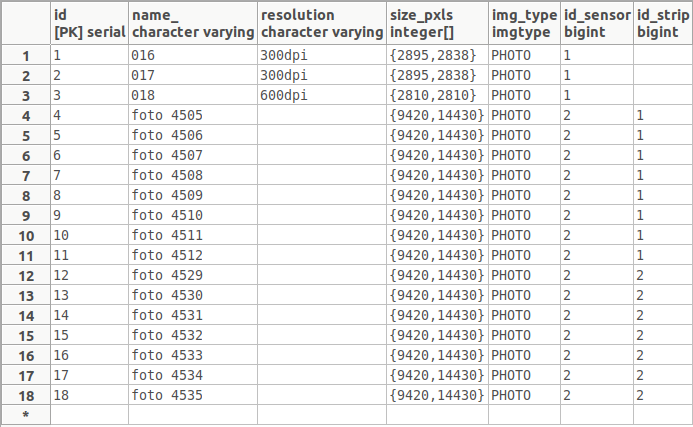
\includegraphics[width=1\hsize]{figuras/img_table.png}
  %\legend{Texto da legenda quando necessário.}
  \source{A autora, 2019.}
\end{figure}

Um banco de dados pode ou não ter a seleção de seus dados armazenados de forma personalizada. Dentre as consultas realizadas, foram elaboradas várias visões. Estas nada mais são que o agrupamento de dados presentes no banco, organizadas de acordo com a programação do usuário. Uma visão pode ser excluída do banco sem que esta signifique que os dados que apresenta sejam perdidos, pois sua exclusão não acarreta na eliminação da tabela original destes dados. Visões também podem ser utilizadas para manter a coerência do banco, auxiliando o DBA a manter um controle do que existe no banco. Um exemplo deste caso é a consulta a seguir:

\begin{lstlisting}
CREATE OR REPLACE VIEW EFOTO.PROJ_LAST_MODIFICATION
AS
SELECT P.NAME_, P.Date_mod
FROM EFOTO.PROJECT P
ORDER BY P.Date_mod DESC;
\end{lstlisting}

A visão deste código apresenta o nome dos projetos existentes no banco, ordenando decrescentemente pela data de modificação. Assim, enquanto não se tem uma forma específica de definir quais projetos estão inativos, esta consulta simples permite ao DBA entender quais projetos não são modificados há mais tempo, o que o auxiliaria na tomada de decisão de manter este projeto no banco ou não. A visão gerada, contendo os dados do banco teste é apresentada na figura \ref{date_mod}.
\begin{figure}[!ht]{10cm}
  \caption{Visão Proj\_last\_modification} \label{date_mod}
  \centering
  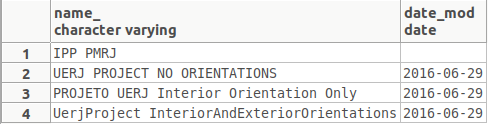
\includegraphics[width=0.8\hsize]{figuras/date_proj.png}
  %\legend{Texto da legenda quando necessário.}
  \source{A autora, 2019.}
\end{figure}
Como visto, nesta visão existe um projeto com o campo de interesse nulo, o que poderia iniciar uma investigação sobre o projeto em questão pelo DBA.

Tratando de consultas à dados fotogramétricos, uma das perguntas feitas foi: \textit{``Quais imagens pertencem à quais projetos?''}, a figura \ref{img_proj}  apresenta 23 tuplas da visão resultante desta pergunta.
\begin{figure}[!ht]{10cm}
  \caption{Visão Img\_proj} \label{img_proj}
  \centering
  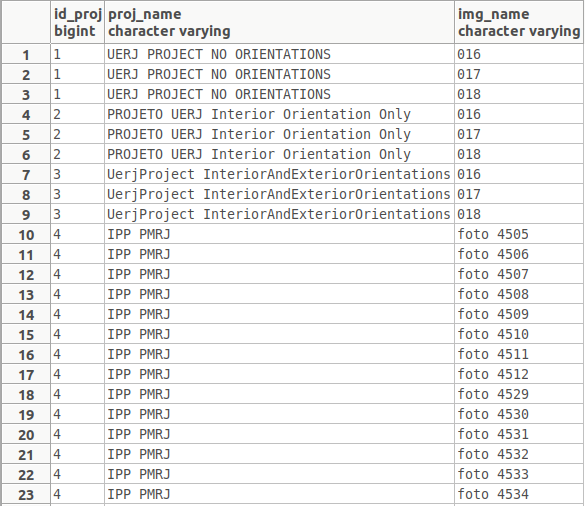
\includegraphics[width=1\hsize]{figuras/img_proj.png}
  %\legend{Texto da legenda quando necessário.}
  \source{A autora, 2019.}
\end{figure}

Como comentado anteriormente ao longo deste trabalho o banco deve ser capaz de armazenar e responder questões sobre dados alfanuméricos e geoespaciais. Assim, perguntas como \textit{``Quais são as coordenadas dos pontos de cada projeto?''}, que pode ser feita também como \textit{``Quais são as coordenadas dos pontos de dado projeto?''} devem ser respondidas. A primeira pode ser respondida numa consulta que, por sua vez, poderia ser uma visão. A segunda pode ser programada como uma função. 

A função \textit{projectpointscoord()}, foi feita para responder justamente esta segunda pergunta. Ao fazer um `select' com esta função, o resultado para o projeto informado pelo usuário, que no caso foi o projeto 4, é apresentado na figura \ref{fun1}. Neste caso o usuário deve somente ter um conhecimento dos índices dos projetos armazenados.

\begin{figure}[!ht]{10cm}
  \caption{Função projectpointscoord} \label{fun1}
  \centering
  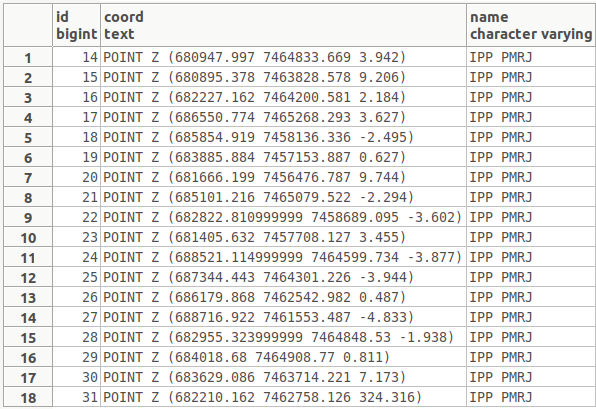
\includegraphics[width=1\hsize]{figuras/fun_ppr.png}
  %\legend{Texto da legenda quando necessário.}
  \source{A autora, 2019.}
\end{figure}

Dessa mesma forma foi criada uma função que responde à consulta: \textit{``Que pontos se encontram dentro de um polígono?''}. Sendo que este polígono poderia ser as delimitações de um ``bounding box'', a projeção de uma foto no terreno ou simplesmente uma área de interesse. O código apresentado a seguir, define a função, \textit{Searchpointsfromgeometry()}, que é capaz de responder esta pergunta.Neste caso os valores de entrada devem estar em WKT, respeitando a sintaxe de um polígono em sql.

\begin{lstlisting}
CREATE OR REPLACE FUNCTION EFOTO.SEARCHPOINTSFROMGEOMETRY(WKT TEXT)
RETURNS TABLE (ID BIGINT, POINT TEXT) AS
$$
SELECT P.ID, ST_AsText(ST_Transform(CAST(P.geom As geometry),32723))
FROM EFOTO.POINT P
WHERE ST_CONTAINS (ST_Transform(ST_GeomFromText(WKT,32723),4326),CAST(P.geom As geometry));
$$ LANGUAGE 'sql';
\end{lstlisting}

Funções, assim como visões, podem ser usadas como ferramentas que testam o banco. Por outro lado ambos os mecanismos podem também facilitar o acesso ao dado pelo usuário comum. A função \textit{Imagekind()} responde ao usuário sobre quais as imagens são de origem digital ou analógica, dependendo somente do usuário informar em qual tipo está interessado. Já a função \textit{EscaleFromImage()} fornece que projetos correspondem ao denominador da escala informada. Neste ponto, para esta última, o usuário deve saber quais valores de escalas estão armazenadas no banco, o que por algumas vezes pode tornar a própria função indesejável, pois antes de executá-la deve ser realizado uma consulta simples que informe quais escalas estão armazenadas no banco de dados. Uma solução para isto é que a função então considere não o denominador de uma escala, mas sim o domínio de denominadores, desde a maior até a menor escala, aumentando, assim, o alcance dessa função.

Com a visão \textit{Image\_file\_found} e sua oposta \textit{Image\_file\_not\_found} é possível saber quais imagens possuem, ou não, arquivos raster armazenados no banco. Isso permite um controle não só do acervo físico do LFSR, mas também auxilia no planejamento das ações tomadas para a aquisição destes arquivos. Estas visões em particular suportam a ideia de que contanto que certos dados dessas imagens sejam conhecidos, como seu local de armazenamento físico, o responsável pelo LFSR será capaz de identificar e realizar um pedido de aquisição para esta foto em caso de imagens de origem analógica, ou arquivo digital em caso de imagens provenientes de imagens digitais.

Um dos questionamentos levantado seria capacidade do banco de responder se: \textit{``O projeto teve sua fase de inicialização finalizada?''}, ou seja, ele está pronto para começar sua geração de produtos? O que de fato define se o projeto já terminou sua fase de inicialização, é a presença dos valores de coeficientes de OI e OE. As visões \textit{Oi\_available} e \textit{Oe\_available} conectam e retornam os valores de cada parâmetro das orientações interior e exterior, às suas respectivas imagens e projetos. As figuras \ref{oi_v} e \ref{oe_v} retornam as visões com os dados até então, carregados no banco de testes.

\begin{figure}[!ht]{13cm}
  \caption{Visão Oi\_available} \label{oi_v}
  \centering
  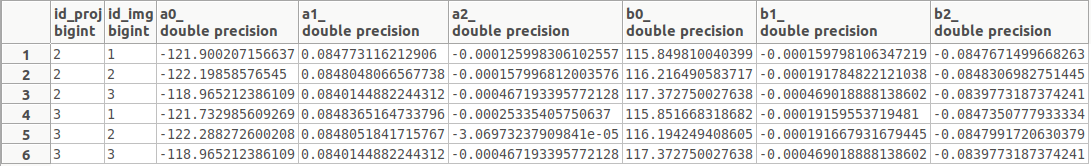
\includegraphics[width=1.1\textwidth, height=0.2\hsize]{figuras/oi.png}
  %\legend{Texto da legenda quando necessário.}
  \source{A autora, 2019.}
\end{figure}
\begin{figure}[!ht]{13cm}
  \caption{Visão Oe\_available} \label{oe_v}
  \centering
  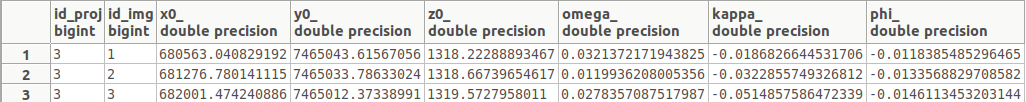
\includegraphics[width=1.1\textwidth, height=0.15\hsize]{figuras/oe.png}
  %\legend{Texto da legenda quando necessário.}
  \source{A autora, 2019.}
\end{figure}

Estas visões por si só, não deixam claro uma resposta para a pergunta em tela. Porém ambas viabilizam a criação de uma nova visão que responda justamente este questionamento. Devido à falta de tempo, a programação e implementação desta visão é prevista em um expansão para o banco de dados. 

Até o momento todas as funções e visões apresentadas foram realizadas separadamente. O código exposto no anexo \ref{script2} comprova que isto não é uma necessidade. Além disto uma pode utilizar da outra para exercer melhor suas finalidades, como é o caso desse código, pois o mesmo expõe os valores dos coeficientes dos parâmetros de OI e OE discutidos acima de uma segunda forma. 

Durante a fase de teste, nem todo o resultado encontrado foi o esperado. Em dado momento, foi levantada a pergunta \textit{``Quantos pontos determinados por Levantamento Topográfico estão armazenados?''}. A resposta dada pelo banco não condizia com a realidade. Neste caso foi investigado qual era a origem deste problema, o que levou à descoberta de um erro no modelo.
Como visto no capítulo \ref{met} existe uma generalização chamada \textit{Survey}, que se especializa nas classes \textit{Ground\_Survey} e \textit{Flight}. Até o momento deste teste, \textit{Collection\_point} realizava uma ligação simples de 1 (um) para 1 (um) com a classe Survey. Isto porém estava errado, pois esta ligação implicava que os pontos de coleções diferentes se confundissem, e o banco, em consequência, duplicava estas coleções sem distinguir de qual levantamento se originavam. A figura \ref{pgs_errado} ilustra a situação ora em questão.

\begin{figure}[!ht]{10cm}
  \caption{Visão Count\_points\_of\_ground\_survey com resultados errados} \label{pgs_errado}
  \centering
  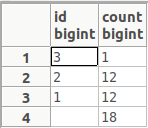
\includegraphics[width=0.3\hsize]{figuras/pgs_errado.png}
  %\legend{Texto da legenda quando necessário.}
  \source{A autora, 2019.}
\end{figure}

Esta ligação então foi refeita ligando as classes \textit{Collection\_point} e \textit{Ground\_Survey}, o que resultou em pequenos ajustes ao longo do modelo. A mesma consulta passou a apresentar os dados de forma correta, como visto na figura \ref{pgs_correto}.

\begin{figure}[!ht]{10cm}
  \caption{Visão Count\_points\_of\_ground\_survey} \label{pgs_correto}
  \centering
  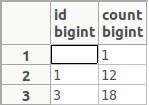
\includegraphics[width=0.3\hsize]{figuras/pgs_correto.png}
  %\legend{Texto da legenda quando necessário.}
  \source{A autora, 2019.}
\end{figure}

Ambas as visões foram geradas graças à consulta abaixo, que define como atributos o índices numéricos de cada \textit{Ground\_Survey} e sua quantidade de pontos, respectivamente.

\begin{lstlisting}

    SELECT GS.ID, COUNT(P.ID)
    FROM EFOTO.POINT P
    LEFT JOIN EFOTO.COLLECTION_POINT CP
    ON P.ID_COLL = CP.ID
    LEFT JOIN EFOTO.GROUND_SURVEY GS
    ON CP.ID_GROUND_SURVEY = GS.ID
    GROUP BY GS.ID ORDER BY COUNT (P.ID);

\end{lstlisting}
Este não foi o único erro descoberto ao longo dos testes, porém todos os problemas encontrados foram resolvidos. Melhorias previstas também foram identificadas, que devido à limitação do tempo, serão deixadas como possíveis expansões para o banco em trabalhos futuros.

Por outro lado, nem todos os contratempos geraram mudanças no modelo. A visualização das imagens armazenadas neste banco de dados piloto não foi feita pelo uso da PgAdmin3. Pois esta interface não têm capacidade de abrir a tabela na qual este arquivo se encontra e nem é idealizada para exibição de imagens. Desta forma foram implementadas duas soluções: a primeira é a presença de um caminho para o local onde o arquivo digital está armazenado, mostrando assim que ele existe no servidor mesmo na hipótese do mesmo não se encontrar fisicamente no banco. A segunda solução foi a visualização dos dados armazenados por meio de outros programas. O script \footnote{Fornecido pelo Professor Irving Badolato, este script é utilizado em suas aulas da disciplina Banco de Dados para ilustrar a recuperação de dados mantidos num servidor PostgreSQl com a extensão Postgis} presente no anexo \ref{script3}, é uma solução que usa o interpretador python para executar um programa descrito desta linguagem e conecta no banco para exibir a imagem armazenada. Para tal, o mesmo faz uso das bibliotecas GDAL, que implementa uma camada de abstração para a manipulação de arquivo de dados geográficos, e o Matplotlib que permite a apresentação de gráficos através de uma janela no Sistema Operacional. Isso prova que podemos expôr o dado em aplicações desenvolvidas no futuro pela equipe do LFSR. Porém, pensando em usuários que não estão familiarizados com a programação, outro meio de visualização dessas imagens foi identificada pela conexão direta com o banco de dados por um software de SIG.

A solução proposta com SIG neste caso é a conexão ao banco pelo QGIS. Neste caso usuário precisa somente se conectar em uma máquina que tenha o acesso ao banco e realizar o acesso pelo software. Feita a conexão o banco as imagens são visualizáveis pelo software QGIS. Nada impede que o usuário procure outros meios de visualização do que os propostos anteriormente. Porém ambos servem para provar que a imagem está acessível pelo banco de dados proposto.

Todos os códigos geradores das funções e visões não referenciados se encontram no apêndice \ref{con}. Ao responder estas e outras perguntas (que tem seus códigos de geração de consulta presentes no apêndice \ref{con}) realizadas pelo responsável de disciplina de fotogrametria do LFSR, o banco pode ser considerado validado.

Devido à complexidade de um processo fotogramétrico e de seus dados, certas limitações se fizeram necessárias para que a realização deste trabalho pudesse cumprir seu prazo estabelecido. Este fato, juntamente com as potencialidades descobertas ao longo do processo, permitiu a previsão de extensões ao modelo elaborado. A modelagem da etapa de produção de um processo fotogramétrico e sua adaptação ao modelo criado por este projeto é um exemplo de expansão prevista. Melhorias que englobem não somente um processo fotogramétrico no nível aéreo, mas também no nível orbital são esperadas e, em alguns casos, sugeridas ao longo do modelo, como discutido neste volume. A criação de uma interface para o banco de dados, vindo a ser este implementado no LFSR, que seja mais amigável ao usuário é também uma possibilidade prevista como extensão e, portanto pode ser desenvolvida em projetos futuros. Por fim, o modelo estabelecido pode ser ampliado para realizar uma integração com a INDE e para possibilitar a execução da restituição estereofotogramétrica diretamente no padrão EDGV. Julga-se que essas atividades sejam passíveis de serem implementadas futuramente no Laboratório.

Vale lembrar que de todos os testes realizados, não houve a realização de nenhum teste de estresse e, que todos os testes e desenvolvimentos explicitados até o presente momento, foram feitos e desenvolvidos para a parte lógica do processo. Desta forma, fica de responsabilidade do LFSR a tomada de decisão de qual espaço físico e como o mesmo será utilizado para a implementação do banco gerado por este trabalho.



\chapter*{Conclusão}
%===================================================================== 
A motivação para a realização deste projeto foi originada a partir da observação das dificuldades de acesso aos dados presentes no acervo do Laboratório de Fotogrametria e Sensoriamento Remoto (LFsR) do Departamento de Engenharia Cartográfica da UERJ, bem como a possibilidade de perda de parte desses dados, devido à sua forma de armazenamento em meio analógico. Assim sendo, foi buscada uma nova forma de armazenar tais dados em caráter permanente provendo uma melhor organização e acesso aos mesmos. O projeto contido neste trabalho apresentou a solução idealizada para o problema exposto. 

Este projeto teve como objetivo a criação de um banco de dados para atender às necessidades do LFSR. A ideia era de que a documentação gerada pudesse replicar o processo de criação desse banco de dados em um servidor de escolha do LFSR, possibilitando o armazenamento do acervo de dados do laboratório. Prevendo o potencial do banco de dados resultante se tornar obsoleto, o mesmo foi modelado para que englobasse também as fases que compunham a etapa de inicialização de um projeto fotogramétrico.

%Como exposto ao longo dos capítulos anteriores, decidiu-se focar no processo fotogramétrico digital que trabalhasse com dados originados da aerofotogrametria tradicional (imagens analógicas digitalizadas). Através da carga de um banco de dados piloto, foi visto que este modelo atende tanto aos dados de origem analógica quanto aos dados digital.

De acordo com os questionamentos e resultados apresentados no capítulo \ref{results} pode-se concluir que o objetivo estabelecido foi alcançado. Este fato pode ser comprovado pela verificação e validação do projeto piloto implementado. Por fim, o item \ref{testefinal} informa a réplica bem sucedida do processo estabelecido neste trabalho por intermédio da documentação gerada pelo mesmo. Logo, conclui-se que o banco, fruto deste processo, é passível de ser implementado em outras máquinas.  

Como sugestões para trabalhos futuros apresentam-se as seguintes:

\begin{itemize}
    \item Melhorias que englobem não somente um processo fotogramétrico no nível aéreo, mas também no nível orbital são esperada;
    \item A criação de uma interface para o banco de dados, que seja mais amigável ao usuário e;
    \item Ampliação do modelo para a integração com a INDE e para possibilitar a execução da restituição estereofotogramétrica diretamente no padrão EDGV.
\end{itemize}



% ----------------------------------------------------------
% ELEMENTOS POS-TEXTUAIS
% ----------------------------------------------------------
\backmatter
%================================================================
% Referencias via BibTeX
%================================================================
\citeoption{abnt-options4}
\bibliography{bibliografia}
%================================================================
% Apêndices e anexos
%================================================================
% %=====================================================================
\postextualchapter*{Glossário}
%=====================================================================
\definicao{termo}{significado}
\definicao{termo}{significado}
 % Caso necessário comente ou descomente as inclusões para os itens postextuais.
% ----------------------------------------------------------
% Apêndices (opcionais)
% ----------------------------------------------------------
% ---
% Inicia os apêndices
% ---
\appendix


%=====================================================================
\postextualchapter{Documentos de casos de uso}\label{ap2}
%=====================================================================
Neste apêndice estão todos os documentos de casos de uso gerado pelo Diagrama de casos de uso.

\begin{table}[!ht]{14cm}
  \caption{Caso de uso Ler Projeto.}
    \begin{tabular}{cc}
    \hline
    \rowcolor[HTML]{333333} 
    {\color[HTML]{FFFFFF} \textbf{Nome do caso de uso}} & {\color[HTML]{FFFFFF} \textbf{Ler Projeto}} \\ \hline
    \rowcolor[HTML]{EFEFEF} 
    \begin{tabular}[c]{@{}c@{}}1.Caso de uso geral\end{tabular} & \begin{tabular}[c]{@{}c@{}} \end{tabular} \\
    \begin{tabular}[c]{@{}c@{}}2.Ator principal \end{tabular} & \begin{tabular}[c]{@{}c@{}} Anônimo\end{tabular} \\
    \rowcolor[HTML]{EFEFEF} 
    \begin{tabular}[c]{@{}c@{}}3.Ator secundário\end{tabular} & \begin{tabular}[c]{@{}c@{}} Aluno, Professor e\\ Administrador\end{tabular} \\
    \begin{tabular}[c]{@{}c@{}}4.Resumo\end{tabular} & \begin{tabular}[c]{@{}c@{}}Este caso de uso consiste na leitura,\\ ou visualização, de um projeto armazenado\\no bando de dados.\end{tabular} \\
    \rowcolor[HTML]{EFEFEF} 
    \begin{tabular}[c]{@{}c@{}}5.Pré-condição\end{tabular} & \begin{tabular}[c]{@{}c@{}}Existir dados públicos \\armazenados no banco de dados\end{tabular} \\
    \begin{tabular}[c]{@{}c@{}}6.Ações do ator\\ I-Acessar banco\\III-Informar login e senha\\ \\ \\VI-Fazer consulta\end{tabular} & \begin{tabular}[c]{@{}c@{}} -Ações do sistema-\\II-Pedir usuário e senha\\IV-Verificar usuário e senha\\V-Permitir acesso de acordo com as restrições \\de tipo de usuário\\ VII- Retornar os dados consultados \end{tabular} \\ 
    \rowcolor[HTML]{EFEFEF} 
    \begin{tabular}[c]{@{}c@{}}7.Restrições e validações
    \end{tabular} & \begin{tabular}[c]{@{}c@{}} O projeto em que contém\\ os dados deve ser público \end{tabular} \\ \hline
    \end{tabular}
  \source{A autora, 2019.}
\end{table}

\begin{table}[!ht]{14cm}
  \caption{Caso de uso Criar Projeto.}
    \begin{tabular}{cc}
    \hline
    \rowcolor[HTML]{333333} 
    {\color[HTML]{FFFFFF} \textbf{Nome do caso de uso}} & {\color[HTML]{FFFFFF} \textbf{Criar Projeto}} \\ \hline
    \rowcolor[HTML]{EFEFEF} 
    \begin{tabular}[c]{@{}c@{}}1.Caso de uso geral\end{tabular} & \begin{tabular}[c]{@{}c@{}} \end{tabular} \\
    \begin{tabular}[c]{@{}c@{}}2.Ator principal \end{tabular} & \begin{tabular}[c]{@{}c@{}}Aluno\end{tabular} \\
    \rowcolor[HTML]{EFEFEF} 
    \begin{tabular}[c]{@{}c@{}}3.Ator secundário\end{tabular} & \begin{tabular}[c]{@{}c@{}}Professor e Administrador\end{tabular} \\
    \begin{tabular}[c]{@{}c@{}}4.Resumo\end{tabular} & \begin{tabular}[c]{@{}c@{}}Este caso de uso consiste na criação\\de um projeto novo dentro do banco de dados \end{tabular} \\
    \rowcolor[HTML]{EFEFEF} 
    \begin{tabular}[c]{@{}c@{}}5.Pré-condição\end{tabular} & \begin{tabular}[c]{@{}c@{}}O login do usuáio ter sido criado\end{tabular} \\
    \begin{tabular}[c]{@{}c@{}}6.Ações do ator\\ I-Acessar banco\\III-Informar login e senha\\ \\ \\VI-Pedir criaação do projeto\end{tabular} & \begin{tabular}[c]{@{}c@{}} -Ações do sistema-\\II-Pedir usuário e senha\\IV-Verificar usuário e senha\\V-Permitir acesso de acordo com as restrições \\de tipo de usuário\\ VII- Criar projeto\end{tabular} \\ 
    \rowcolor[HTML]{EFEFEF} 
    \begin{tabular}[c]{@{}c@{}}7.Restrições e validações
    \end{tabular} & \begin{tabular}[c]{@{}c@{}} O login não ser anônimo \end{tabular} \\ \hline
    \end{tabular}
  \source{A autora, 2019.}
\end{table}

\begin{table}[!ht]{14cm}
  \caption{Caso de uso Editar Projeto.}
    \begin{tabular}{cc}
    \hline
    \rowcolor[HTML]{333333} 
    {\color[HTML]{FFFFFF} \textbf{Nome do caso de uso}} & {\color[HTML]{FFFFFF} \textbf{Editar Projeto}} \\ \hline
    \rowcolor[HTML]{EFEFEF} 
    \begin{tabular}[c]{@{}c@{}}1.Caso de uso geral\end{tabular} & \begin{tabular}[c]{@{}c@{}} \end{tabular} \\
    \begin{tabular}[c]{@{}c@{}}2.Ator principal \end{tabular} & \begin{tabular}[c]{@{}c@{}}Aluno\end{tabular} \\
    \rowcolor[HTML]{EFEFEF} 
    \begin{tabular}[c]{@{}c@{}}3.Ator secundário\end{tabular} & \begin{tabular}[c]{@{}c@{}}Professor e Administrador \end{tabular} \\
    \begin{tabular}[c]{@{}c@{}}4.Resumo\end{tabular} & \begin{tabular}[c]{@{}c@{}} Este caso de uso consiste no\\ armazenamento e edição de dados\\em um banco de dados\end{tabular} \\
    \rowcolor[HTML]{EFEFEF} 
    \begin{tabular}[c]{@{}c@{}}5.Pré-condição\end{tabular} & \begin{tabular}[c]{@{}c@{}}Existir um projeto\end{tabular} \\
    \begin{tabular}[c]{@{}c@{}}6.Ações do ator\\ I-Executar comando de \\armazenamento de dados\\III-Executar comano de edição \\de dados\end{tabular} & \begin{tabular}[c]{@{}c@{}} -Ações do sistema-\\II-Gravar dados\\ \\IV-Editar dados\\ \\V-armazenr alterações nos dados\end{tabular} \\ 
    \rowcolor[HTML]{EFEFEF} 
    \begin{tabular}[c]{@{}c@{}}7.Restrições e validações
    \end{tabular} & \begin{tabular}[c]{@{}c@{}}Projeto deve ser\\ de domínio do usuário\end{tabular} \\ \hline
    \end{tabular}
  \source{A autora, 2019.}
\end{table}

\begin{table}[!ht]{14cm}
  \caption{Caso de uso Deletar Projeto.}
    \begin{tabular}{cc}
    \hline
    \rowcolor[HTML]{333333} 
    {\color[HTML]{FFFFFF} \textbf{Nome do caso de uso}} & {\color[HTML]{FFFFFF} \textbf{Deletar Projeto}} \\ \hline
    \rowcolor[HTML]{EFEFEF} 
    \begin{tabular}[c]{@{}c@{}}1.Caso de uso geral\end{tabular} & \begin{tabular}[c]{@{}c@{}} \end{tabular} \\
    \begin{tabular}[c]{@{}c@{}}2.Ator principal \end{tabular} & \begin{tabular}[c]{@{}c@{}}Aluno\end{tabular} \\
    \rowcolor[HTML]{EFEFEF} 
    \begin{tabular}[c]{@{}c@{}}3.Ator secundário\end{tabular} & \begin{tabular}[c]{@{}c@{}}Professor e Administrador \end{tabular} \\
    \begin{tabular}[c]{@{}c@{}}4.Resumo\end{tabular} & \begin{tabular}[c]{@{}c@{}}Este caso de consiste no ato\\ de deletar um projeto do banco de dados \end{tabular} \\
    \rowcolor[HTML]{EFEFEF} 
    \begin{tabular}[c]{@{}c@{}}5.Pré-condição\end{tabular} & \begin{tabular}[c]{@{}c@{}}Existir um projeto\end{tabular} \\
    \begin{tabular}[c]{@{}c@{}}6.Ações do ator\\ I-Executar comando que delete\\ o projeto\end{tabular} & \begin{tabular}[c]{@{}c@{}} -Ações do sistema-\\II-Deletar projeto\\  \end{tabular} \\ 
    \rowcolor[HTML]{EFEFEF} 
    \begin{tabular}[c]{@{}c@{}}7.Restrições e validações
    \end{tabular} & \begin{tabular}[c]{@{}c@{}}Projeto deve ser de domínio\\do usuário\end{tabular} \\ \hline
    \end{tabular}
  \source{A autora, 2019.}
\end{table}

\begin{table}[!ht]{14cm}
  \caption{Caso de uso Criar Usuário Nível 2.}
    \begin{tabular}{cc}
    \hline
    \rowcolor[HTML]{333333} 
    {\color[HTML]{FFFFFF} \textbf{Nome do caso de uso}} & {\color[HTML]{FFFFFF} \textbf{Criar Usuário Nível 2}} \\ \hline
    \rowcolor[HTML]{EFEFEF} 
    \begin{tabular}[c]{@{}c@{}}1.Caso de uso geral\end{tabular} & \begin{tabular}[c]{@{}c@{}} \end{tabular} \\
    \begin{tabular}[c]{@{}c@{}}2.Ator principal \end{tabular} & \begin{tabular}[c]{@{}c@{}}Professor\end{tabular} \\
    \rowcolor[HTML]{EFEFEF} 
    \begin{tabular}[c]{@{}c@{}}3.Ator secundário\end{tabular} & \begin{tabular}[c]{@{}c@{}}Aluno\end{tabular} \\
    \begin{tabular}[c]{@{}c@{}}4.Resumo\end{tabular} & \begin{tabular}[c]{@{}c@{}}Este caso de uso consiste na\\ criação de um usuário do nível 2\end{tabular} \\
    \rowcolor[HTML]{EFEFEF} 
    \begin{tabular}[c]{@{}c@{}}5.Pré-condição\end{tabular} & \begin{tabular}[c]{@{}c@{}}Login do usuário ser\\ Professor ou Administrador\end{tabular} \\
    \begin{tabular}[c]{@{}c@{}}6.Ações do ator\\ I-Preencher dados de novo usuário\\II-Mandar criar novo usuário\\ \\ \\ \\\end{tabular} & \begin{tabular}[c]{@{}c@{}} -Ações do sistema-\\ \\III-Checar se o usuário tem permissão \\ para criai o usuário nível 2\\IV-Criar usuário\end{tabular} \\ 
    \rowcolor[HTML]{EFEFEF} 
    \begin{tabular}[c]{@{}c@{}}7.Restrições e validações
    \end{tabular} & \begin{tabular}[c]{@{}c@{}}O usuário a ser criado\\ deve se de nível 2\end{tabular} \\ \hline
    \end{tabular}
  \source{A autora, 2019.}
\end{table}

\begin{table}[!ht]{14cm}
  \caption{Caso de uso Editar Usuário de Nível 2.}
    \begin{tabular}{cc}
    \hline
    \rowcolor[HTML]{333333} 
    {\color[HTML]{FFFFFF} \textbf{Nome do caso de uso}} & {\color[HTML]{FFFFFF} \textbf{Editar Usuário de Nível 2}} \\ \hline
    \rowcolor[HTML]{EFEFEF} 
    \begin{tabular}[c]{@{}c@{}}1.Caso de uso geral\end{tabular} & \begin{tabular}[c]{@{}c@{}} \end{tabular} \\
    \begin{tabular}[c]{@{}c@{}}2.Ator principal \end{tabular} & \begin{tabular}[c]{@{}c@{}}Professor\end{tabular} \\
    \rowcolor[HTML]{EFEFEF} 
    \begin{tabular}[c]{@{}c@{}}3.Ator secundário\end{tabular} & \begin{tabular}[c]{@{}c@{}}Administrador\end{tabular} \\
    \begin{tabular}[c]{@{}c@{}}4.Resumo\end{tabular} & \begin{tabular}[c]{@{}c@{}}Este caso consiste em  editar os dados\\ de um usuário nível 2\end{tabular} \\
    \rowcolor[HTML]{EFEFEF} 
    \begin{tabular}[c]{@{}c@{}}5.Pré-condição\end{tabular} & \begin{tabular}[c]{@{}c@{}}Existir o usuário\end{tabular} \\
    \begin{tabular}[c]{@{}c@{}}6.Ações do ator\\ I-Pedir acesso ao dados\\do usuário\\IV-Acessar usuário\\ \\V-Alterar dados do usuário \\ \end{tabular} & \begin{tabular}[c]{@{}c@{}} -Ações do sistema-\\II-Verificar permissão de acesso\\do usuário professor\\III-Disponibilizar dados ao usuário \\professor\\VI-Armazenar alterações de dados\\ do usuário \end{tabular} \\ 
    \rowcolor[HTML]{EFEFEF} 
    \begin{tabular}[c]{@{}c@{}}7.Restrições e validações
    \end{tabular} & \begin{tabular}[c]{@{}c@{}}Usuário a ser editado ser\\do nível 2\\Usuário a ser editado se do domínio \\do usuário professor  \end{tabular} \\ \hline
    \end{tabular}
  \source{A autora, 2019.}
\end{table}

\begin{table}[!ht]{14cm}
  \caption{Caso de uso Deletar Usuário nível 2.}
    \begin{tabular}{cc}
    \hline
    \rowcolor[HTML]{333333} 
    {\color[HTML]{FFFFFF} \textbf{Nome do caso de uso}} & {\color[HTML]{FFFFFF} \textbf{Deletar Usuário Nível 2}} \\ \hline
    \rowcolor[HTML]{EFEFEF} 
    \begin{tabular}[c]{@{}c@{}}1.Caso de uso geral\end{tabular} & \begin{tabular}[c]{@{}c@{}} \end{tabular} \\
    \begin{tabular}[c]{@{}c@{}}2.Ator principal \end{tabular} & \begin{tabular}[c]{@{}c@{}}Professor\end{tabular} \\
    \rowcolor[HTML]{EFEFEF} 
    \begin{tabular}[c]{@{}c@{}}3.Ator secundário\end{tabular} & \begin{tabular}[c]{@{}c@{}}Aluno \end{tabular} \\
    \begin{tabular}[c]{@{}c@{}}4.Resumo\end{tabular} & \begin{tabular}[c]{@{}c@{}}Este caso de uso consiste em deletar um \\ usuário nível 2\end{tabular} \\
    \rowcolor[HTML]{EFEFEF} 
    \begin{tabular}[c]{@{}c@{}}5.Pré-condição\end{tabular} & \begin{tabular}[c]{@{}c@{}}Existiŕ o usuário\end{tabular} \\
    \begin{tabular}[c]{@{}c@{}}6.Ações do ator\\ I-Comandar deletar usuário\\III-Confirmar\end{tabular} & \begin{tabular}[c]{@{}c@{}} -Ações do sistema-\\II-Verificar permissão do usuário \\IV-Deletar usuário\end{tabular} \\ 
    \rowcolor[HTML]{EFEFEF} 
    \begin{tabular}[c]{@{}c@{}}7.Restrições e validações
    \end{tabular} & \begin{tabular}[c]{@{}c@{}} Usuário deletado ser de nível 2\\Usuário deletado ser de domínio \\ do usuário professor\end{tabular} \\ \hline
    \end{tabular}
  \source{A autora, 2019.}
\end{table}

\begin{table}[!ht]{14cm}
  \caption{Caso de uso Criar Usuário.}
    \begin{tabular}{cc}
    \hline
    \rowcolor[HTML]{333333} 
    {\color[HTML]{FFFFFF} \textbf{Nome do caso de uso}} & {\color[HTML]{FFFFFF} \textbf{Criar Usuário}} \\ \hline
    \rowcolor[HTML]{EFEFEF} 
    \begin{tabular}[c]{@{}c@{}}1.Caso de uso geral\end{tabular} & \begin{tabular}[c]{@{}c@{}} \end{tabular} \\
    \begin{tabular}[c]{@{}c@{}}2.Ator principal \end{tabular} & \begin{tabular}[c]{@{}c@{}}Administrador\end{tabular} \\
    \rowcolor[HTML]{EFEFEF} 
    \begin{tabular}[c]{@{}c@{}}3.Ator secundário\end{tabular} & \begin{tabular}[c]{@{}c@{}}\end{tabular} \\
    \begin{tabular}[c]{@{}c@{}}4.Resumo\end{tabular} & \begin{tabular}[c]{@{}c@{}}Este caso de uso de consiste na \\criação de um usuário dentro do banco\\ de dados\end{tabular} \\
    \rowcolor[HTML]{EFEFEF} 
    \begin{tabular}[c]{@{}c@{}}5.Pré-condição\end{tabular} & \begin{tabular}[c]{@{}c@{}}\end{tabular} \\
    \begin{tabular}[c]{@{}c@{}}6.Ações do ator\\ I-Preencher dados de um novo usuário\\II-Definir restrições do usuário\\III-Mandar criar novo usuário\\ \\ \\ \end{tabular} & \begin{tabular}[c]{@{}c@{}} -Ações do sistema-\\ \\ \\ \\IV-Checar se o usuário tem permissão\\ para criar usuário\\V-Criar usuário \end{tabular} \\ 
    \rowcolor[HTML]{EFEFEF} 
    \begin{tabular}[c]{@{}c@{}}7.Restrições e validações
    \end{tabular} & \begin{tabular}[c]{@{}c@{}} \end{tabular} \\ \hline
    \end{tabular}
  \source{A autora, 2019.}
\end{table}

\begin{table}[!ht]{14cm}
  \caption{Caso de uso Editar Usuário.}
    \begin{tabular}{cc}
    \hline
    \rowcolor[HTML]{333333} 
    {\color[HTML]{FFFFFF} \textbf{Nome do caso de uso}} & {\color[HTML]{FFFFFF} \textbf{Editar usuário}} \\ \hline
    \rowcolor[HTML]{EFEFEF} 
    \begin{tabular}[c]{@{}c@{}}1.Caso de uso geral\end{tabular} & \begin{tabular}[c]{@{}c@{}} \end{tabular} \\
    \begin{tabular}[c]{@{}c@{}}2.Ator principal \end{tabular} & \begin{tabular}[c]{@{}c@{}}Administrador\end{tabular} \\
    \rowcolor[HTML]{EFEFEF} 
    \begin{tabular}[c]{@{}c@{}}3.Ator secundário\end{tabular} & \begin{tabular}[c]{@{}c@{}} \end{tabular} \\
    \begin{tabular}[c]{@{}c@{}}4.Resumo\end{tabular} & \begin{tabular}[c]{@{}c@{}}Este caso de uso consiste na edição de \\ um usuário do banco de dados \end{tabular} \\
    \rowcolor[HTML]{EFEFEF} 
    \begin{tabular}[c]{@{}c@{}}5.Pré-condição\end{tabular} & \begin{tabular}[c]{@{}c@{}}Existir usuário a ser modificado\end{tabular} \\
    \begin{tabular}[c]{@{}c@{}}6.Ações do ator\\ I-Pedir acesso ao dados\\do usuário\\IV-Acessar usuário\\ \\V-Alterar dados do usuário \\ \\ \end{tabular} & \begin{tabular}[c]{@{}c@{}} -Ações do sistema-\\II-Verificar permissão de acesso\\do usuário professor\\III-Disponibilizar dados ao usuário \\professor\\VI-Armazenar alterações de dados\\ do usuário \end{tabular} \\ 
    \rowcolor[HTML]{EFEFEF} 
    \begin{tabular}[c]{@{}c@{}}7.Restrições e validações
    \end{tabular} & \begin{tabular}[c]{@{}c@{}} \end{tabular} \\ \hline
    \end{tabular}
  \source{A autora, 2019.}
\end{table}

\begin{table}[!ht]{14cm}
  \caption{Caso de uso Deletar Usuário.}
    \begin{tabular}{cc}
    \hline
    \rowcolor[HTML]{333333} 
    {\color[HTML]{FFFFFF} \textbf{Nome do caso de uso}} & {\color[HTML]{FFFFFF} \textbf{Deletar Usuário}} \\ \hline
    \rowcolor[HTML]{EFEFEF} 
    \begin{tabular}[c]{@{}c@{}}1.Caso de uso geral\end{tabular} & \begin{tabular}[c]{@{}c@{}} \end{tabular} \\
    \begin{tabular}[c]{@{}c@{}}2.Ator principal \end{tabular} & \begin{tabular}[c]{@{}c@{}}Administrador\end{tabular} \\
    \rowcolor[HTML]{EFEFEF} 
    \begin{tabular}[c]{@{}c@{}}3.Ator secundário\end{tabular} & \begin{tabular}[c]{@{}c@{}} \end{tabular} \\
    \begin{tabular}[c]{@{}c@{}}4.Resumo\end{tabular} & \begin{tabular}[c]{@{}c@{}}Este caso de uso consiste na ação de deletar\\ um usuário do banco de dados \end{tabular} \\
    \rowcolor[HTML]{EFEFEF} 
    \begin{tabular}[c]{@{}c@{}}5.Pré-condição\end{tabular} & \begin{tabular}[c]{@{}c@{}}\end{tabular} \\
    \begin{tabular}[c]{@{}c@{}}6.Ações do ator\\ I-Mandar deletar o usuário\\ \\IV-Confirmar\end{tabular} & \begin{tabular}[c]{@{}c@{}} -Ações do sistema-\\II-Verificar permissão\\III-Enviar mensagem pedindo confirmação\\V-Deletar usuário\end{tabular} \\ 
    \rowcolor[HTML]{EFEFEF} 
    \begin{tabular}[c]{@{}c@{}}7.Restrições e validações
    \end{tabular} & \begin{tabular}[c]{@{}c@{}} \end{tabular} \\ \hline
    \end{tabular}
  \source{A autora, 2019.}
\end{table}




%=====================================================================
\postextualchapter{Modelo do banco de dados}
%=====================================================================

\section{Especificação de Classes}\label{ap0}

\begin{figure}[!ht]{10cm}
  \caption{Classe Project} \label{project}
  \centering
  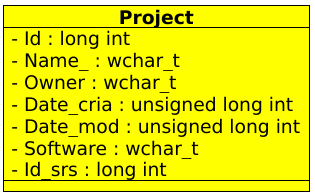
\includegraphics[width=0.5\hsize]{figuras/31.png}
  %\legend{Texto da legenda quando necessário.}
  \source{A autora, 2019.}
\end{figure}

\begin{figure}[!ht]{5cm}
  \caption{Classe Srs} \label{srs}
  \centering
  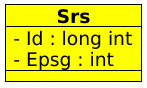
\includegraphics[width=0.5\hsize]{figuras/33.png}
  %\legend{Texto da legenda quando necessário.}
  \source{A autora, 2019.}
\end{figure}

\begin{figure}[!ht]{6cm}
  \caption{Classe Cg\_central\_area} \label{cg}
  \centering
  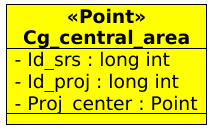
\includegraphics[width=0.6\hsize]{figuras/32.png}
  %\legend{Texto da legenda quando necessário.}
  \source{A autora, 2019.}
\end{figure}

\begin{figure}[!ht]{6cm}
  \caption{Classe Terrain} \label{terrain}
  \centering
  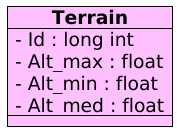
\includegraphics[width=0.6\hsize]{figuras/37.png}
  %\legend{Texto da legenda quando necessário.}
  \source{A autora, 2019.}
\end{figure}

\begin{figure}[!ht]{10cm}
  \caption{Classe Flight} \label{flight}
  \centering
  \includegraphics[width=0.6\hsize]{figuras/34.png}
  %\legend{Texto da legenda quando necessário.}
  \source{A autora, 2019.}
\end{figure}

\begin{figure}[!ht]{10cm}
  \caption{Classe Param\_flight} \label{parm_flight}
  \centering
  \includegraphics[width=0.5\hsize]{figuras/35.png}
  %\legend{Texto da legenda quando necessário.}
  \source{A autora, 2019.}
\end{figure}

\begin{figure}[!ht]{6cm}
  \caption{Classe Bouding\_box} \label{bbox}
  \centering
  \includegraphics[width=0.7\hsize]{figuras/36.png}
  %\legend{Texto da legenda quando necessário.}
  \source{A autora, 2019.}
\end{figure}

\begin{figure}[!ht]{6cm}
  \caption{Classe Sensor} \label{sensor}
  \centering
  \includegraphics[width=0.8\hsize]{figuras/41.png}
  %\legend{Texto da legenda quando necessário.}
  \source{A autora, 2019.}
\end{figure}

\begin{figure}[!ht]{10cm}
  \caption{Classe Specification} \label{spec}
  \centering
  \includegraphics[width=0.5\hsize]{figuras/42.png}
  %\legend{Texto da legenda quando necessário.}
  \source{A autora, 2019.}
\end{figure}

\begin{figure}[!ht]{10cm}
  \caption{Data type Sensor\_type } \label{typesensor}
  \centering
  \includegraphics[width=0.4\hsize]{figuras/45.png}
  %\legend{Texto da legenda quando necessário.}
  \source{A autora, 2019.}
\end{figure}

\begin{figure}[!ht]{10cm}
  \caption{Classe Calibration} \label{calib}
  \centering
  \includegraphics[width=0.6\hsize]{figuras/39.png}
  %\legend{Texto da legenda quando necessário.}
  \source{A autora, 2019.}
\end{figure}

\begin{figure}[!ht]{6cm}
  \caption{Classe Fiducials} \label{fid}
  \centering
  \includegraphics[width=0.75\hsize]{figuras/38.png}
  %\legend{Texto da legenda quando necessário.}
  \source{A autora, 2019.}
\end{figure}

\begin{figure}[!ht]{10cm}
  \caption{Classe Symmetric\_distortion} \label{sym}
  \centering
  \includegraphics[width=0.5\hsize]{figuras/43.png}
  %\legend{Texto da legenda quando necessário.}
  \source{A autora, 2019.}
\end{figure}

\begin{figure}[!ht]{6cm}
  \caption{Classe Decentering\_distortion} \label{dis}
  \centering
  \includegraphics[width=0.75\hsize]{figuras/40.png}
  %\legend{Texto da legenda quando necessário.}
  \source{A autora, 2019.}
\end{figure}

\begin{figure}[!ht]{6cm}
  \caption{Classe Point} \label{point}
  \centering
  \includegraphics[width=1\hsize]{figuras/30.png}
  %\legend{Texto da legenda quando necessário.}
  \source{A autora, 2019.}
\end{figure}

\begin{figure}[!ht]{10cm}
  \caption{Classe Collection\_Point} \label{collpoint}
  \centering
  \includegraphics[width=0.6\hsize]{figuras/29.png}
  %\legend{Texto da legenda quando necessário.}
  \source{A autora, 2019.}
\end{figure}

\begin{figure}[!ht]{6cm}
  \caption{Classe Point\_project} \label{pointpro}
  \centering
  \includegraphics[width=0.8\hsize]{figuras/22.png}
  %\legend{Texto da legenda quando necessário.}
  \source{A autora, 2019.}
\end{figure}

\begin{figure}[!ht]{6cm}
  \caption{Data type Pointtype} \label{pointype}
  \centering
  \includegraphics[width=0.8\hsize]{figuras/24.png}
  %\legend{Texto da legenda quando necessário.}
  \source{A autora, 2019.}
\end{figure}

\begin{figure}[!ht]{6cm}
  \caption{Classe Ground\_survey} \label{gp}
  \centering
  \includegraphics[width=0.8\hsize]{figuras/27.png}
  %\legend{Texto da legenda quando necessário.}
  \source{A autora, 2019}
\end{figure}

\begin{figure}[!ht]{6cm}
  \caption{Classe Measure} \label{meas}
  \centering
  \includegraphics[width=0.6\hsize]{figuras/21.png}
  %\legend{Texto da legenda quando necessário.}
  \source{A autora, 2019}
\end{figure}

\begin{figure}[!ht]{10cm}
  \caption{Classe Image} \label{img}
  \centering
  \includegraphics[width=0.5\hsize]{figuras/6.png}
  %\legend{Texto da legenda quando necessário.}
  \source{A autora, 2019}
\end{figure}

\begin{figure}[!ht]{6cm}
  \caption{Data type Imgtype} \label{imgt}
  \centering
  \includegraphics[width=0.8\hsize]{figuras/25.png}
  %\legend{Texto da legenda quando necessário.}
  \source{A autora, 2019}
\end{figure}

\begin{figure}[!ht]{6cm}
  \caption{Classe File\_img} \label{file}
  \centering
  \includegraphics[width=0.75\hsize]{figuras/19.png}
  %\legend{Texto da legenda quando necessário.}
  \source{A autora, 2019}
\end{figure}

\begin{figure}[!ht]{6cm}
  \caption{Classe Tn} \label{tn}
  \centering
  \includegraphics[width=0.55\hsize]{figuras/18.png}
  %\legend{Texto da legenda quando necessário.}
  \source{A autora, 2019}
\end{figure}

\begin{figure}[!ht]{6cm}
  \caption{Classe Photo} \label{photo}
  \centering
  \includegraphics[width=0.8\hsize]{figuras/3.png}
  %\legend{Texto da legenda quando necessário.}
  \source{A autora, 2019}
\end{figure}

\begin{figure}[!ht]{6cm}
  \caption{Data type Typephoto} \label{tp}
  \centering
  \includegraphics[width=0.8\hsize]{figuras/26.png}
  %\legend{Texto da legenda quando necessário.}
  \source{A autora, 2019}
\end{figure}

\begin{figure}[!ht]{6cm}
  \caption{Classe Frame} \label{fram}
  \centering
  \includegraphics[width=0.75\hsize]{figuras/2.png}
  %\legend{Texto da legenda quando necessário.}
  \source{A autora, 2019}
\end{figure}

\begin{figure}[!ht]{6cm}
  \caption{Classe Strip} \label{strip}
  \centering
  \includegraphics[width=0.7\hsize]{figuras/16.png}
  %\legend{Texto da legenda quando necessário.}
  \source{A autora, 2019}
\end{figure}

\begin{figure}[!ht]{6cm}
  \caption{Classe Block} \label{blo}
  \centering
  \includegraphics[width=0.65\hsize]{figuras/17.png}
  %\legend{Texto da legenda quando necessário.}
  \source{A autora, 2019}
\end{figure}

\begin{figure}[!ht]{6cm}
  \caption{Classe Img\_block} \label{imgblo}
  \centering
  \includegraphics[width=0.7\hsize]{figuras/20.png}
  %\legend{Texto da legenda quando necessário.}
  \source{A autora, 2019}
\end{figure}

\begin{figure}[!ht]{6cm}
  \caption{Classe Pair} \label{pair}
  \centering
  \includegraphics[width=0.75\hsize]{figuras/8.png}
  %\legend{Texto da legenda quando necessário.}
  \source{A autora, 2019}
\end{figure}

\begin{figure}[!ht]{6cm}
  \caption{Classe Coverage} \label{comm}
  \centering
  \includegraphics[width=0.75\hsize]{figuras/5.png}
  %\legend{Texto da legenda quando necessário.}
  \source{A autora, 2019}
\end{figure}

\begin{figure}[!ht]{6cm}
  \caption{Classe Common\_coverage} \label{comcov}
  \centering
  \includegraphics[width=0.85\hsize]{figuras/9.png}
  %\legend{Texto da legenda quando necessário.}
  \source{A autora, 2019}
\end{figure}

\begin{figure}[!ht]{6cm}
  \caption{Classe Ntuplet} \label{ntu}
  \centering
  \includegraphics[width=0.7\hsize]{figuras/12.png}
  %\legend{Texto da legenda quando necessário.}
  \source{A autora, 2019}
\end{figure}

\begin{figure}[!ht]{6cm}
  \caption{Classe Img\_ntuplet} \label{imgtu}
  \centering
  \includegraphics[width=0.7\hsize]{figuras/14.png}
  %\legend{Texto da legenda quando necessário.}
  \source{A autora, 2019}
\end{figure}

\begin{figure}[!ht]{6cm}
  \caption{Classe Mod\_param} \label{modpar}
  \centering
  \includegraphics[width=0.7\hsize]{figuras/11.png}
  %\legend{Texto da legenda quando necessário.}
  \source{A autora, 2019}
\end{figure}

\begin{figure}[!ht]{6cm}
  \caption{Data type Type\_op} \label{top}
  \centering
  \includegraphics[width=0.6\hsize]{figuras/23.png}
  %\legend{Texto da legenda quando necessário.}
  \source{A autora, 2019}
\end{figure}

\begin{figure}[!ht]{6cm}
  \caption{Classe Parameter} \label{par}
  \centering
  \includegraphics[width=0.7\hsize]{figuras/7.png}
  %\legend{Texto da legenda quando necessário.}
  \source{A autora, 2019}
\end{figure}

\begin{figure}[!ht]{6cm}
  \caption{Classe Coef\_img} \label{coefimg}
  \centering
  \includegraphics[width=0.8\hsize]{figuras/15.png}
  %\legend{Texto da legenda quando necessário.}
  \source{A autora, 2019}
\end{figure}

\begin{figure}[!ht]{10cm}
  \caption{Classe Processing\_metho} \label{proces}
  \centering
  \includegraphics[width=0.5\hsize]{figuras/44.png}
  %\legend{Texto da legenda quando necessário.}
  \source{A autora, 2019}
\end{figure}

\begin{figure}[!ht]{6cm}
  \caption{Classe Frame\_gnss} \label{gnss}
  \centering
  \includegraphics[width=1\hsize]{figuras/1.png}
  %\legend{Texto da legenda quando necessário.}
  \source{A autora, 2019}
\end{figure}

\begin{figure}[!ht]{6cm}
  \caption{Classe Frame\_ins} \label{ins}
  \centering
  \includegraphics[width=0.65\hsize]{figuras/4.png}
  %\legend{Texto da legenda quando necessário.}
  \source{A autora, 2019}
\end{figure}


\section{Modelos completos}\label{ap-1}
\begin{landscape}
\begin{figure}[ht]{21cm}
  \caption{Modelo Orientado à Objeto.} \label{modelo_00}
  \includegraphics[width=\hsize]{figuras/modelo_oo.png}
  \legend{Imagem gerada com o software Umbrello.}
  \source{A autora, 2019}
\end{figure}
\end{landscape}

\begin{landscape}
\begin{figure}[ht]{25cm}
  \caption{Modelo Relacional.} \label{modelo_r}
  \includegraphics[width=\hsize]{figuras/modelo_er.png}
  \legend{Imagem gerada com a plataforma online ERDPlus.}
  \source{A autora, 2019}
\end{figure}
\end{landscape}





%=====================================================================
\postextualchapter{Códigos}\label{ap1}
%=====================================================================
\section{Código para o Banco de Dados}\label{cdg}

Código para a criação do Projeto Piloto do Banco de Dados.
\lstinputlisting[]{codigos/cdgbanco.sql}

\section{Cargas}\label{crg}
Código de cargas realizadas no banco
\subsection{Primeira Carga} \label{carga1}
\lstinputlisting[]{codigos/carga1.sql}
\subsection{Segunda Carga}\label{carga2}
\lstinputlisting[]{codigos/carga2.sql}
\subsection{Terceira Carga}\label{carga3}
\lstinputlisting[]{codigos/carga_img.sh}

\section{Consultas}\label{con}
Código das funções e visões usadas para testar o Banco de Dados
\subsection{Visões}\label{visoes}
\lstinputlisting[]{codigos/quest_views.sql}
\subsection{Funções}\label{funcoes}
\lstinputlisting[]{codigos/quest_functions.sql}


% ----------------------------------------------------------
% Anexos (opcionais)
% ----------------------------------------------------------
% ---
% Inicia os anexos
% ---
\annex
%=====================================================================
\postextualchapter{\textit{Scripts} em Python para o carregamento e visualização de imagens}
%=====================================================================

Códigos complementares para operacionalização imediata no Banco de Dados que foram cedidos pelo Prof. Irving Badolato ao longo da execução deste trabalho.

\section{Carregamento de imagens}\label{script1}
\lstinputlisting[language=python,showstringspaces=false]{codigos/storeimgs.py}

\section{Exemplo de para a visualização de imagens carregadas no SGBD}\label{script3}
\lstinputlisting[language=python,showstringspaces=false]{codigos/rastertest.py}

O exemplo apresentado nesta seção depende de um módulo de nome dbconn, cujo código implementa uma interface gráfica com o usuário. A implementação de dbconn, no arquivo \textit{dbconn.py}, contém:

\lstinputlisting[language=python,showstringspaces=false]{codigos/dbconn.py}


%=====================================================================
\postextualchapter{Consulta dos parâmetros de orientação das imagens}
%=====================================================================

\section{Exemplo de função e visão como alternativa de recuperar os parâmetros de Orientação Interior}\label{script2}
\lstinputlisting[]{codigos/ios.sql}

%---------------------------------------------------------------------
% INDICE REMISSIVO (relativo ao makeindex)
%---------------------------------------------------------------------
\printindex

%=====================================================================
\end{document}
